\chapter{Topology and Linear Algebra}
\label{ch:topology-linear-algebra}

In one variable, $|x-y|$ measures distance, one number $f'(a)$ describes
the best linear approximation, and substitution rescales a short interval.
In several variables these three familiar operations separate into several
ideas. A point is now a vector, and proximity must make sense without
privileging one coordinate. A derivative sends an input displacement to an
output displacement: it is a linear transformation. Its Jacobian matrix is
the table representing that transformation in chosen coordinates, not the
transformation itself. Substitution must measure the volume distortion of a
small box; the absolute determinant gives its magnitude, while the sign
records orientation. Finally, forms evaluate several tangent directions at
once, requiring dual spaces and alternating multilinear maps.

This chapter is not trying to reproduce full courses in topology and linear
algebra. It develops the parts of those subjects needed for Chapters 11--13,
but develops those parts carefully enough that they do not become hidden
prerequisites. Our roadmap is
\[
\begin{gathered}
\text{distance and neighborhoods}\longrightarrow\text{compactness and continuity}\\
\longrightarrow\text{vectors and linear maps}\longrightarrow\text{matrices and coordinates}\\
\longrightarrow\text{inner products and norms}\longrightarrow\text{multilinearity}\\
\longrightarrow\text{determinants and orientation}.
\end{gathered}
\]
Keep asking two questions: what is the object, and which numbers describe
it? A coordinate column, a matrix, and a covector row will answer different
questions even when all three are arrays of real numbers.

\section{Distances, Balls, and Neighborhoods}
On $\R$, distance is $|x-y|$. In the plane the Pythagorean theorem gives
\[
d_2(x,y)=\sqrt{(x_1-y_1)^2+(x_2-y_2)^2}.
\]
In $\R^n$ define the \emph{Euclidean length}
\[
\|x\|_2=\left(\sum_{j=1}^n x_j^2\right)^{1/2},
\qquad d_2(x,y)=\|x-y\|_2.
\]
We call this a length for the moment: the triangle inequality, and hence
the fact that it is a norm, will follow from Cauchy--Schwarz below.
Which properties of distance actually enter convergence and continuity
arguments? Zero distance identifies a point, reversing the two points changes
nothing, and an intermediate stop cannot shorten the trip. We abstract these
properties, then verify that the Euclidean formula has them.
\begin{definition}[Metric space]
A metric on $X$ is a map $d:X\times X\to[0,\infty)$ satisfying, for all
$x,y,z\in X$,
\begin{align*}
d(x,y)=0&\ \Longleftrightarrow\ x=y &&\text{(identity of indiscernibles)},\\
d(x,y)&=d(y,x) &&\text{(symmetry)},\\
d(x,z)&\leq d(x,y)+d(y,z) &&\text{(triangle inequality)}.
\end{align*}
The pair $(X,d)$ is a metric space.
\end{definition}
\begin{theorem}[Cauchy--Schwarz inequality]\label{thm:cauchy-schwarz}
Writing $x\cdot y=\sum_jx_jy_j$ and $\|x\|_2=\sqrt{x\cdot x}$, we have
$|x\cdot y|\leq\|x\|_2\|y\|_2$. Consequently $\|\cdot\|_2$ is a norm
and $d_2(x,y)=\|x-y\|_2$ is its associated metric.
\end{theorem}
\begin{proof}
The triangle inequality for Euclidean length contains the cross term
$2u\cdot v$. We therefore establish Cauchy--Schwarz first; it is exactly
the estimate that controls this term.
If $y=0$ the inequality reads $0\leq0$. Otherwise substitute
$t=(x\cdot y)/\|y\|_2^2$ into a sum of squares. This value is chosen
because
\[
\norm{x-ty}_2^2
=\norm x_2^2-2t(x\cdot y)+t^2\norm y_2^2
\]
is a nonnegative quadratic in $t$, minimized when
$t=(x\cdot y)/\norm y_2^2$ (equivalently, this choice completes the
square). At its minimum,
\[
0\leq\sum_j(x_j-ty_j)^2
=\|x\|_2^2-\frac{(x\cdot y)^2}{\|y\|_2^2}.
\]
Multiplication by $\|y\|_2^2$ and square roots give the assertion. For
$u=x-y$ and $v=y-z$, it follows that
\[
\|u+v\|_2^2=\|u\|_2^2+2u\cdot v+\|v\|_2^2
\leq(\|u\|_2+\|v\|_2)^2.
\]
Taking square roots proves the triangle inequality. A sum of nonnegative
squares is zero exactly when every coordinate is zero, and
$\|\alpha x\|_2=|\alpha|\|x\|_2$. Thus Euclidean length satisfies all
three norm axioms. Applying definiteness to $x-y$ and observing that
$\|x-y\|_2=\|y-x\|_2$ verify the remaining metric axioms for $d_2$.
\end{proof}

From now on, unless another norm is explicitly indicated, the standing
convention on Euclidean space is
\[
\boxed{\|x\|:=\|x\|_2\qquad(x\in\R^n).}
\]
The later abstract treatment of norms generalizes this notation; it does
not change the present Euclidean convention.

The points within distance $r>0$ of $a$ form $(a-r,a+r)$ on the line
and an open disk in the plane. The limiting endpoints or circle are excluded.
\begin{center}
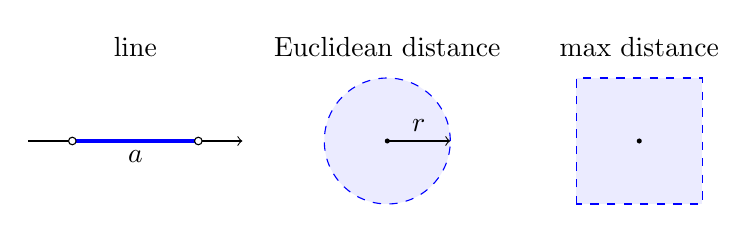
\begin{tikzpicture}[scale=.8]
\draw[->] (-1.7,0)--(1.7,0); \draw[very thick,blue] (-1,0)--(1,0);
\draw[fill=white] (-1,0) circle (.06) (1,0) circle (.06);
\node[below] at (0,0) {$a$}; \node at (0,1.5) {line};
\begin{scope}[xshift=4cm]
\fill[blue!8] (0,0) circle (1); \draw[dashed,blue] (0,0) circle (1);
\fill (0,0) circle (.04); \draw[->] (0,0)--(1,0) node[midway,above] {$r$};
\node at (0,1.5) {Euclidean distance};
\end{scope}
\begin{scope}[xshift=8cm]
\fill[blue!8] (-1,-1) rectangle (1,1);
\draw[dashed,blue] (-1,-1) rectangle (1,1);
\fill (0,0) circle (.04); \node at (0,1.5) {max distance};
\end{scope}
\end{tikzpicture}
\end{center}
\begin{definition}[Balls and neighborhoods]
The open ball of center $a$ and radius $r>0$ is
\[
B_d(a,r)=\{x\in X:d(x,a)<r\}.
\]
A \textbf{closed ball} is denoted by
\[
\overline B_d(a,r):=\{x\in X:d(x,a)\leq r\}.
\]
The bar is part of the closed-ball notation; it does not assert that this
set is the closure of $B_d(a,r)$. The two sets can differ: for the discrete
metric and $r=1$, one has $B(a,1)=\{a\}$ but $\overline B(a,1)=X$.
When the metric is clear, write
$B(a,r)$ and $\overline B(a,r)$.
A neighborhood of $a$ is any set containing some $B_d(a,r)$.
The neighborhood itself need not be a ball, or even an open set.
\end{definition}
\begin{example}[A ball need not be round]
On $\R^n$ set $d_\infty(x,y)=\max_j|x_j-y_j|$. Each coordinate
distance is at most $d_\infty(x,z)+d_\infty(z,y)$, proving the triangle
inequality after taking the maximum. The other axioms follow coordinatewise.
Its balls in $\R^2$ are squares with sides parallel to the axes. Moreover,
\[
d_\infty(x,y)\leq d_2(x,y)\leq\sqrt n\,d_\infty(x,y).
\]
Thus a sufficiently small ball for either distance fits into any ball for
the other. Neighborhood structure, rather than the roundness of balls, is
what the topology will retain.
\end{example}

\section{Open and Closed Sets in an Ambient Space}
An interior point of an interval can move a little in either direction
without leaving it. An interior point of a disk can move a little in every
direction. In $\R$, the sets $(0,1)$, $(2,\infty)$, and
$(0,1)\cup(2,3)$ all have this property at every one of their points.
For $x\in(0,1)$, for instance, the radius
$\min(x,1-x)/2$ keeps the ball inside the interval. The set $[0,1)$
fails this test at $0$ when the ambient space is $\R$.
\begin{definition}[Open and closed]
A set $U\subseteq X$ is open if
\[
\text{for every }x\in U\text{ there exists }r>0\text{ with }B_d(x,r)\subseteq U.
\]
A set $F\subseteq X$ is closed if its complement $X\setminus F$ is open.
\end{definition}
The set $[0,1]$ is closed in $\R$, since its complement is
$(-\infty,0)\cup(1,\infty)$. Neither word is the negation of the other:
$[0,1)$ is neither open nor closed in $\R$, while $\varnothing$ and $X$
are both.

\begin{proposition}[Metric balls and open/closed sets]
\label{prop:metric-balls-open-closed}
For every metric space $(X,d)$, point $a\in X$, and $r>0$, the open ball
$B(a,r)$ is open and the closed ball $\overline B(a,r)$ is closed.
\end{proposition}
\begin{proof}
If $x\in B(a,r)$, put $\rho=r-d(a,x)>0$ and choose $0<s<\rho$. For
$y\in B(x,s)$, the triangle inequality gives
\[
d(a,y)\leq d(a,x)+d(x,y)<d(a,x)+\rho=r.
\]
Thus $B(x,s)\subseteq B(a,r)$, so open balls are open.

If $x\notin\overline B(a,r)$, put $\rho=d(a,x)-r>0$ and choose
$0<s<\rho$. For $y\in B(x,s)$, the reverse triangle estimate obtained
directly from the metric triangle inequality gives
\[
d(a,y)\geq d(a,x)-d(x,y)>d(a,x)-\rho=r.
\]
Hence $B(x,s)\subseteq X\setminus\overline B(a,r)$. The complement of
the closed ball is open, so the closed ball is closed.
\end{proof}

\begin{proposition}[Metric open sets]\label{prop:metric-open-sets}
The empty set and $X$ are open. Arbitrary unions and finite intersections
of open sets are open. Arbitrary intersections and finite unions of closed
sets are closed.
\end{proposition}
\begin{proof}
There is no point to test in the empty set; every ball in $X$ lies in $X$.
If $x\in\bigcup_\alpha U_\alpha$, choose a member containing $x$ and a
ball inside that member. That same ball lies in the union. If
$x\in U_1\cap\cdots\cap U_m$, choose $r_i>0$ with $B(x,r_i)\subseteq U_i$.
The minimum of these finitely many positive radii is positive, and its ball
lies in every $U_i$. The closed-set assertions follow by taking complements
and applying De Morgan's laws. Finiteness matters: $\bigcap_{m\geq1}(-1/m,1/m)
=\{0\}$ is not open in $\R$.
\end{proof}

\subsection{Subspaces: change the universe before testing openness}
Restrict a metric on $X$ to $Y\subseteq X$. Then
$B_Y(y,r)=Y\cap B_X(y,r)$: only points allowed in the new universe remain.
For $Y=[0,1]$, a ball about $0$ is $[0,r)$ when $0<r\leq1$.
In particular $[0,1/2)$ is open in $Y$: it equals $Y\cap(-1,1/2)$.
It is not open in $\R$, where every ball about $0$ includes negative points.
\begin{proposition}[Subspace open sets]\label{prop:metric-subspace}
A set $A\subseteq Y$ is open for the restricted metric if and only if
$A=Y\cap U$ for some open $U\subseteq X$.
\end{proposition}
\begin{proof}
If $A=Y\cap U$, each $a\in A$ has an $X$-ball in $U$; intersecting
with $Y$ gives a $Y$-ball in $A$. Conversely, for each $a\in A$ choose
$r_a>0$ with $B_Y(a,r_a)\subseteq A$. Put
$U=\bigcup_{a\in A}B_X(a,r_a)$, which is open. Every $a\in A$ belongs
to $Y\cap U$, and each point of $Y\cap U$ belongs to one of the chosen
$Y$-balls, hence to $A$. Thus $Y\cap U=A$.
\end{proof}
Closedness also depends on the ambient space: $[0,1]$ is both open and closed
in itself; $(0,1)$ is closed in the space $(0,1)$ but not in $\R$.

Figure~\ref{fig:subspace-ball} gives a planar version: an open segment
$A$ in a line $Y$ contains small relative balls, although it contains no
planar ball. Fix the ambient space before asking whether a set is open,
closed, interior, or boundary.
\begin{figure}[htbp]
\centering
\begin{tikzpicture}[font=\small,>=Stealth]
\fill[blue!8] (0,0) circle (1.25);
\draw[blue!70,dashed] (0,0) circle (1.25);
\draw[gray,thick,->] (-4,0)--(4,0) node[right] {$Y\subset\R^2$};
\draw[orange!80!black,line width=3pt] (-2.7,0)--(2.7,0);
\draw[blue!70!black,line width=3pt] (-1.25,0)--(1.25,0);
\foreach \x in {-2.7,2.7}{\draw[orange!80!black,fill=white,thick] (\x,0) circle(.07);}
\foreach \x in {-1.25,1.25}{\draw[blue!70!black,fill=white] (\x,0) circle(.06);}
\fill (0,0) circle(.05) node[below] {$x$};
\node[orange!80!black,above] at (2,0) {$A$};
\node[blue!70!black] at (0,-1.7) {$B_Y(x,r)=Y\cap B_{\R^2}(x,r)$};
\draw[->] (2.2,1.45) node[right] {$B_{\R^2}(x,r)$} --(.8,.8);
\node at (-3,1.35) {ambient plane $\R^2$};
\end{tikzpicture}
\caption{A relative ball stays on the line and fits inside the open segment
$A$. Every planar ball about $x$ also contains points off the line, so $A$
is open in $Y$ but not in $\R^2$. Endpoints of the colored open intervals
are excluded. The ambient space determines the meaning of openness.}
\label{fig:subspace-ball}
\end{figure}


\subsection{Interior, closure, and boundary}
Three geometric questions give three different sets. Which points have a
whole neighborhood inside $E$? Which points can be approximated from $E$?
Which points are at the interface with the complement?
\begin{definition}[Interior, closure, boundary]
For $E\subseteq X$ define, with all balls taken in $X$,
\begin{align*}
E^\circ&=\{x:\text{some }B(x,r)\text{ lies in }E\},\\
\overline E&=\{x:\text{every }B(x,r)\text{ meets }E\},\\
\partial E&=\{x:\text{every }B(x,r)\text{ meets both }E\text{ and }X\setminus E\}.
\end{align*}
These are the interior, closure, and boundary relative to $X$.
\end{definition}
\Needspace{14\baselineskip}
\begin{proposition}[Interior, closure, and boundary identities]
\label{prop:closure-characterizations}
$E^\circ$ is the largest open subset of $E$, and $\overline E$ is the
smallest closed superset of $E$. Moreover,
\[
E^\circ\subseteq E\subseteq\overline E,
\qquad
\partial E=\overline E\setminus E^\circ,
\qquad
\boxed{\overline E=E^\circ\cup\partial E}.
\]
\end{proposition}
\begin{proof}
$E^\circ$ is the union of all open balls contained in $E$, so it is open;
every open subset of $E$ is included by the ball test. If $x\notin\overline E$,
some ball about $x$ misses $E$. Each point in that ball has a smaller ball
still missing $E$, so $X\setminus\overline E$ is open. The closure contains
$E$, because a ball about a point of $E$ meets it at its center. If a closed
$F$ contains $E$ and $x\notin F$, openness of $X\setminus F$ gives a ball
missing $E$; hence $x\notin\overline E$. This proves minimality.
Finally, failure of the interior test means every ball meets the complement.
Combining that test with the closure test proves
$\partial E=\overline E\setminus E^\circ$. Since
$E^\circ\subseteq E\subseteq\overline E$, adjoining $E^\circ$ to this
difference recovers all of $\overline E$ and proves the boxed identity.
\end{proof}
\begin{proposition}[A closed ball inside an open set]
\label{prop:interior-closed-ball}
If $U\subseteq X$ and $x\in U^\circ$, then there is $r>0$ such that
\[
x\in\overline B(x,r)\subseteq U.
\]
\end{proposition}
\begin{proof}
Choose $R>0$ with $B(x,R)\subseteq U$, and take any $r$ with
$0<r<R$. If $z\in\overline B(x,r)$, then
$d(z,x)\leq r<R$, so $z\in B(x,R)\subseteq U$.
\end{proof}

\begin{definition}[Limit points and isolated points]\label{def:metric-limits}
A limit point of $E$ is a point $a$ such that
\[
\text{for every }r>0\text{ there exists }x\in E\text{ with }0<d(x,a)<r.
\]
The set of limit points is denoted by $E'$. A limit point is also called
an \textbf{accumulation point}.
An isolated point is $a\in E$ for which $B(a,r)\cap E=\{a\}$ for some
$r>0$. These are exactly the Chapter~5 tests with $d(x,a)$ replacing
$|x-a|$. Closure allows the point itself; the limit-point test excludes it.
\end{definition}

\begin{proposition}[Closure from points and limit points]
\label{prop:closure-limit-points}
For every subset $E$ of a metric space,
\[
\boxed{\overline E=E\cup E'.}
\]
\end{proposition}
\begin{proof}
Every point of $E$ belongs to $\overline E$. Every limit point belongs to
$\overline E$ because each of its balls meets $E$. Conversely, if
$x\in\overline E\setminus E$, every ball about $x$ meets $E$, and any
point of intersection differs from $x$. Hence $x\in E'$.
\end{proof}

\begin{example}[An isolated point in a closed set]
In $\R$ let
\[
E=\{0\}\cup[1,2].
\]
Then $0\in E$ is isolated, so $0\notin E'$, while $E'=[1,2]$ and
$\overline E=E$. Also $E^\circ=(1,2)$ and
$\partial E=\{0,1,2\}$. Thus a point of a set need not be a limit point,
and even in a metric space a boundary point may fail to be a limit point
of the set. Conversely, a limit point may be an interior point. The two
closed-set tests below concern containment of these sets, not equality
between boundary points and limit points. Closure keeps the points already
in $E$ and adds precisely those forced by arbitrarily close points of $E$.
\end{example}

\begin{theorem}[Characterizations of closed subsets of a metric space]
\label{thm:closed-set-characterizations}
Let $(X,d)$ be a metric space and $E\subseteq X$. The following are
equivalent:
\[
\begin{aligned}
&(1)\quad E\text{ is closed};\\
&(2)\quad X\setminus E\text{ is open};\\
&(3)\quad E=\overline E;\\
&(4)\quad \partial E\subseteq E;\\
&(5)\quad E'\subseteq E.
\end{aligned}
\]
Equivalently, closedness has the metric neighborhood form
\[
E\text{ closed}
\quad\Longleftrightarrow\quad
\forall x\notin E\ \exists r>0:\ B(x,r)\cap E=\varnothing.
\]
\end{theorem}
\begin{proof}
The equivalence $(1)\Longleftrightarrow(2)$ is the definition of
closedness. By the extremal characterization of closure in
\cref{prop:closure-characterizations}, $E$ is closed if and only if its
smallest closed superset is itself; hence $(1)\Longleftrightarrow(3)$.

For $(3)\Longleftrightarrow(4)$, use
$\overline E=E^\circ\cup\partial E$ and
$E^\circ\subseteq E\subseteq\overline E$. Equality
$E=\overline E$ clearly implies $\partial E\subseteq E$; conversely,
if $\partial E\subseteq E$, then
$\overline E=E^\circ\cup\partial E\subseteq E$, and the reverse
inclusion always holds. For $(3)\Longleftrightarrow(5)$, use
$\overline E=E\cup E'$ from \cref{prop:closure-limit-points}.

Finally, $X\setminus E$ is open exactly when every $x\notin E$ is the
center of a ball contained in $X\setminus E$, which is exactly the
displayed disjoint-ball condition. It is simply openness of the complement
written in metric language.
\end{proof}

\section{Convergence, Completeness, and Metric Continuity}

The sequence definitions on $\R$ used distance rather than multiplication
or order. Replacing $|x-y|$ by $d(x,y)$ preserves their quantifier pattern.
Completeness still asks whether the limit belongs to the space under
consideration, so the choice of ambient space matters.

\begin{definition}[Metric convergence]
A sequence $(x_n)$ in $X$ converges to $x\in X$ if
\[
\forall\eps>0\ \exists N\ \forall n\geq N:\quad d(x_n,x)<\eps.
\]
It is Cauchy if
\[
\forall\eps>0\ \exists N\ \forall m,n\geq N:\quad d(x_m,x_n)<\eps.
\]
The space is complete if every Cauchy sequence has a limit in $X$.
\end{definition}
\begin{proposition}[Basic laws of metric convergence]
\label{prop:metric-sequence-laws}
In a metric space, limits are unique; every subsequence of a convergent
sequence converges to the same limit; and every convergent sequence is Cauchy.
\end{proposition}
\begin{proof}
If $x_n\to x$ and $x_n\to y$, then eventually both
$d(x_n,x)<\eps/2$ and $d(x_n,y)<\eps/2$. Hence
$d(x,y)<\eps$ for every $\eps>0$, so $x=y$. If $x_n\to x$ and
$n_k$ is strictly increasing, then $n_k\geq k$; every sufficiently late
$x_{n_k}$ is therefore among the terms already within any prescribed ball
about $x$. Thus $x_{n_k}\to x$. Finally, if $x_n\to x$, put two late
terms within $\eps/2$ of $x$ and use the triangle inequality to obtain
$d(x_m,x_n)<\eps$.
\end{proof}
\begin{example}[Where must the limit live?]
The sequence $1/n$ is Cauchy in $(0,1]$, since $|1/m-1/n|\leq1/m+1/n$,
but its only possible real limit, $0$, is missing. Thus $(0,1]$ is not
complete. The space $\R^n$ is complete: each coordinate of a Cauchy sequence
is real Cauchy; the coordinate limits give a vector, and
$\|x_n-x\|_2\leq\sqrt n\max_j|x_{n,j}-x_j|\to0$.
In the discrete metric $d(x,y)=1$ for $x\ne y$, a Cauchy sequence is
eventually constant by the test $\eps=1/2$, so any such space is complete.
\end{example}
\begin{definition}[Boundedness and diameter]
$E\subseteq X$ is bounded if it is empty or lies in some ball $B(a,R)$.
Its diameter is $\sup\{d(x,y):x,y\in E\}$, possibly $+\infty$;
the empty set has diameter zero. Boundedness alone gives no convergence:
$(-1)^n$ is bounded but not Cauchy.
\end{definition}
\Needspace{14\baselineskip}
\begin{theorem}[Sequential closure and limit-point criteria]
\label{thm:sequential-closure}
Let $E$ be a subset of a metric space. Then
\[
x\in\overline E
\quad\Longleftrightarrow\quad
\text{there exists }(x_n)\subseteq E\text{ with }x_n\to x,
\]
and
\[
x\in E'
\quad\Longleftrightarrow\quad
\text{there exists }x_n\in E\setminus\{x\}\text{ with }x_n\to x.
\]
\end{theorem}
\begin{proof}
If $x\in\overline E$, each $E\cap B(x,1/n)$ is nonempty. Choose $x_n$
in that intersection. Then $d(x_n,x)<1/n\to0$. Conversely, if $x_n\in E$
and $x_n\to x$, every ball about $x$ contains an eventual term and therefore
meets $E$. Thus $x\in\overline E$.

If $x\in E'$, choose
$x_n\in(E\setminus\{x\})\cap B(x,1/n)$; then $x_n\to x$. Conversely,
if such a sequence exists, every ball about $x$ contains an eventual term
from $E$ different from $x$, so $x\in E'$.
\end{proof}
When $x$ is a limit point, the sequence may be chosen with distinct terms.
Indeed, after choosing $x_1,\ldots,x_{n-1}$, take a ball about $x$ small
enough to exclude these finitely many nonzero distances and then choose
$x_n$ from that punctured ball.

\begin{theorem}[Sequential characterization of closed sets]
\label{thm:sequential-closed-sets}
A subset $E$ of a metric space is closed if and only if it contains the
limit of every convergent sequence of its points:
\[
\boxed{
E\text{ is closed}
\quad\Longleftrightarrow\quad
[x_n\in E,\ x_n\to x]\Longrightarrow x\in E.
}
\]
\end{theorem}
\begin{proof}
If $E$ is closed and $x_n\in E$ converges to $x$, the first part of
\cref{thm:sequential-closure} gives $x\in\overline E=E$. Conversely,
if every such limit belongs to $E$ and $x\in\overline E$, the same theorem
supplies a sequence in $E$ converging to $x$, so $x\in E$. Hence
$\overline E\subseteq E$; the reverse inclusion always holds, and
\cref{thm:closed-set-characterizations} gives closedness.
\end{proof}
Together, the topological and sequential forms give the reusable metric-space
picture
\[
\boxed{
\begin{aligned}
E\text{ closed}
&\Longleftrightarrow X\setminus E\text{ open}
\Longleftrightarrow E=\overline E\\
&\Longleftrightarrow \partial E\subseteq E
\Longleftrightarrow E'\subseteq E\\
&\Longleftrightarrow E\text{ contains every limit of every convergent
sequence in }E.
\end{aligned}}
\]

\begin{proposition}[Closed subsets of complete spaces]
\label{prop:closed-subset-complete}
If $X$ is complete and $F\subseteq X$ is closed, then $F$, with the
restricted metric, is complete.
\end{proposition}
\begin{proof}
A Cauchy sequence in $F$ is also Cauchy in $X$, so completeness of $X$
gives an ambient limit $x\in X$. Because $F$ is closed,
\cref{thm:sequential-closed-sets} forces $x\in F$. Thus the sequence
converges in the restricted metric on $F$.
\end{proof}
\begin{corollary}[Closed balls in complete spaces]
\label{cor:closed-ball-complete}
If $X$ is complete, then every $\overline B(a,r)\subseteq X$ is complete.
In particular, every Euclidean closed ball in $\R^n$ is complete.
\end{corollary}
\begin{proof}
Closed balls are closed by \cref{prop:metric-balls-open-closed}; apply
\cref{prop:closed-subset-complete}. Euclidean space is complete by the
preceding coordinate argument.
\end{proof}
The contrast with open balls is essential. The open ball $(-1,1)$ in
$\R$ is not complete: the Cauchy sequence $1-1/n$ converges in $\R$ to
the missing boundary point $1$. The successful logical chain is
\[
\boxed{
\begin{gathered}
\overline B(a,r)\text{ closed}\\
\Longrightarrow\ \overline B(a,r)\text{ contains all its limit points}\\
\Longrightarrow\ \overline B(a,r)\text{ is complete when }X\text{ is complete}.
\end{gathered}}
\]

\begin{definition}[Metric continuity]
For metric spaces $X,Y$, a map $f:X\to Y$ is continuous at $a\in X$ if
\[
\forall\eps>0\ \exists\delta>0\ \forall x\in X:\quad
d_X(x,a)<\delta\ \Longrightarrow\ d_Y(f(x),f(a))<\eps.
\]
It is continuous if this holds at every point of $X$.
\end{definition}
The output tolerance is prescribed first; the input tolerance may depend on
both it and the base point. For $f(x,y)=x+2y$,
$|f(x,y)-f(a,b)|\leq3\|(x-a,y-b)\|_2$, so $\delta=\eps/3$ works.
For any metric, $|d(x,c)-d(a,c)|\leq d(x,a)$ by two applications of
the triangle inequality. Hence distance to a fixed point is continuous.
\begin{definition}[Limit of a map]
If $a$ is a limit point of $D\subseteq X$, then $\lim_{x\to a}f(x)=L$
for $f:D\to Y$ means
\[
\forall\eps>0\ \exists\delta>0:\quad
x\in D,\ 0<d_X(x,a)<\delta\ \Longrightarrow\ d_Y(f(x),L)<\eps.
\]
\end{definition}
\begin{theorem}[Sequential criterion for limits of maps]
\label{thm:sequential-map-limit}
Let $f:D\subseteq X\to Y$, where $X,Y$ are metric spaces, and let $a$ be
a limit point of $D$. Then
\[
\lim_{x\to a}f(x)=L
\quad\Longleftrightarrow\quad
x_n\in D\setminus\{a\},\ x_n\to a
\Longrightarrow f(x_n)\to L.
\]
\end{theorem}
\begin{proof}
If the metric $\eps$--$\delta$ limit holds, apply its $\delta$ to the
eventual terms of any such sequence. Conversely, if the limit fails, then
for some $\eps_0>0$ and every $n$ there is
$x_n\in D\setminus\{a\}$ with
\[
d_X(x_n,a)<1/n,
\qquad d_Y(f(x_n),L)\geq\eps_0.
\]
Then $x_n\to a$ but $f(x_n)\not\to L$, contradicting the sequential
condition.
\end{proof}
\begin{example}[Paths disprove, estimates prove]
The function $xy/(x^2+y^2)$ has values $1/2$ along $y=x\ne0$ and
$-1/2$ along $y=-x\ne0$, so has no limit at the origin. In contrast,
\[
\left|\frac{x^2y}{x^2+y^2}\right|\leq|y|\leq\|(x,y)\|_2
\]
proves a zero limit in every direction at once. Agreement along a few paths
would not establish that all approaches are controlled.
\end{example}
\begin{theorem}[Sequential criterion for continuity]\label{prop:sequential-continuity}
$f$ is continuous at $a$ if and only if $x_n\to a$ implies $f(x_n)\to f(a)$.
\end{theorem}
\begin{proof}
For the forward direction choose $\delta$ for the prescribed $\eps$;
eventually $d_X(x_n,a)<\delta$, so the output error is less than $\eps$.
For the converse the negation of continuity is
\[
\exists\eps_0>0\ \forall\delta>0\ \exists x\in X:
\quad d_X(x,a)<\delta,\quad d_Y(f(x),f(a))\geq\eps_0.
\]
One fixed $\eps_0$ works at every scale. Set $\delta=1/n$ and choose
such an $x_n$. The inputs converge to $a$, but the output errors never
fall below $\eps_0$, contradicting the sequential assertion.
\end{proof}

\section{Topological Spaces and Finite Products}
The metric open-set rules allow us to retain neighborhoods without retaining
a distance formula. This is useful for charts: two different coordinate
descriptions can have the same open sets.
\begin{definition}[Topological space]\label{def:topology-neighborhood}
A topology $\mathcal T$ on $X$ is a collection of subsets satisfying
\begin{align*}
&\varnothing,X\in\mathcal T,\\
&U_\alpha\in\mathcal T\ (\alpha\in I)\ \Longrightarrow\ \bigcup_{\alpha\in I}U_\alpha\in\mathcal T,\\
&U_1,\ldots,U_m\in\mathcal T\ \Longrightarrow\ \bigcap_{i=1}^mU_i\in\mathcal T.
\end{align*}
Its members are called open. A topological space is a pair $(X,\mathcal T)$.
Closed means open complement. Given a topological space $X$ and $x\in X$,
an \textbf{open neighborhood} $U$ of $x$ is an open subset $U\subseteq X$
containing $x$. A \textbf{neighborhood} of $x$ more generally is a set
containing an open neighborhood of $x$; it need not itself be open. This
agrees with our metric convention. We say \emph{open neighborhood} whenever
openness is required. The subspace topology on $Y\subseteq X$ consists of $Y\cap U$
with $U$ open in $X$.
\end{definition}
\Cref{prop:metric-open-sets,prop:metric-subspace} explain why these definitions
recover the metric notions. The subspace rules hold because intersections
with $Y$ commute with unions and finite intersections. In any topology define
interior as the union of open subsets of $E$, closure as the intersection of
closed supersets, and boundary as $\overline E\setminus E^\circ$.
The proof of \cref{prop:closure-characterizations}, replacing balls by open
neighborhoods, gives the same extremal and neighborhood characterizations.
The sequential criterion is asserted here only for metric spaces.

\begin{definition}[Topological continuity]\label{def:topological-continuity}
A map $f:X\to Y$ is continuous if $f^{-1}(U)$ is open in $X$ for every
open $U\subseteq Y$.
\end{definition}
\begin{theorem}[The two definitions agree]\label{thm:topological-continuity}
For metric spaces this is equivalent to metric continuity at every point.
\end{theorem}
\begin{proof}
Suppose first that $f$ is metric continuous. Given open $U\subseteq Y$,
test a point $a\in f^{-1}(U)$. Openness gives $\eps>0$ with
$B_Y(f(a),\eps)\subseteq U$. Continuity gives $\delta>0$ sending
$B_X(a,\delta)$ into that ball. Thus $B_X(a,\delta)\subseteq f^{-1}(U)$.
Every point of the inverse image passes the open-set test.

Conversely assume inverse images of open sets are open. Fix $a$ and
$\eps>0$. The open ball $B_Y(f(a),\eps)$ has an open inverse image
containing $a$, since its center belongs to it. Therefore some
$B_X(a,\delta)$ lies in this inverse image. Unpacking membership gives
exactly the metric continuity implication at $a$.
\end{proof}
Composition is continuous: for open $U$, first $g^{-1}(U)$ is open and
then $f^{-1}(g^{-1}(U))=(g\circ f)^{-1}(U)$ is open.
\begin{definition}[Homeomorphisms]\label{def:homeomorphism}
A homeomorphism $h:X\to Y$ is a bijection such that $h$ and $h^{-1}$
are continuous. It identifies the open-set structures of the spaces.
\end{definition}
For example $x\mapsto\tan(\pi(x-\frac12))$ gives a homeomorphism
$(0,1)\to\R$ with inverse
$y\mapsto\frac12+\frac{\arctan y}{\pi}$.
It does not preserve lengths or boundedness.

\subsection{Bases: describing all open sets from a smaller family}
To verify a local property at $x$, we often need only a smaller family of
basic open neighborhoods: every open neighborhood must contain one of them.
This is the abstract version of fitting a small ball inside an open set.
\begin{definition}[Topological basis]\label{def:topological-basis}
A \textbf{basis} for a topology $\mathcal T$ on $X$ is a family
$\mathcal B\subseteq\mathcal T$ such that every open set is a union of
members of $\mathcal B$, allowing the empty union. Equivalently,
\[
U\in\mathcal T,\quad x\in U
\quad\Longrightarrow\quad
\text{there is }B\in\mathcal B\text{ with }x\in B\subseteq U.
\]
\end{definition}
If $U$ is a union of basic sets, choose a member containing $x$.
Conversely the local criterion gives
$U=\bigcup\{B\in\mathcal B:B\subseteq U\}$: every point of $U$ is
covered, and nothing outside $U$ is included. It is this local criterion
that most basis arguments actually use.

\begin{proposition}[Basis criterion]\label{prop:basis-criterion}
A family $\mathcal B$ of subsets of $X$ is a basis for a topology if:
\begin{enumerate}
\item every $x\in X$ belongs to some $B\in\mathcal B$;
\item if $x\in B_1\cap B_2$, with $B_1,B_2\in\mathcal B$, there is
$B_3\in\mathcal B$ with $x\in B_3\subseteq B_1\cap B_2$.
\end{enumerate}
The generated topology $\mathcal T_{\mathcal B}$ consists of all unions
of members of $\mathcal B$.
\end{proposition}
\begin{proof}
The empty union gives $\varnothing$; the covering condition gives $X$.
An arbitrary union of unions of basic sets is again such a union.
For $x\in U\cap V$, choose basic sets $x\in B_1\subseteq U$ and
$x\in B_2\subseteq V$. The second axiom refines their intersection to
$x\in B_3\subseteq U\cap V$. Taking all such basic sets expresses the
intersection as a union. Induction gives finite intersections, so this is
a topology. Each basic set is open, and by construction every open set is
a union of basic sets. Conversely any basis satisfies the two axioms by
applying its local criterion to $X$ and to the open set $B_1\cap B_2$.
\end{proof}
\paragraph{Working rule.}
To construct a topology, check the two basis axioms. To prove $U$ open in
that topology, find for each $x\in U$ a basic set $x\in B\subseteq U$.
To prove $f:X\to Y$ continuous, it suffices to check that $f^{-1}(B)$ is
open for each member of a basis of $Y$: inverse images preserve unions.
Here a \emph{topological basis} is a family of open sets. Later a
\emph{vector-space basis} will be a family of vectors giving unique linear
coordinates. These are different uses of the word.

\begin{example}[Metric and rational bases]\label{ex:rational-basis}
All open balls form a basis of a metric space. They cover it, and if
$z\in B(x,r)\cap B(y,s)$, choose
\[
0<\varepsilon<\min\{r-d(x,z),s-d(y,z)\}.
\]
The triangle inequality puts $B(z,\varepsilon)$ inside both balls.
The generated topology is exactly the metric topology by the ball test.
On $\R$, rational-endpoint intervals form a countable basis: inside any
open interval about $x$, density supplies rationals $a<x<b$ still inside it.
On $\R^n$, a countable basis is
\[
\mathcal B_{\Q}=\{B(q,r):q\in\Q^n,\ r\in\Q,\ r>0\}.
\]
The indexing set $\Q^n\times\Q_{>0}$ is countable by
\cref{cor:rationals-countable,thm:diagonal-enumeration}, iterating the
countable-product argument finitely many times. Given $x\in U$ open,
choose $B(x,\varepsilon)\subseteq U$. For $n\geq1$, choose rational
$q_i$ with $|q_i-x_i|<\varepsilon/(3\sqrt n)$ for each $i$.
Then $\|q-x\|^2=\sum_i|q_i-x_i|^2<\varepsilon^2/9$.
Choose a rational radius satisfying
\[
\|q-x\|<r<\varepsilon-\|q-x\|.
\]
Density of the rationals supplies these choices.
Then $x\in B(q,r)\subseteq B(x,\varepsilon)\subseteq U$ by the triangle
inequality. This verifies the local criterion, not just countability.
For $n=0$ the one-point space has the one-member basis $\{\R^0\}$.
\end{example}

\begin{example}[An algebraic basis: the $I$-adic topology]\label{ex:iadic-basis}
First consider integers: for a fixed prime $p$, the sets
$a+p^n\mathbb Z$ consist of integers congruent to $a$ modulo $p^n$.
Larger $n$ demands agreement modulo a larger power, so gives a smaller
neighborhood. If $x$ belongs to two such sets, the neighborhood
$x+p^{\max(m,n)}\mathbb Z$ lies in both. This is nearness by congruence,
not by the usual distance between integers.

The following generalization is optional and assumes familiarity with
rings and ideals. Let $R$ be a ring and $I$ an ideal (two-sided if the ring is not
commutative). Its powers satisfy $I^{n+1}\subseteq I^n$. Consider
\[
\mathcal B_I=\{x+I^n:x\in R,\ n\geq1\}.
\]
Every $x$ lies in $x+I$, so these sets cover $R$. If
$x\in(a+I^m)\cap(b+I^n)$, put $r=\max(m,n)$. For $z\in I^r$,
both $x-a+z\in I^m$ and $x-b+z\in I^n$, whence
\[
x\in x+I^r\subseteq(a+I^m)\cap(b+I^n).
\]
The basis criterion (\cref{prop:basis-criterion}) therefore gives a
topology, called the \textbf{$I$-adic topology}. The powers $I^n$ act as
successively smaller basic neighborhoods of $0$; their translates give
basic neighborhoods of all points. If $I=(0)$, the basic sets are
singletons and the topology is discrete. This example illustrates that
bases also organize algebraic notions of nearness, without a metric.
\end{example}

\subsection{Why rectangles suffice}
To control a pair $(x,y)$, control each component. The family of open
rectangles $U\times V$ is a basis: $X\times Y$ itself covers every point,
and
\[
(U_1\times V_1)\cap(U_2\times V_2)
=(U_1\cap U_2)\times(V_1\cap V_2)
\]
is again an open rectangle. By \cref{prop:basis-criterion} it generates
the \textbf{product topology}. Thus $G$ is product-open exactly when every
$(x,y)\in G$ lies in an open rectangle contained in $G$.
\begin{proposition}[Products of bases]\label{prop:product-basis}
If $\mathcal B_X,\mathcal B_Y$ are bases, then
$\{B\times C:B\in\mathcal B_X,\ C\in\mathcal B_Y\}$ is a basis for
the product topology.
\end{proposition}
\begin{proof}
Inside an open rectangle $U\times V$ about $(x,y)$, choose
$x\in B\subseteq U$ and $y\in C\subseteq V$ using the two local basis
criteria. Then $(x,y)\in B\times C\subseteq U\times V$.
Every product-open neighborhood contains such a rectangle, so
\cref{def:topological-basis} proves the assertion.
\end{proof}
Figure~\ref{fig:product-basis} illustrates this local test in the plane.
\begin{figure}[htbp]
\centering
\begin{tikzpicture}[font=\small,>=Stealth]
\draw[->,gray] (-2.8,-1.7)--(3,-1.7) node[right] {$X$};
\draw[->,gray] (-2.8,-1.7)--(-2.8,1.8) node[above] {$Y$};
\filldraw[fill=blue!5,draw=blue!65!black,dashed]
(-2,-.8) .. controls (-2.6,.6) and (-1.3,1.6) .. (-.3,1.3)
.. controls (1,1.9) and (2.5,.8) .. (2.1,-.3)
.. controls (1.7,-1.3) and (-.7,-1.4) .. cycle;
\filldraw[fill=blue!18,draw=blue!80!black,dashed] (-.8,-.6) rectangle (.9,.7);
\fill (0,0) circle (2pt) node[above right] {$(x,y)$};
\node at (1.65,.8) {$G$};
\node[below] at (.05,-.6) {$U\times V$};
\draw[blue,thick] (-.8,-1.7)--(.9,-1.7) node[midway,below] {$U$};
\draw[blue,thick] (-2.8,-.6)--(-2.8,.7) node[midway,left] {$V$};
\end{tikzpicture}
\caption{The local basis test: $(x,y)\in U\times V\subseteq G$.
The planar drawing illustrates a product-open neighborhood; in general
the factors need not be Euclidean spaces. Dashed edges are excluded.}
\label{fig:product-basis}
\end{figure}

\FloatBarrier

\begin{definition}[Second countability]\label{def:second-countable}
A topological space is \textbf{second countable} if it has a countable
basis. These countably many open sets must generate \emph{every} open set,
or equivalently provide a basic neighborhood inside every open neighborhood.
\end{definition}
\begin{proposition}[Subspaces and finite products]\label{prop:second-countable-inheritance}
Every subspace of a second-countable space is second countable, and every
finite product of second-countable spaces is second countable.
In particular every subspace of $\R^n$ is second countable.
\end{proposition}
\begin{proof}
For $Y\subseteq X$ and a countable basis $\mathcal B$ of $X$, the family
\[
\{B\cap Y:B\in\mathcal B,\ B\cap Y\ne\varnothing\}
\]
is countable and relatively open. If $y\in U\cap Y$ with $U$ open in
$X$, choose $y\in B\subseteq U$; then $y\in B\cap Y\subseteq U\cap Y$.
This proves the basis property for arbitrary subspaces, not only open ones.
For two factors use \cref{prop:product-basis}; the product of the two
countable indexing sets is countable. Induct on the number of factors.
The Euclidean assertion follows from \cref{ex:rational-basis}.
\end{proof}

The projections are $\pi_X(x,y)=x$ and $\pi_Y(x,y)=y$.
\subsection{Limits defined by neighborhoods}
\begin{definition}[Topological limits]\label{def:topological-limits}
In a topological space, $x_n\to x$ means that for every neighborhood $U$
of $x$ there is $N$ such that $x_n\in U$ for all $n\geq N$.
For $f:A\to Y$, where $A\subseteq X$, assume $a\in X$ is an
accumulation point of $A$: every neighborhood of $a$ meets
$A\setminus\{a\}$. We write $\lim_{x\to a,\,x\in A}f(x)=L$ if for
every neighborhood $V$ of $L$ there is a neighborhood $U$ of $a$ with
\[
f\bigl((U\cap A)\setminus\{a\}\bigr)\subseteq V.
\]
\end{definition}
It suffices in both definitions to use open neighborhoods. In metric
spaces, testing balls gives exactly the earlier $\eps$--$N$ and
$\eps$--$\delta$ definitions. A function limit omits the point $a$;
continuity at a point $a\in A$ instead asks that every neighborhood of
$f(a)$ contain the image of some neighborhood of $a$ in $A$, including
its value at $a$. This pointwise condition at every point is equivalent
to the inverse-image definition of topological continuity: an inverse
image of an open set is open precisely when it is a neighborhood of
each of its points. At an accumulation point $a\in A$, continuity is
therefore equivalent to the displayed limit with $L=f(a)$.
Limits need not be unique until a separation hypothesis is imposed;
\cref{prop:hausdorff-limits} supplies that hypothesis.

\begin{definition}[Sequential continuity and sequential closedness]
\label{def:sequential-topology}
A map $f:X\to Y$ is \textbf{sequentially continuous} if
$x_n\to x$ implies $f(x_n)\to f(x)$. A subset $E\subseteq X$ is
\textbf{sequentially closed} if every limit in $X$ of a sequence in $E$
belongs to $E$.
\end{definition}
\begin{proposition}\label{prop:topological-sequential-implications}
Every continuous map is sequentially continuous, and every closed subset
is sequentially closed, in arbitrary topological spaces.
\end{proposition}
\begin{proof}
If $V$ is an open neighborhood of $f(x)$, its inverse image is an open
neighborhood of $x$. Eventually $x_n$ belongs to that inverse image, so
eventually $f(x_n)\in V$. If a sequence in a closed set $E$ converged to
$x\notin E$, the open neighborhood $X\setminus E$ would eventually
contain its terms, a contradiction.
\end{proof}

\begin{definition}[First countability]\label{def:first-countable}
A countable local neighborhood basis at $x$ is a family
$(U_n)_{n\geq1}$ of neighborhoods of $x$ such that every neighborhood
of $x$ contains some $U_n$. A space is \textbf{first countable} if each
point has such a family. We may take the $U_n$ open, by replacing them
with contained open neighborhoods.
\end{definition}
Metric spaces are first countable: take $B(x,1/n)$.
Second countability (\cref{def:second-countable}) implies first
countability by taking the members of a countable topological basis
that contain the point. First countability is local; it does not require
one countable family to generate all open sets of the space.

\begin{theorem}[When sequences detect topology]\label{thm:first-countable-tests}
If $X$ is first countable, then $f:X\to Y$ is continuous if and only
if it is sequentially continuous, for any topological space $Y$.
Also $E\subseteq X$ is closed if and only if it is sequentially closed.
\end{theorem}
\begin{proof}
The forward implications were proved in
\cref{prop:topological-sequential-implications}. At a point $x$, replace
a countable open local basis by $W_n=U_1\cap\cdots\cap U_n$ to make
it decreasing. If $f$ is not continuous at $x$, there is an open
neighborhood $V$ of $f(x)$ such that no $W_n$ maps into $V$.
Choose $x_n\in W_n$ with $f(x_n)\notin V$. The local basis property
gives $x_n\to x$, but the images do not converge to $f(x)$.
For the set assertion, if $x\in\overline E\setminus E$, every $W_n$
meets $E$. Choosing $x_n\in E\cap W_n$ gives a sequence in $E$
converging outside $E$, contrary to sequential closedness.
\end{proof}
The same argument characterizes punctured function limits by sequences
when the ambient domain space is first countable at $a$: require
$f(x_n)\to L$ for every sequence in $A\setminus\{a\}$ converging to $a$.
Failure of the neighborhood limit produces $x_n\in W_n\cap A$ with
$x_n\ne a$ and $f(x_n)\notin V$ for one fixed neighborhood $V$ of $L$.

\begin{example}[Why the converse needs a hypothesis]\label{ex:cocountable-sequences}
On the uncountable set $\R$, let the open sets be $\varnothing$ and all
sets with countable complement. They form a topology. A sequence
converges to $x$ in this topology exactly when it is eventually equal to
$x$: the neighborhood obtained by removing all its terms different from
$x$ forces eventual equality. Consequently the identity map from this
space to discrete $\R$ is sequentially continuous. It is not continuous,
since a singleton is open in the target but not in the source.
Every subset is sequentially closed in the source, although, for example,
$[0,\infty)$ is not closed there. Thus sequences can miss both
discontinuity and nonclosedness.
\end{example}
Nets and filters allow genuinely topological versions of sequence tests
without first countability. We will not develop them. In any topological
space, sequential compactness means that every sequence has a subsequence
converging to a point of the space. It must not be substituted for
open-cover compactness in arbitrary topological spaces. The equivalence
in \cref{thm:metric-compact-sequential} uses the metric essentially.


\begin{proposition}[Product continuity]\label{prop:product-continuity}
$f:Z\to X\times Y$ is continuous if and only if both components
$\pi_X\circ f$ and $\pi_Y\circ f$ are continuous.
\end{proposition}
\begin{proof}
$\pi_X^{-1}(U)=U\times Y$ and $\pi_Y^{-1}(V)=X\times V$ are open,
so the projections are continuous; composition proves one direction.
Conversely write an arbitrary product-open set as
$G=\bigcup_\alpha(U_\alpha\times V_\alpha)$. Then
\[
f^{-1}(G)=\bigcup_\alpha\left[
(\pi_X\circ f)^{-1}(U_\alpha)\cap
(\pi_Y\circ f)^{-1}(V_\alpha)\right].
\]
Each bracket is an intersection of two open sets, and the union is open.
Checking rectangles therefore suffices for arbitrary open sets.
\end{proof}
For a finite product use rectangles $U_1\times\cdots\times U_r$.
The metric $d(x,y)=\max_jd_j(x_j,y_j)$ has balls equal to products of
equal-radius balls. A rectangle about $x$ contains such a ball: choose one
radius for each component and take their positive minimum. Thus it induces
the product topology.

\begin{proposition}[Convergence in finite products]
\label{prop:finite-product-convergence}
For metric spaces $(X_j,d_j)$, $1\leq j\leq k$, equipped with the maximum
product metric,
\[
(x_n^{(1)},\ldots,x_n^{(k)})\longrightarrow
(x^{(1)},\ldots,x^{(k)})
\quad\Longleftrightarrow\quad
x_n^{(j)}\longrightarrow x^{(j)}\quad\text{for every }j.
\]
Consequently,
\[
v_n\to v\text{ in }\R^m
\quad\Longleftrightarrow\quad
(v_n)_j\to v_j\quad(j=1,\ldots,m).
\]
\end{proposition}
\begin{proof}
Convergence in the maximum metric forces
$d_j(x_n^{(j)},x^{(j)})$ to zero for each $j$. Conversely, for a prescribed
$\eps>0$, choose one eventual index for each of the finitely many components
and take their maximum. Then all component distances, and hence their
maximum, are less than $\eps$.

For Euclidean space use the quantitative comparisons
\[
|v_j|\leq\|v\|_2
\leq\sqrt m\max_{1\leq j\leq m}|v_j|.
\]
They compare the Euclidean and maximum metrics, so the just-proved product
criterion gives the Euclidean statement.
\end{proof}
The displayed Euclidean inequalities are often useful estimates in their own
right, beyond their role in comparing metrics. The same product argument and
\cref{prop:product-continuity} show that a map to $\R^m$ is continuous
exactly when each coordinate function is continuous.

\section{Compactness: From Local Pieces to Global Control}
A local estimate often comes with a neighborhood depending on its point.
To obtain one global estimate we want only finitely many of those
neighborhoods, so that their constants have a maximum and their positive
scales have a positive minimum. Compactness solves this finite-selection
problem:
\[
\text{local information}\ \longrightarrow\ \text{finitely many local pieces}
\ \longrightarrow\ \text{uniform control}.
\]
For example, the relative intervals
$U_t=[0,1]\cap(t-1/4,t+1/4)$ for $t\in[0,1]$ cover $[0,1]$.
The five with centers $0,1/4,1/2,3/4,1$ already cover it. This verifies
one cover, whereas compactness makes a claim about every open cover.
In contrast $(0,1)=\bigcup_{n\geq3}(1/n,1-1/n)$ has no finite subcover:
any finite selection lies in its largest member, leaving points near zero.
Likewise $\R=\bigcup_{n\geq1}(-n,n)$ has no finite subcover, since every
finite selection is bounded.
\Needspace{9\baselineskip}
\begin{definition}[Covers and compact subsets]\label{def:compact-subset}
Let $Y\subseteq X$, where $X$ is a topological space. A family
$\{U_i\}_{i\in I}$ of subsets of $X$ \textbf{covers} $Y$ if
\[
Y\subseteq\bigcup_{i\in I}U_i.
\]
It is an \textbf{open cover of $Y$ in $X$} if each $U_i$ is open in $X$.
A subfamily indexed by $J\subseteq I$ is a \textbf{subcover} if
\[
Y\subseteq\bigcup_{j\in J}U_j.
\]
It is finite if $J$ is finite.
The subset $Y$ is \textbf{compact} if every open cover of $Y$ in $X$
has a finite subcover.
\end{definition}
Containment is essential: the open neighborhood $(-1,2)$ covers $[0,1]$
although its union is larger than $[0,1]$. When $Y=X$, containment becomes
equality automatically, since every cover member is already a subset of $X$.

\begin{proposition}[Ambient and subspace compactness]
\label{prop:compact-subspace-equivalence}
A subset $Y\subseteq X$ is compact in the preceding sense if and only if
$Y$, with its subspace topology, is a compact space.
\end{proposition}
\begin{proof}
Intersect an ambient open cover with $Y$ to obtain a relatively open cover;
a finite selection covers the same points of $Y$. Conversely, write each
member of a relatively open cover as $V_i=Y\cap U_i$, with $U_i$ open in
$X$. The $U_i$ cover $Y$, and a finite selection of them gives the same
finite selection of the $V_i$. These two translations prove both directions.
\end{proof}
The empty space is compact: the empty index subset supplies a finite
subcover. The interval $[0,1]$
is compact by the interval open-cover result of Chapter~9; the general
Euclidean criterion will be proved below. The bounded interval $(0,1)$
shows that boundedness is not a substitute for compactness.
\begin{figure}[H]
\centering
\begin{tikzpicture}[font=\small,>=Stealth]

\draw[very thick] (0,0)--(6,0) node[right] {$K=[0,1]$};
\foreach \x/\y in {0/.4,1/.65,2/.9,3/1.15,4/1.4,5/1.65,6/1.9}{
\draw[gray,dashed] (\x-1.15,\y)--(\x+1.15,\y);}
\foreach \x/\y in {0/.4,2/.9,4/1.4,6/1.9}{
\draw[blue,very thick] (\x-1.15,\y)--(\x+1.15,\y);
\draw[blue,fill=white] (\x-1.15,\y) circle (1.5pt) (\x+1.15,\y) circle (1.5pt);}
\node[align=center] at (3,-.65) {blue intervals are retained members; gray intervals may be discarded};

\end{tikzpicture}
\caption{A finite subcover retains members of the original cover. The vertical offsets separate the intervals visually; all intervals live on the same horizontal line. This schematic illustrates one cover, whereas compactness controls every open cover.}
\label{fig:compact-subcover}
\end{figure}

\begin{theorem}[Closed subsets of compact spaces]\label{thm:basic-compactness}
If $X$ is compact and $F\subseteq X$ is closed, then $F$ is compact.
\end{theorem}
\begin{proof}
Start with an open cover $(U_\alpha)$ of $F$ by open subsets of $X$.
Adjoin the open set $X\setminus F$ to cover $X$, and select a finite
subcover. The selected original members still cover $F$, because no point
of $F$ lies in $X\setminus F$. This proves compactness in the ambient
sense, hence also in the subspace topology.
\end{proof}
\begin{theorem}[Continuous images of compact spaces]\label{thm:compact-image}
If $X$ is compact and $f:X\to Y$ is continuous, then $f(X)$ is compact.
\end{theorem}
\begin{proof}
Let $(U_\alpha)$ cover $f(X)$ by open subsets of $Y$. Continuity makes
$f^{-1}(U_\alpha)$ an open cover of $X$. A finite subcover of $X$ selects
finitely many $U_\alpha$ covering every value $f(x)$, hence all of $f(X)$.
\Cref{prop:compact-subspace-equivalence} identifies this with subspace
compactness.
\end{proof}
\begin{definition}[Hausdorff space]\label{def:hausdorff}
$X$ is Hausdorff if distinct points admit disjoint open neighborhoods.
Every metric space is Hausdorff: balls of radius $d(x,y)/3$ about distinct
$x,y$ are disjoint by the triangle inequality.
\end{definition}
Hausdorffness isolates a familiar feature of analysis: distinct points can
be enclosed in disjoint open neighborhoods. Metrics provide this separation
automatically, but arbitrary topologies need not: on a set with two points,
the topology consisting only of the empty set and the whole set cannot
separate them. The following proposition makes precise how separation
ensures uniqueness of limits.
Compact subsets will also behave as they do in Euclidean analysis: they
are closed. These well-separated-point properties explain why Hausdorffness
will be required in the definition of a manifold.

\begin{proposition}[Uniqueness of limits in Hausdorff spaces]\label{prop:hausdorff-limits}
In a Hausdorff space every convergent sequence has a unique limit.
A function limit at an accumulation point is likewise unique if its
target is Hausdorff.
\end{proposition}
\begin{proof}
If $x_n\to x$ and $x_n\to y$ with $x\ne y$, choose disjoint open
neighborhoods $U,V$ of $x,y$ by \cref{def:hausdorff}. For all sufficiently
large $n$, convergence (\cref{def:topological-limits}) puts $x_n$ in
both $U$ and $V$, a contradiction. For two proposed function limits,
choose disjoint target neighborhoods. Their corresponding source
neighborhoods intersect in a neighborhood of the accumulation point;
this contains a domain point other than that point, whose image would
have to belong to both target neighborhoods.
\end{proof}
\[
\boxed{\text{Hausdorffness makes limits unambiguous.}}
\]
Only this implication is asserted: uniqueness of sequence limits alone
does not characterize Hausdorffness in arbitrary spaces.

\begin{proposition}[Closed points in a Hausdorff space]\label{prop:hausdorff-singletons}
If $X$ is Hausdorff, every singleton $\{x\}$ is closed. Consequently
every finite subset of $X$ is closed.
\end{proposition}
\begin{proof}
For each $y\ne x$, choose disjoint open neighborhoods of $x$ and $y$.
The neighborhood of $y$ lies in $X\setminus\{x\}$. Thus this complement
is open, being a union of such neighborhoods, and $\{x\}$ is closed.
Finite unions of closed sets are closed, proving the second assertion.
\end{proof}
\begin{example}[The Zariski affine line]\label{ex:zariski-line}
Let $k$ be an infinite field. On $\mathbb A^1(k)=k$, the Zariski closed
sets are common zero sets $V(\mathcal S)$ of collections
$\mathcal S\subseteq k[t]$ of polynomials. If the collection contains a
nonzero polynomial, its common zero set is finite, since that polynomial
has finitely many roots. If every polynomial is zero, the zero set is $k$.
Conversely $\{a_1,\ldots,a_r\}=V(\prod_{j=1}^r(t-a_j))$;
also $\varnothing=V(1)$. Thus the closed sets are exactly
\[
\varnothing,\qquad k,\qquad\text{finite subsets of }k.
\]
These sets do form the closed sets of a topology: they are closed under
arbitrary intersections and finite unions. Every singleton is closed,
$\{a\}=V(t-a)$, but two nonempty open sets are cofinite and intersect
because $k$ is infinite. Hence this space is not Hausdorff:
\[
\boxed{\text{closed singletons do not imply Hausdorff separation}.}
\]
The Zariski topology is fundamental in algebraic geometry; its large open
sets encode algebraic rather than metric geometry.
\end{example}

There is a structural way to express the same separation property in a
product space: equality should be a closed condition.
\begin{proposition}[The diagonal criterion]\label{prop:hausdorff-diagonal}
For a topological space $X$, let
\[
\Delta_X=\{(x,x):x\in X\}\subseteq X\times X.
\]
Then $X$ is Hausdorff if and only if $\Delta_X$ is closed in the product topology.
\end{proposition}
\begin{proof}
Suppose first that $X$ is Hausdorff. If $(x,y)\notin\Delta_X$, then
$x\ne y$, so there are disjoint open neighborhoods $U$ of $x$ and $V$
of $y$. The product $U\times V$ is an open neighborhood of $(x,y)$
which misses $\Delta_X$: a diagonal point in it would belong to both
$U$ and $V$. Thus every point of the complement has an open neighborhood
in that complement. The complement is open, so $\Delta_X$ is closed.

Conversely, suppose $\Delta_X$ is closed and take $x\ne y$. The open
complement contains $(x,y)$. By the product-topology basis of \cref{prop:product-basis}, there are
open $U,V\subseteq X$ such that
\[
(x,y)\in U\times V\subseteq (X\times X)\setminus\Delta_X.
\]
If $z\in U\cap V$, then $(z,z)\in U\times V\cap\Delta_X$, a
contradiction. Hence $U$ and $V$ are disjoint open neighborhoods of
$x$ and $y$, proving Hausdorffness.
\end{proof}
Thus Hausdorffness means that the relation $x=y$ is closed in $X\times X$.
The product formulation records separation as a property of a set, rather
than as a separate choice of neighborhoods for every pair of points.

\begin{theorem}[Compact subsets are closed in Hausdorff spaces]\label{thm:compact-closed}
A compact subset $K$ of a Hausdorff space $X$ is closed in $X$.
\end{theorem}
\begin{proof}
Fix $y\notin K$. For each $x\in K$, the Hausdorff hypothesis supplies
open sets $x\in U_x$ and $y\in V_x$ with $U_x\cap V_x=\varnothing$.
The $U_x$ form an open cover of $K$, so compactness supplies $x_1,\ldots,x_m$ with
$K\subseteq U_{x_1}\cup\cdots\cup U_{x_m}$. Put
\[
V=V_{x_1}\cap\cdots\cap V_{x_m}.
\]
It is open because the intersection is finite. It contains $y$ because
every factor does. It misses $K$: any $z\in K$ belongs to some $U_{x_i}$,
whereas a point of $V$ belongs to $V_{x_i}$, which is disjoint from that
$U_{x_i}$. Thus every $y\notin K$ has an open neighborhood outside $K$.
If $K$ is empty use $V=X$. The complement is open, so $K$ is closed.
\end{proof}
This proof converts neighborhoods depending on $x$ into one neighborhood of
$y$. An infinite intersection of the $V_x$ would not necessarily be open;
the finite selection is the precise job of compactness.

\begin{proposition}[A uniform neighborhood of a compact set]
\label{prop:compact-buffer}
If $K$ is compact in a metric space $X$ and $K\subseteq U$ with $U$ open,
there exists $\delta>0$ such that
\[
B(K,\delta):=\bigcup_{x\in K}B(x,\delta)\subseteq U.
\]
Consequently, if nonempty $K$ is compact, nonempty $F$ is closed, and
$K\cap F=\varnothing$, then
$d(K,F):=\inf\{d(x,y):x\in K,y\in F\}>0$.
\end{proposition}
\begin{proof}
We first leave room inside each local neighborhood, then take the smallest
of finitely many radii. For each $x\in K$ choose $r_x>0$ with
$B(x,2r_x)\subseteq U$. Choose a finite subcover
$K\subseteq\bigcup_{i=1}^m B(x_i,r_i)$ and put $\delta=\min_i r_i>0$.
If $y\in B(K,\delta)$, choose $x\in K$ with $d(y,x)<\delta$, and then
$i$ with $d(x,x_i)<r_i$. Thus
\[
d(y,x_i)\leq d(y,x)+d(x,x_i)<\delta+r_i\leq2r_i,
\]
so $y\in U$. If $K=\varnothing$, any positive $\delta$ works.
For the consequence take $U=X\setminus F$. No $y\in F$ can satisfy
$d(x,y)<\delta$ for any $x\in K$, so $d(K,F)\geq\delta>0$.
Conversely, this positive-distance assertion applied to $X\setminus U$
gives the neighborhood assertion, with any smaller positive radius;
if the complement is empty there is nothing to check.
\end{proof}
This is a reusable form of compactness: point-dependent room inside an
open set becomes one uniform margin. In Chapter~13 it will let a function
supported on $K$ extend smoothly by zero across the artificial edge of $U$.

\section{Sequential Compactness, Total Boundedness, and a Common Scale}

On intervals, convergent subsequences supplied global control. We now
connect that sequence property with the open-cover definition of compactness.
The intermediate tasks are to find finitely many nearby sample points and
one positive radius small enough for the given cover.

\begin{definition}[Sequential compactness and total boundedness]
\label{def:total-boundedness}
A metric space is sequentially compact if every sequence has a subsequence
converging to a point of that space. It is \textbf{totally bounded} if,
for every $\varepsilon>0$, it can be covered by finitely many open balls
of radius $\varepsilon$ with centers in the space.
\end{definition}
Total boundedness says that at each resolution only finitely many small
regions are needed. It does not yet make those balls fit inside a given
open cover. A common radius for that cover supplies the second ingredient.
\begin{figure}[H]
\centering
\begin{tikzpicture}[font=\small,>=Stealth]

\foreach \y/\r/\step/\max in {1.5/.65/1/6,0/.34/.5/12}{
\draw[very thick] (0,\y)--(6,\y);
\foreach \j in {0,...,\max}{\pgfmathsetmacro{\x}{\j*\step}
\draw[blue,dashed] (\x,\y) circle (\r);\fill (\x,\y) circle (1.2pt);}}
\node[right] at (6.8,1.5) {one radius};\node[right] at (6.8,0) {a finer radius};

\end{tikzpicture}
\caption{Total boundedness requires a finite cover by equal-radius balls at every positive radius. Finer resolution may require more balls, but still only finitely many. The balls in the pictured interval are relative balls.}
\label{fig:compact-scales}
\end{figure}

\begin{lemma}[Two consequences of sequential compactness]\label{lem:sequential-cover-mechanisms}
A sequentially compact metric space is totally bounded. For every open cover there is $\lambda>0$ such that each
$B(x,\lambda)$ is contained in some member of that cover.
\end{lemma}
\begin{proof}
If finitely many radius-$\eps$ balls cannot cover the space, choose $x_1$, then choose
$x_{n+1}\notin\bigcup_{i=1}^nB(x_i,\eps)$. This choice is possible
because the previous balls do not cover the space. Distinct selected
points have distance at least $\eps$. A convergent subsequence would be
Cauchy, contradicting this separation.

If no common cover radius exists, for each $n$ choose $x_n$ such that
$B(x_n,1/n)$ lies in no cover member. Sequential compactness gives
$x_{n_j}\to x$, where $n_j$ increases strictly. Choose a cover member
$U$ containing $x$ and $r>0$ with $B(x,r)\subseteq U$. Eventually both
$d(x_{n_j},x)<r/2$ and $1/n_j<r/2$. For any $z\in B(x_{n_j},1/n_j)$,
\[
d(z,x)\leq d(z,x_{n_j})+d(x_{n_j},x)<1/n_j+r/2<r.
\]
Thus that entire ball lies in $U$, contradicting its selection.
The empty space satisfies both assertions without choosing points.
\end{proof}
\begin{theorem}[Metric compactness]\label{thm:metric-compact-sequential}
For a metric space $X$,
\[
\boxed{\begin{aligned}
X\text{ compact}&\ \Longleftrightarrow\ X\text{ sequentially compact}\\
&\ \Longleftrightarrow\ X\text{ complete and totally bounded}.
\end{aligned}}
\]
\end{theorem}
\begin{proof}
\textbf{Strategy.} A finite cover forces one point to see infinitely many
sequence indices; shrinking balls then select a convergent subsequence.
Let $(x_n)$ lie in compact $X$. Suppose every $p\in X$ has an open
neighborhood containing $x_n$ for only finitely many indices $n$.
A finite subcover would then contain terms for only finitely many indices,
although it covers all of $X$, a contradiction. Thus some $p\in X$ has
infinitely many sequence indices in every open neighborhood. Starting
with $n_0=0$, choose $n_k>n_{k-1}$ with $x_{n_k}\in B(p,1/k)$.
Then $x_{n_k}\to p$. Counting indices handles repeated values correctly.

Conversely, for a given open cover choose $\lambda$ from the preceding
lemma, then cover the space by finitely many radius-$\lambda/2$ balls
with centers $a_1,\ldots,a_m$.
For each center choose a cover member $U_i$ containing $B(a_i,\lambda)$.
Every point is within $\lambda/2$ of a center, so lies in one of these
$U_i$. These are finitely many members of the original cover.
For the empty space all three properties hold directly.

Suppose next that $X$ is sequentially compact. Total boundedness was
proved in \cref{lem:sequential-cover-mechanisms}. If $(x_n)$ is Cauchy,
choose a subsequence $x_{n_j}\to x\in X$. Given $\varepsilon>0$, choose
$N$ so $d(x_n,x_m)<\varepsilon/2$ for $n,m\geq N$, and choose $j$
with $n_j\geq N$ and $d(x_{n_j},x)<\varepsilon/2$. For every $n\geq N$,
\[
d(x_n,x)\leq d(x_n,x_{n_j})+d(x_{n_j},x)<\varepsilon.
\]
Thus the whole sequence converges in $X$, proving completeness.

Finally assume completeness and total boundedness. We will select a
subsequence whose tail is trapped in one ball at each successively finer
scale. Cover $X$ by finitely many balls of radius $2^{-r}$ for
$r=0,1,2,\ldots$. Starting with $N_{-1}=\mathbb N$, choose at stage $r$
one ball containing $x_n$ for infinitely many indices $n\in N_{r-1}$,
and let $N_r$ be those indices. A finite union of finite index sets could
not exhaust the infinite $N_{r-1}$, so the choice is possible. Then
\[
N_0\supseteq N_1\supseteq N_2\supseteq\cdots,
\qquad n_r\in N_r,\quad n_r>n_{r-1}.
\]
For $s,t\geq r$, both $x_{n_s},x_{n_t}$ belong to the stage-$r$ ball,
and hence $d(x_{n_s},x_{n_t})<2^{1-r}$. Given $\varepsilon>0$, choose
$r$ with $2^{1-r}<\varepsilon$. This proves the subsequence is Cauchy;
completeness supplies its limit in $X$. We have proved sequential compactness.
\end{proof}
The selected index sets, not necessarily the balls themselves, are nested.
The two hypotheses have different jobs: total boundedness produces Cauchy
approximations; completeness prevents those approximations from escaping.

\begin{example}[Which compactness ingredient fails?]
All subspaces of $\R$ in the table use the usual distance. In the last row,
$D$ is infinite and $d(x,y)=1$ for $x\ne y$, with $d(x,x)=0$.
\[
\begin{array}{c|c|c|c|c}
X&\text{bounded}&\text{complete}&\text{totally bounded}&\text{compact}\\\hline
[0,1]&\text{yes}&\text{yes}&\text{yes}&\text{yes}\\
(0,1)&\text{yes}&\text{no}&\text{yes}&\text{no}\\
\Q\cap[0,1]&\text{yes}&\text{no}&\text{yes}&\text{no}\\
\R&\text{no}&\text{yes}&\text{no}&\text{no}\\
D&\text{yes}&\text{yes}&\text{no}&\text{no}
\end{array}
\]
Finite subdivisions of $[0,1]$ into intervals shorter than $\varepsilon$
give finite ball covers: choose a center in each interval meeting the
subspace. The sequence $1/n$ escapes $(0,1)$; rational approximations to
$\sqrt2/2$ escape $\Q\cap[0,1]$. Both are Cauchy. Finitely many balls of
fixed radius in $\R$ have bounded union and cannot cover $\R$.
In $D$, every Cauchy sequence is eventually constant, but each ball of
radius $1/2$ is a singleton. Thus $D$ is bounded and complete but not
totally bounded. These examples distinguish boundedness from total
boundedness, and total boundedness from compactness without completeness.
\end{example}
\begin{lemma}[Lebesgue number]\label{lem:compact-metric-lebesgue-number}
For an open cover of a nonempty compact metric space there is $\lambda>0$
such that every subset of diameter less than $\lambda$ lies in one cover member.
\end{lemma}
\begin{proof}
Use the ball radius just proved. If $E$ is nonempty, choose $a\in E$.
For every $z\in E$, $d(z,a)\leq\operatorname{diam}(E)<\lambda$, so
$E\subseteq B(a,\lambda)$, which lies in a cover member. The empty set
lies in any member; the cover has a member because the space is nonempty.
\end{proof}
\begin{figure}[H]
\centering
\begin{tikzpicture}[font=\small,>=Stealth]

\draw[very thick] (0,0)--(9,0);
\draw[blue,thick] (-.2,.6)--(4.5,.6) node[midway,above] {$U_1$};
\draw[red!70!black,thick] (3.5,.9)--(9.2,.9) node[midway,above] {$U_2$};
\foreach \x in {1,4,6.5,8.5}{\draw[teal,thick] (\x-.35,-.25)--(\x+.35,-.25);\fill (\x,0) circle (1.5pt);}
\node[align=center] at (4.5,-.9) {one radius works for every center, including points in the overlap};

\end{tikzpicture}
\caption{A common scale for a prescribed cover. Each sufficiently small relative ball fits in one cover member; the containing member may depend on the center. A Lebesgue number extends this control to all subsets of sufficiently small diameter.}
\label{fig:common-scale}
\end{figure}

This is the scale needed when a fine grid must fit its cells into local
neighborhoods. Total boundedness gives finite ball covers; a Lebesgue number makes
sufficiently small pieces fit inside the prescribed cover.
\begin{theorem}[Compact extreme-value theorem]\label{thm:compact-extreme-value}
A continuous $f:K\to\R$ on a nonempty compact space attains its extrema.
\end{theorem}
\begin{proof}
By \cref{thm:compact-image,thm:compact-closed}, the image is compact and
closed in $\R$. Cover it by the intervals $(-m,m)$, $m\in\N$.
Choose a finite subcover; its largest selected radius bounds the image. Let $s$ be its
supremum. For each $n$ choose an image value $y_n>s-1/n$, with $y_n\leq s$.
Then $y_n\to s$, and closedness places $s$ in the image. Applying the
same argument to $-f$ gives its minimum.
\end{proof}
\begin{theorem}[Uniform continuity on compact metric spaces]\label{thm:compact-uniform-continuity}
A continuous map from a compact metric space to a metric space is uniformly
continuous.
\end{theorem}
\begin{proof}
Failure would give one $\eps_0>0$ and pairs $x_n,y_n$ with
$d_X(x_n,y_n)<1/n$ but $d_Y(f(x_n),f(y_n))\geq\eps_0$.
Extract $x_{n_j}\to x$ by metric compactness. Retain the same indices for
the paired points, because only those pairs have the small-distance estimate:
\[
d_X(y_{n_j},x)\leq d_X(y_{n_j},x_{n_j})+d_X(x_{n_j},x)
<1/n_j+d_X(x_{n_j},x)\longrightarrow0.
\]
Both image subsequences tend to $f(x)$ by continuity, so their mutual
distance tends to zero by the triangle inequality, contradicting $\eps_0$.
\end{proof}
\begin{theorem}[Heine--Borel]\label{thm:heine-borel-rn}
A subset of Euclidean $\R^n$ is compact exactly when it is closed and bounded.
\end{theorem}
\begin{proof}
If $K$ is compact, it is closed because Euclidean space is Hausdorff
(\cref{thm:compact-closed}). For boundedness use the increasing open cover
$\R^n=\bigcup_{m\geq1}B(0,m)$. A finite subcover of $K$ has a largest
selected radius $M$, so $K\subseteq B(0,M)$.

Conversely, by \cref{thm:metric-compact-sequential} it suffices to prove
sequential compactness. Boundedness lets us extract convergence coordinate
by coordinate; finite dimensionality makes the extraction terminate;
closedness keeps the resulting limit inside $K$.

First see the mechanism in $\R^2$. For a sequence
$x_j=(x_j^1,x_j^2)$ in bounded $K$, Bolzano--Weierstrass gives indices
$j_k$ with $x_{j_k}^1\to a_1$. Apply it again to the bounded scalar
sequence $(x_{j_k}^2)$ to obtain $k_\ell$ with $x_{j_{k_\ell}}^2\to a_2$.
The first coordinates still converge to $a_1$: a subsequence of a
convergent sequence has the same limit (\cref{prop:metric-sequence-laws}).
The same selected points now work in both coordinates.

In $\R^n$ make the finite sequence of extractions
\[
(x_j)\supset(x_{j_k^{(1)}})\supset\cdots\supset(x_{j_k^{(n)}}).
\]
Each extraction retains convergence of all previously treated coordinates.
Write the final indices simply as $j_k$ and their coordinate limits as
$a_i$. Given $\varepsilon>0$, for each $i$ choose $K_i$ with
$|x_{j_k}^i-a_i|<\varepsilon/\sqrt n$ for $k\geq K_i$. The single index
$k\geq\max_{1\leq i\leq n}K_i$ then works for every coordinate, and
\[
\|x_{j_k}-a\|_2\leq\sqrt n\max_i|x_{j_k}^i-a_i|<\varepsilon.
\]
Closedness and \cref{thm:sequential-closed-sets} give $a\in K$.
The empty set and the case $n=0$ are immediate. Thus
\[
\boxed{\begin{gathered}
\text{boundedness produces a convergent subsequence;}\\
\text{closedness prevents the limit from escaping.}
\end{gathered}}
\]
\end{proof}
\paragraph{A second viewpoint.}
A closed subset of complete $\R^n$ is complete by
\cref{prop:closed-subset-complete}. A bounded subset lies in a bounded
box. Subdivide that box into finitely many cubes of side
$a<\varepsilon/\sqrt n$ and choose a point of the subset in each cube
that meets it. Every point in that cube is less than $\varepsilon$ from
the chosen point, since the cube has diameter $a\sqrt n$. Thus the subset
is totally bounded. The general metric compactness theorem gives the
same conclusion, while the coordinate proof above explains explicitly
why finite dimension is decisive.

In particular the unit sphere is compact: it is bounded, and the reverse
length estimate $|\|x\|_2-\|y\|_2|\leq\|x-y\|_2$ makes it closed.
A continuous positive function there has a positive minimum: attainment
places the minimum at a point where the function is strictly positive.
This observation will supply lower bounds in norm equivalence.

\section{Connectedness and Paths}
Can a space be split into two separated nonempty open pieces? The space
$[0,1]\cup[2,3]$ can: each displayed interval is relatively open, using
ambient open intervals that stop in the gap. A single interval has no such
gap. A disk also has a geometric feature suggesting connectedness: one can
travel along a straight segment between any two of its points without leaving it.
\begin{definition}[Connectedness]\label{def:connectedness}
A space is connected if it cannot be written $X=A\cup B$ with $A,B$
disjoint, nonempty, and open in $X$. Such a pair is called a separation.
\end{definition}
\begin{proposition}[Clopen sets and locally constant functions]
\label{prop:clopen-locally-constant}
A space $X$ is connected if and only if its only subsets that are both
open and closed (\textbf{clopen}) are $\varnothing$ and $X$.
A function is \textbf{locally constant} if every point has an open
neighborhood on which the function is constant. Every locally constant
function on a nonempty connected space is constant.
\end{proposition}
\begin{proof}
A nontrivial clopen subset $A$ gives the separation $A,X\setminus A$.
Conversely either part of a separation is nontrivial and clopen.
For a locally constant function $f$, each fiber $f^{-1}(\{c\})$ is open:
every point of it has a constant neighborhood contained in that fiber.
Its complement is the union of all the other fibers and is also open.
Choose $x\in X$; its nonempty clopen fiber must be $X$, so $f=f(x)$.
\end{proof}
This observation will turn locally constant orientation signs into one
sign on each connected overlap. No topology on the function's target is
needed for the locally constant assertion.

\begin{definition}[Paths and convexity]\label{def:euclidean-convexity}
A path from $x$ to $y$ is a continuous $\gamma:[0,1]\to X$ with
$\gamma(0)=x$ and $\gamma(1)=y$. A space is path connected if every two
points can be joined by a path. A set $C\subseteq\R^n$ is convex if
$(1-t)x+ty\in C$ for $x,y\in C$ and $0\leq t\leq1$.
Thus convex sets have the straight-line paths $\gamma(t)=(1-t)x+ty$.
\end{definition}
\begin{proposition}[Connectedness]\label{prop:connectedness}
Continuous images of connected spaces are connected. Intervals in $\R$
are connected, every path-connected space is connected, and every connected
subset of $\R$ is an interval (including the empty set and singletons).
\end{proposition}
\begin{proof}
Suppose $A,B$ separate $f(X)$. Their inverse images under the continuous
map into $f(X)$ are open in $X$. They cover $X$, are disjoint,
and are both nonempty because every point of $f(X)$ has a preimage. This
contradicts connectedness.

If an interval $I$ had a separation $A,B$, define $h=0$ on $A$ and $h=1$
on $B$. The relative openness of the pieces makes $h$ locally constant,
hence continuous. Choose one point from each piece. The closed interval
between them lies in $I$, so the Intermediate Value Theorem would force
the value $1/2$, impossible.

If a path-connected $X$ had a separation, choose $x\in A,y\in B$ and a
path joining them. The inverse images of $A,B$ under the path would be a
separation of $[0,1]$: they are open, disjoint, cover, and contain $0,1$
respectively. The preceding paragraph excludes this.

Finally, a set $E\subseteq\R$ that is not an interval has $a<c<b$ with
$a,b\in E$ and $c\notin E$. The nonempty relatively open pieces
$E\cap(-\infty,c)$ and $E\cap(c,\infty)$ separate it.
\end{proof}
\begin{corollary}[Intermediate values on a connected space]
\label{cor:connected-intermediate-value}
If $X$ is connected and $f:X\to\R$ is continuous, then $f(X)$ is an
interval. In particular, $f(x)<c<f(y)$ implies $f(z)=c$ for some $z\in X$.
\end{corollary}
\begin{proof}
The image is connected by \cref{prop:connectedness}; a connected subset
of $\R$ is an interval by the same proposition. Membership of $c$ in
this interval means precisely that such a preimage $z$ exists.
\end{proof}
\begin{corollary}[Constant sign]\label{cor:connected-constant-sign}
A continuous nonvanishing real function on a nonempty connected space has
one constant sign.
\end{corollary}
\begin{proof}
Its connected image is an interval avoiding zero. If it contained both a
negative and a positive value, the interval property would put zero in the
image. Thus all its values have the same sign.
\end{proof}
Later, continuity of a determinant, connectedness of a domain, and
nonvanishing of that determinant will play these three separate roles.


\subsection{Three increasingly flexible ways to stay in one piece}
\[
\boxed{\text{convex}\ \Longrightarrow\ \text{path connected}
\ \Longrightarrow\ \text{connected}.}
\]
The straight segment proves the first implication; \cref{prop:connectedness}
proves the second. The circle $S^1$ is path connected: choose angles for
two given points and interpolate the angles continuously. It is not convex,
since the midpoint of opposite points is its missing center.
\begin{figure}[H]
\centering
\begin{tikzpicture}[font=\small,>=Stealth]

\fill[blue!10] (0,0) circle (1);\draw[blue,thick] (0,0) circle (1);
\draw[red!70!black,thick] (-.6,-.5)--(.7,.3);
\node[align=center] at (0,-1.6) {disk: convex};
\draw[blue,thick] (4,0) circle (1);
\draw[red!70!black,dashed] (3,0)--(5,0);
\draw[->,red!70!black,thick] (5,0) arc (0:155:1);
\node[align=center] at (4,-1.6) {circle: paths,\\but missing chords};
\draw[blue,thick] (7,-1)--(7,1);
\draw[blue,domain=.1:1.5,samples=250] plot ({7+\x},{sin(180/pi/\x)});
\node[align=center] at (8,-1.6) {sine curve closure:\\connected, no crossing path};

\end{tikzpicture}
\caption{The implications convex implies path connected implies connected cannot be reversed. Dashed chords need not stay in the circle; the sine curve has a stronger obstruction to paths.}
\label{fig:connected-hierarchy}
\end{figure}


\begin{proposition}[Closure preserves connectedness]\label{prop:connected-closure}
If $A$ is connected, its closure $\overline A$ is connected.
\end{proposition}
\begin{proof}
If two nonempty relatively open sets separated $\overline A$, each would
meet $A$: write one as $\overline A\cap U$ with $U$ ambient open, choose
$x$ in it, and use the closure neighborhood test to find $U\cap A\ne\varnothing$.
Their intersections with $A$ would therefore separate $A$, a contradiction.
\end{proof}

\begin{example}[The topologist's sine curve]\label{ex:topologist-sine}
Let
\[
G=\{(x,\sin(1/x)):0<x\leq1\},\qquad
S=G\cup(\{0\}\times[-1,1]).
\]
The graph $G$ is a continuous image of the interval $(0,1]$, so is connected.
Its closure is exactly $S$. Indeed limits with positive first coordinate
remain on the graph by continuity; limits with first coordinate zero have
second coordinate in $[-1,1]$. Conversely, for every $y\in[-1,1]$ choose
$\theta$ with $\sin\theta=y$. For all sufficiently large integers $m$,
$x_m=1/(\theta+2\pi m)$ lies in $(0,1]$, and $(x_m,y)\to(0,y)$.
Thus \cref{prop:connected-closure} proves $S$ connected.

To rule out a path from the vertical segment to the graph, we force
opposite oscillations arbitrarily close to its last contact with that
segment. Suppose $\gamma(t)=(u(t),v(t))$, $0\leq t\leq1$, were such a
path, with $u(0)=0$ and $u(1)>0$. The closed zero set of $u$ has a largest
point $a<1$. Thus $u(a)=0$ and $u(t)>0$ for $a<t\leq1$.
Choose $b_m\downarrow a$ with $b_m>a$. Since $u(b_m)>0$, choose numbers
\[
0<r_m^+=\frac1{\pi/2+2\pi N_m}<u(b_m),\qquad
0<r_m^-=\frac1{3\pi/2+2\pi N_m}<u(b_m)
\]
by taking $N_m$ sufficiently large. The intermediate value theorem on
$[a,b_m]$ supplies $t_m^+,t_m^-\in(a,b_m)$ with $u(t_m^\pm)=r_m^\pm$.
These points are on $G$, so $v(t_m^+)=1$ and $v(t_m^-)=-1$.
But both sequences of times converge to $a$, contradicting continuity of
$v$ at $a$. Hence $S$ is connected but not path connected.
\end{example}
\begin{figure}[H]
\centering
\begin{tikzpicture}[font=\small,>=Stealth]

\draw[->,gray] (-.5,0)--(8.6,0) node[right] {$x$};
\draw[->,gray] (0,-1.6)--(0,1.7) node[above] {$y$};
\draw[red!70!black,very thick] (0,-1.2)--(0,1.2);
\draw[blue,domain=.018:1,samples=2200] plot ({8*\x},{1.2*sin(180/pi/\x)});
\node[anchor=west] at (2,1.65) {$y=\sin(1/x)$};
\node[anchor=east] at (-.15,1.2) {$1$};\node[anchor=east] at (-.15,-1.2) {$-1$};
\node[below] at (8,0) {$1$};

\end{tikzpicture}
\caption{The vertical segment belongs to the closure of the oscillating graph. The drawing truncates the oscillations near zero; the proof uses all of them. A path leaving the segment would have to attain both heights arbitrarily close to one time.}
\label{fig:sine-curve}
\end{figure}


\subsection{Connected components and total disconnectedness}
\begin{lemma}[Connected sets sharing a point]\label{lem:connected-union}
A union of connected subsets with a common point is connected.
\end{lemma}
\begin{proof}
In a proposed separation of the union, the common point lies in one
part, say $A$. Every connected member must lie wholly in $A$: if it met
the other part, the two relative intersections would separate it.
Thus the other part of the union is empty, a contradiction.
\end{proof}
\begin{definition}[Connected component]\label{def:connected-component}
For $x\in X$, the \textbf{connected component} $C(x)$ is the union of
all connected subsets of $X$ containing $x$.
\end{definition}
\begin{proposition}[Components partition a space]\label{prop:connected-components}
The components are maximal connected subsets, partition $X$, and are closed.
\end{proposition}
\begin{proof}
The singleton $\{x\}$ is connected and all the sets defining $C(x)$ share
$x$, so \cref{lem:connected-union} makes $C(x)$ connected. Any connected
superset of it contains $x$ and is already included in its defining union;
this proves maximality. If $C(x)$ and $C(y)$ intersect, their union is
connected by the same lemma, so maximality makes both components equal.
Every point belongs to its component, proving the partition assertion.
Finally $\overline{C(x)}$ is connected by \cref{prop:connected-closure}.
Maximality gives $\overline{C(x)}=C(x)$, proving closedness.
\end{proof}
\begin{definition}[Totally disconnected]\label{def:totally-disconnected}
A space is \textbf{totally disconnected} if all its connected components
are singletons.
\end{definition}
\begin{example}[Totally disconnected need not mean discrete]
Let $E=\{0\}\cup\{1/n:n\in\mathbb N\}\subset\R$. A connected subset
of $\R$ is an interval (\cref{prop:connectedness}); an interval between
distinct points of $E$ contains an irrational number, hence cannot lie
in $E$. Thus all connected subsets of $E$ are singletons or empty.
Yet $0$ is not isolated: every relative neighborhood contains $1/n$ for
large $n$. Therefore $E$ is totally disconnected but not discrete.
Likewise, if rational $p<q$ belong to a subset of $\Q$, choose irrational
$c\in(p,q)$. Intersecting that subset with $(-\infty,c)$ and $(c,\infty)$
separates it. Thus $\Q$ is totally disconnected; no rational is isolated,
since $p+1/n\to p$ with distinct rational terms. Total disconnectedness
concerns connected subsets, whereas discreteness concerns open singletons.
\end{example}
\begin{figure}[H]
\centering
\begin{tikzpicture}[font=\small,>=Stealth]

\filldraw[fill=blue!10,draw=blue,thick] (0,1) ellipse (1 and .6);
\filldraw[fill=teal!10,draw=teal,thick] (3,1) ellipse (.7 and .9);
\filldraw[fill=red!10,draw=red!70!black,thick] (6,1) ellipse (1 and .5);
\node at (0,1) {$C_1$};\node at (3,1) {$C_2$};\node at (6,1) {$C_3$};
\node at (3,-.1) {three connected components};
\draw[->,gray] (-1,-1.5)--(7,-1.5);
\fill[red!70!black] (0,-1.5) circle (2.5pt);
\foreach \n in {1,...,45}{\fill[blue] ({6/\n},-1.5) circle (1.3pt);}
\node[below] at (0,-1.5) {$0$};\node[below] at (6,-1.5) {$1$};
\node[below] at (3,-1.5) {$1/2$};\node at (3,-2.5) {$\{0\}\cup\{1/n:n\geq1\}$: singleton components, nonisolated $0$};

\end{tikzpicture}
\caption{Components are maximal connected pieces. In the accumulating sequence below, every component is a point, but the component consisting of zero is not open.}
\label{fig:components-accumulation}
\end{figure}


\begin{theorem}[Open connected Euclidean sets admit polygonal paths]
\label{thm:open-connected-polygonal}
Every nonempty open connected $U\subseteq\R^n$ is polygonally path
connected: any two points can be joined by finitely many line segments in $U$.
\end{theorem}
\begin{proof}
Fix $p\in U$ and let $A$ consist of the points reachable from $p$ by such
paths, including the constant path. Small balls will show that reachability
and its failure are both open conditions. For $x\in U$, choose
$B(x,r)\subseteq U$. If $x\in A$, append the segment from $x$ to any
$y\in B(x,r)$ to a path reaching $x$; convexity of the ball gives
$B(x,r)\subseteq A$. If $x\notin A$, no $y\in B(x,r)$ can belong to
$A$, because appending the reverse segment would reach $x$. Thus
$B(x,r)\subseteq U\setminus A$. Both sets are open in $U$.
Since $p\in A$, connectedness forces $A=U$.
\end{proof}
\begin{corollary}[Components of Euclidean open sets]\label{cor:open-components}
Every connected component of an open subset of $\R^n$ is open and
polygonally path connected.
\end{corollary}
\begin{proof}
For $x$ in a component $C$, a small ball $B(x,r)\subseteq U$ is connected.
Its union with $C$ is connected by \cref{lem:connected-union}, so maximality
puts the whole ball in $C$. Thus $C$ is open; apply the preceding theorem.
\end{proof}
\begin{figure}[H]
\centering
\begin{tikzpicture}[font=\small,>=Stealth]

\filldraw[fill=blue!8,draw=blue,dashed,thick] (0,0)--(7,0)--(7,3)--(4.5,3)--(4.5,1.2)--(2.5,1.2)--(2.5,3)--(0,3)--cycle;
\draw[red!70!black,very thick] (1,2.3)--(1.5,.6)--(5.5,.6)--(6,2.3);
\fill (1,2.3) circle (2pt) node[above] {$p$};\fill (6,2.3) circle (2pt) node[above] {$q$};
\draw[teal,dashed] (1.5,.6) circle (.4);\draw[teal,dashed] (5.5,.6) circle (.4);
\node at (3.5,-.6) {small balls allow one more straight segment};

\end{tikzpicture}
\caption{A polygonal path can go around a gap in an open connected domain. The proof uses small convex balls to show that the reachable set and its complement are relatively open.}
\label{fig:polygonal-path}
\end{figure}


\section{Vector Spaces, Bases, and Dimension}
\label{sec:linear-foundations}
Vectors describe directions; linear maps will describe first-order
approximations. Coordinates let us calculate with these intrinsic objects.
We develop the finite-dimensional real theory needed for that purpose.

\subsection{What can be added and rescaled?}
In $\R^2$, $(2,1)+(1,-3)=(3,-2)$ and $2(2,1)=(4,2)$.
In $\R^3$ the same operations describe displacements in three directions.
But coordinate tuples are not essential: the polynomials $1+t$ and
$t^2$ can also be added and rescaled, as can continuous functions on
$[a,b]$. Their sums remain objects of the same kind. The vector-space
definition records the arithmetic laws common to these examples, without
requiring that an object look like an arrow. Scalars are numbers; vectors
are whatever objects the space contains. In the polynomial example, the
zero vector is the zero polynomial, not a coordinate location.
\Needspace{16\baselineskip}
\begin{definition}[Real vector space]
A real vector space is a set $V$ with operations
$+:V\times V\to V$ and $\R\times V\to V$, $(a,v)\mapsto av$.
For all vectors $u,v,w$ and scalars $a,b$, they satisfy
\begin{align*}
(u+v)+w&=u+(v+w) &&\text{(associativity of addition)},\\
u+v&=v+u &&\text{(commutativity)},\\
v+0&=v &&\text{(a zero vector exists)},\\
v+(-v)&=0 &&\text{(each vector has an additive inverse)},\\
a(u+v)&=au+av &&\text{(distribution over vector addition)},\\
(a+b)v&=av+bv &&\text{(distribution over scalar addition)},\\
a(bv)&=(ab)v &&\text{(compatibility of scalar multiplication)},\\
1v&=v &&\text{(scalar identity)}.
\end{align*}
\end{definition}
For another concrete example, the functions $a\cos t+b\sin t$ form a
vector space under pointwise operations: addition adds the two coefficients
and scalar multiplication rescales them. These are functions, not pairs;
coefficients are a convenient description. More generally $P_n$ denotes
polynomials of degree at most $n$, including zero.

The model is $\R^n$ with componentwise operations. Another example is
$P_2$, the real polynomials of degree at most two (including the zero
polynomial), with ordinary addition and scalar multiplication.

\subsection{Subspaces}
The plane $x+y+z=0$ in $\R^3$ contains zero, and sums and multiples of
solutions remain solutions. The parallel plane $x+y+z=1$ lacks zero and
is not a vector space under these operations. Polynomials with zero
constant term form a subspace of $P_n$; polynomials of degree exactly $n$
do not, since zero is missing. The union of the two coordinate axes is
not a subspace either: $(1,0)$ and $(0,1)$ belong to it but their sum does not.
\begin{definition}[Subspace]
A subspace $U$ of $V$ is a subset that is itself a vector space with the
operations inherited from $V$.
\end{definition}
\begin{proposition}[Subspace criterion]
A nonempty $U\subseteq V$ is a subspace exactly when
$au+bv\in U$ for all $u,v\in U$ and all scalars $a,b$.
\end{proposition}
\begin{proof}
A subspace is closed under scaling and addition, giving the condition.
Conversely choose $u\in U$. Taking $a=b=0$ puts $0$ in $U$; taking
$a=b=1$ gives closure under addition, and taking $b=0$ gives scalar
closure. In particular $-u\in U$. All other axioms are identities already
true in $V$, so they remain true for its subset under the inherited operations.
\end{proof}

\subsection{Linear combinations and span}
Can $(3,1)$ be produced from $u=(1,1)$ and $v=(1,-1)$? The equation
$au+bv=(3,1)$ asks for $a+b=3$ and $a-b=1$, so $a=2,b=1$.
For a general $(x,y)$ the same equations give
$a=(x+y)/2$, $b=(x-y)/2$. Thus this pair produces every vector in the plane.
\begin{definition}[Linear combination]
A linear combination of $v_1,\ldots,v_r$ is a vector
$a_1v_1+\cdots+a_rv_r$, where the $a_i$ are scalars. The empty sum is zero.
\end{definition}
\begin{definition}[Span]
For $S\subseteq V$, define
\[
\operatorname{span}(S)=\left\{\sum_{j=1}^r a_jv_j:r\geq0,\ v_j\in S,\ a_j\in\R\right\}.
\]
Only finite sums are used, even if $S$ is infinite.
\end{definition}
\begin{proposition}[What span constructs]
$\operatorname{span}(S)$ is a subspace, contains $S$, and is contained in
every subspace containing $S$.
\end{proposition}
\begin{proof}
The empty sum gives zero. If $x=\sum_{i=1}^r a_iu_i$ and
$y=\sum_{j=1}^s b_jv_j$ belong to the span, then
$cx+dy=\sum_i(ca_i)u_i+\sum_j(db_j)v_j$ is another finite combination
of members of $S$. The subspace criterion applies. Each $v\in S$ is the
one-term combination $1v$, so $S$ is contained. If $U$ is any subspace
containing $S$, scalar closure puts each $a_jv_j$ in $U$ and repeated
addition puts their finite sum in $U$. Hence the whole span lies in $U$.
\end{proof}
\begin{example}[Three kinds of span]
In $\R^2$, $\operatorname{span}(1,2)$ is the line $(a,2a)$.
In $\R^3$, combinations of $u=(1,0,1)$ and $v=(0,1,1)$ are
$(a,b,a+b)$, exactly the plane $z=x+y$. Thus $(2,-1,1)=2u-v$ lies in
the span, while $(0,0,1)$ does not. In $P_2$, combinations of $1+t$
and $t+t^2$ have coefficients $(a,a+b,b)$, so $c+dt+et^2$ is in the
span exactly when $d=c+e$.
\end{example}
\begin{definition}[Spanning set]
A set spans or generates $V$ if its span is $V$. The question is whether
every vector can be produced, regardless of whether there are redundant
generators. A space is finite dimensional if it has a finite spanning set.
\end{definition}
For example $(e_1,e_2,e_1+e_2)$ spans $\R^2$, although the third vector
adds nothing. In $P_2$, $(1,t,t^2,1+t)$ is a redundant spanning list.

\subsection{Independence means no redundancy}
The list $u,v,u+v$ produces no more vectors than $u,v$.
The relation $u+v-(u+v)=0$ detects its redundancy with coefficients
$1,1,-1$. More generally a relation with some nonzero coefficient lets us
solve for the corresponding vector and delete it from a generating list.
The definition below says that such deletion is impossible. A basis must
meet both requirements: it spans everything and contains no redundancy.
\begin{example}[Solve the zero relation first]
For $u=(1,1)$ and $v=(1,-1)$, the relation $au+bv=0$ gives
$a+b=0$, $a-b=0$, hence $a=b=0$. For the three vectors
$(1,0,1),(0,1,1),(1,1,0)$ in $\R^3$, a zero relation gives
\[
a+c=0,\qquad b+c=0,\qquad a+b=0.
\]
The first two imply $a=b=-c$, so the third gives $-2c=0$; all three
coefficients vanish. By contrast, replacing the third vector with $(1,1,2)$
gives the nontrivial relation $(1,0,1)+(0,1,1)-(1,1,2)=0$.
Whenever $\sum_i a_iv_i=0$ has $a_j\ne0$, solving gives
$v_j=-\sum_{i\ne j}(a_i/a_j)v_i$. Thus this vector lies in the span of the others.
\end{example}
\begin{definition}[Linear independence]
A list $(v_1,\ldots,v_r)$ is linearly independent if
\[
\sum_{j=1}^r a_jv_j=0\quad\Longrightarrow\quad a_1=\cdots=a_r=0.
\]
Otherwise it is dependent. A set is independent if every finite list of
distinct members is independent.
\end{definition}
\begin{definition}[Basis]
A basis is an independent spanning set: it produces every vector and has
no redundancy.
\end{definition}
Spanning provides an expression for every vector; independence makes it
unique, since subtracting two expressions gives a relation equal to zero.
For instance $(1,t,t^2)$ is a basis of $P_2$, since polynomial coefficients
are unique. The empty list is a basis of the zero space.

\begin{example}[Polynomial coordinates]
The list $(1,1+t,t^2)$ is a basis of $P_2$. Indeed
$a+b(1+t)+ct^2=(a+b)+bt+ct^2$, so a zero combination has
$c=b=a=0$. Also
$2+3t-t^2=-1\cdot1+3(1+t)-t^2$. Every $c+dt+et^2$ is
$(c-d)\cdot1+d(1+t)+et^2$, proving spanning as well.
The same polynomial has columns $(2,3,-1)^{\mathsf T}$ in
$(1,t,t^2)$ and $(-1,3,-1)^{\mathsf T}$ in $(1,1+t,t^2)$.
For contrast $(1+t,t+t^2,1-t^2)$ is dependent because its first vector
minus its second equals its third. Looking at three polynomials is not
enough to conclude that they form a basis of a three-coordinate space.
\end{example}
\subsection{Coordinates: existence and uniqueness}
Fix an ordered basis $\mathcal B=(v_1,\ldots,v_n)$. Spanning provides
$v=\sum_jx_jv_j$. If also $v=\sum_jy_jv_j$, subtraction gives
$\sum_j(x_j-y_j)v_j=0$; independence gives $x_j=y_j$ for every $j$.
Define $[v]_{\mathcal B}=(x_1,\ldots,x_n)^{\mathsf T}$, its coordinate column.
For $\mathcal B=((1,1),(1,-1))$, $[(3,1)]_{\mathcal B}=(2,1)^{\mathsf T}$.
For $\mathcal C=((1,0,1),(0,1,1),(0,0,1))$,
\[
(x,y,z)=x(1,0,1)+y(0,1,1)+(z-x-y)(0,0,1),
\]
so $[(2,-1,4)]_{\mathcal C}=(2,-1,3)^{\mathsf T}$.
The polynomial example above supplies a third, non-geometric coordinate system.

\begin{proposition}[Coordinate and synthesis maps]\label{prop:coordinate-isomorphism}
The maps
\[
\kappa_{\mathcal B}:V\to\R^n,\quad v\mapsto[v]_{\mathcal B},
\qquad s_{\mathcal B}:\R^n\to V,\quad x\mapsto\sum_jx_jv_j
\]
preserve addition and scalar multiplication (they are linear), and are
mutual inverses.
\end{proposition}
\begin{proof}
If $u=\sum_jx_jv_j$ and $v=\sum_jy_jv_j$, then
$au+bv=\sum_j(ax_j+by_j)v_j$. Uniqueness of coordinates proves
$\kappa_{\mathcal B}(au+bv)=a\kappa_{\mathcal B}(u)+b\kappa_{\mathcal B}(v)$.
Distributing a finite sum proves
$s_{\mathcal B}(ax+by)=as_{\mathcal B}(x)+bs_{\mathcal B}(y)$.
For any $x\in\R^n$, the coefficients of $s_{\mathcal B}(x)$ are precisely
$x$, so $\kappa_{\mathcal B}s_{\mathcal B}(x)=x$.
For any $v\in V$, its coordinate expansion gives
$s_{\mathcal B}\kappa_{\mathcal B}(v)=v$. Thus both composites are identities.
\end{proof}
These explicit inverse maps will be called an isomorphism after linear maps
are introduced formally. No dimension theorem was needed to construct them.

\subsection{Why dimension is a theorem before it is a number}
We would like to call the number of basis vectors the dimension. But that
would be ambiguous if another basis could have a different size. The next
three arguments remove that ambiguity. Reduction deletes redundant
generators; exchange compares an independent list with a generating list;
extension fills the missing directions.
\begin{lemma}[Basis reduction]
\label{lem:basis-reduction}
Every finite spanning set contains a basis.
\end{lemma}
\begin{proof}
Remove one redundant vector at each step.
If $a_1v_1+\cdots+a_rv_r=0$ and $a_j\ne0$, then
\[
v_j=-\sum_{i\ne j}\frac{a_i}{a_j}v_i.
\]
In any combination of the original list, substitute this expression for
$v_j$. The result uses only the remaining vectors, so deletion preserves
span. Each deletion shortens the finite list by one. When no deletion is
possible the list is independent and still spans. In the zero space the
process ends with the empty list.
\end{proof}

\begin{example}[One replacement by hand]
Insert $u=(2,1)$ into the spanning list $e_1,e_2$ of $\R^2$.
Since $u=2e_1+e_2$, the nonzero coefficient $2$ allows us to solve
$e_1=(u-e_2)/2$. Thus $u,e_2$ still produces both old generators,
and every new generator was already in the old span. The spans coincide.
For example $(3,4)=(3/2)u+(5/2)e_2$. In the general proof we must
remove an old generator, never one of the independent vectors already inserted.
\end{example}
\begin{theorem}[Replacement and exchange]
\label{thm:exchange}
If $(u_1,\ldots,u_m)$ is independent and $(v_1,\ldots,v_n)$ spans $V$,
then $m\leq n$, and $m$ members of the spanning list can be replaced
by the $u_i$ while preserving span. In particular, all finite bases of
$V$ have the same size.
\end{theorem}
\begin{proof}
Insert independent vectors one at a time, solving each time
for a still-unused generator. The induction invariant is that the current
list spans $V$ and retains every previously inserted $u_i$.
After inserting $u_1,\ldots,u_{k-1}$,
write $u_k$ in the current spanning list. Some coefficient of a remaining
$v_j$ must be nonzero, or $u_k$ would lie in the span of its predecessors.
Solving for that $v_j$ lets us replace it by $u_k$ while preserving span.
There must be a remaining generator at every step, so $m\leq n$.
Applying this inequality in both directions to two bases proves equality.
More explicitly, at step $k$ write
\[
u_k=\sum_{i<k}a_i u_i+\sum_{j\in J}b_jv_j.
\]
If all $b_j$ vanished this would be a dependence of the $u$-list.
Choose $b_{j_0}\ne0$ and solve
\[
v_{j_0}=b_{j_0}^{-1}
\left(u_k-\sum_{i<k}a_i u_i-\sum_{j\in J\setminus\{j_0\}}b_jv_j\right).
\]
The equation preserves the old span. Since no previously inserted $u_i$
is removed, the induction can continue.
An infinite basis is impossible: it would contain an independent list of
length $n+1$.
\end{proof}

\begin{definition}[Dimension]
The common size of the finite bases of $V$, now proved independent of the
basis by exchange, is the dimension $\dim V$. In particular $\dim\R^n=n$
and $\dim P_n=n+1$.
\end{definition}

\begin{lemma}[Subspaces and extensions]
\label{lem:subspace-basis}
Every subspace of a finite-dimensional space has a finite basis. Every
independent list extends to a basis.
\end{lemma}
\begin{proof}
Adjoin vectors outside the current span. The enlarged list remains
independent: a relation with nonzero coefficient on the new vector would
put it in the old span. Exchange bounds its length by $\dim V$, so the
process stops with a spanning list. For a subspace start with the empty
list and choose all new vectors in the subspace. Any independent set is
already finite by exchange, so the extension assertion applies to sets too.
\end{proof}

\begin{example}[Extending a basis by finding a missing direction]
Start in $\R^3$ with $u=(1,0,1)$ and $v=(0,1,1)$. Their span is
$z=x+y$, so $e_3$ lies outside it. The formula above shows that
$(u,v,e_3)$ spans; the zero-combination equations $a=b=a+b+c=0$
show independence. Extension keeps the original independent vectors.
Reduction of $(u,v,u+v,e_3)$ instead deletes the redundant third vector.
Both procedures give a basis, but answer different starting questions.
\end{example}
\section{Finite Direct Sums}
\label{sec:direct-sums}
Sometimes a vector has several independent kinds of components. A polynomial
in $P_2$ has a constant part and a part with zero constant term. A point in
$\R^3$ has a component on the horizontal plane and one on the vertical axis.
We need to distinguish building tuples from adding subspaces inside one space.

\subsection{External sums: keep the components in separate positions}

To combine a vector of $V_1$ with a vector of $V_2$, we can retain both
as a tuple rather than trying to add objects from different spaces.
Slot injections put them into one common vector space; projections recover
the original data.

\begin{definition}[External direct sum]
For finitely many vector spaces $V_1,\ldots,V_r$, their external direct sum is
\[
V_1\oplus\cdots\oplus V_r=\{(v_1,\ldots,v_r):v_i\in V_i\},
\]
with addition and scalar multiplication performed componentwise.
The injection $\iota_i:V_i\to\bigoplus_jV_j$ places a vector in slot $i$
and zeros in the other slots; the projection $\pi_i:\bigoplus_jV_j\to V_i$
reads slot $i$.
\end{definition}
The vector-space axioms hold in each component. Each injection and projection
preserves both operations. Every tuple has the decomposition
\[
(v_1,\ldots,v_r)=\sum_i\iota_i(v_i),\qquad
\pi_i\iota_j=\begin{cases}\operatorname{id}_{V_i}&i=j,\\0&i\ne j.\end{cases}
\]
Here the zero map when $i\ne j$ has source $V_j$ and target $V_i$.
\begin{proposition}[Basis of an external sum]
If $\mathcal B_i$ is a basis of $V_i$, the vectors $\iota_i(b)$ with
$b\in\mathcal B_i$ form a basis of the external sum. Consequently
\[
\dim\bigoplus_{i=1}^rV_i=\sum_{i=1}^r\dim V_i.
\]
\end{proposition}
\begin{proof}
Expand each $v_i$ in $\mathcal B_i$ and insert these expansions into
$(v_1,\ldots,v_r)=\sum_i\iota_i(v_i)$. This proves spanning.
For a zero relation among the proposed basis vectors, apply $\pi_i$.
All terms from other slots vanish, leaving a zero relation in $\mathcal B_i$.
Its coefficients are zero. Doing this for each $i$ proves independence.
Counting the basis vectors gives the dimension formula.
\end{proof}
\begin{proposition}[Assembling maps from the components]\label{prop:direct-sum-maps}
Given maps $L_i:V_i\to W$ preserving addition and scalar multiplication,
there is a unique such map $L:\bigoplus_iV_i\to W$ with $L\iota_i=L_i$:
\[
L(v_1,\ldots,v_r)=\sum_iL_i(v_i).
\]
\end{proposition}
\begin{proof}
The formula defines a map on tuples and preserves both operations by the
corresponding identities for each $L_i$. On a tuple supported in slot $i$
it gives $L_i(v_i)$, because $L_j(0)=0$. Any other map with the prescribed
restrictions must send $\sum_i\iota_i(v_i)$ to $\sum_iL_i(v_i)$ by additivity.
Thus it equals $L$. This is the direct-sum construction and uniqueness rule.
\end{proof}

\subsection{Internal sums: uniqueness is an extra requirement}

Inside one ambient vector space we can add the component vectors directly.
The resulting vector may lose information about which component supplied
which part. Directness is exactly the condition that permits recovery of
all components from their sum.

\begin{definition}[Internal sum and directness]
For subspaces $U_i\subseteq V$, define
\[
U_1+\cdots+U_r=\{u_1+\cdots+u_r:u_i\in U_i\}.
\]
This sum is direct if each of its vectors has exactly one such representation.
We then write $U_1\oplus\cdots\oplus U_r$ for the internal sum.
Writing $V=\bigoplus_iU_i$ asserts also that the sum equals $V$.
\end{definition}
The sum is a subspace by combining terms componentwise and applying the
subspace criterion. The notation $\oplus$ asserts uniqueness; it does not
make an arbitrary sum direct.
\begin{theorem}[Tests for directness]\label{thm:direct-sum-criterion}
The following conditions are equivalent:
\begin{enumerate}
\item The sum of the $U_i$ is direct.
\item If $u_i\in U_i$ and $\sum_i u_i=0$, then every $u_i=0$.
\item For each $i$, $U_i\cap\sum_{j\ne i}U_j=\{0\}$.
\end{enumerate}
In particular $V=U\oplus W$ exactly when $V=U+W$ and $U\cap W=\{0\}$.
\end{theorem}
\begin{proof}
Uniqueness applied to zero gives (b), since the all-zero representation
already exists. If (b) holds and $\sum_i u_i=\sum_i u_i'$, then
$\sum_i(u_i-u_i')=0$, so each difference is zero; this proves (a).
For (b)$\Rightarrow$(c), write a point in the intersection as
$u_i=\sum_{j\ne i}u_j$. Move the right side to the left and use (b).
For (c)$\Rightarrow$(b), a zero sum gives
$u_i=-\sum_{j\ne i}u_j$ in that intersection, so $u_i=0$ for each $i$.
With two subspaces, (c) is just the trivial-intersection condition.
\end{proof}
\begin{example}[A plane and a complementary line]\label{ex:positive-direct-sum}
Let $U=\{(x,y,z):z=x+y\}$ and $W=\operatorname{span}(0,0,1)$ in $\R^3$.
The defining equation is preserved by linear combinations, so $U$ is a
subspace; $W$ is a subspace by its span description. For every vector,
\[
(x,y,z)=(x,y,x+y)+(0,0,z-x-y).
\]
The first term satisfies the equation of $U$, and the second is a multiple
of $(0,0,1)$. This proves existence. For uniqueness, any decomposition
$(x,y,z)=(a,b,a+b)+(0,0,c)$ forces $a=x$, $b=y$, and $c=z-x-y$.
Thus $\R^3=U\oplus W$.

The component maps are the linear maps
\[
P_U(x,y,z)=(x,y,x+y),\qquad P_W(x,y,z)=(0,0,z-x-y).
\]
Their sum is the identity. The external summation map and its proposed inverse are
\[
\Sigma:U\oplus_{\mathrm{ext}}W\to\R^3,\quad (u,w)\mapsto u+w,
\qquad K(v)=(P_Uv,P_Wv).
\]
Both maps are linear by their formulas. We have $\Sigma K(v)=v$.
Conversely, for $u=(a,b,a+b)$ and $w=(0,0,c)$,
\[
K\Sigma(u,w)=K(a,b,a+b+c)=((a,b,a+b),(0,0,c))=(u,w).
\]
These are the two inverse identities. Directness means uniqueness of
components. It imposes no condition on dot products: $(1,0,1)\in U$ has
dot product $1$ with $(0,0,1)\in W$.
\end{example}
Figure~\ref{fig:internal-direct-sum} contrasts unique components with a
three-subspace obstruction.
\begin{figure}[htbp]
\centering
\begin{tikzpicture}[font=\small,>=Stealth]
\filldraw[fill=blue!8,draw=blue!60] (-2,-.9)--(.8,-.9)--(2,.7)--(-.8,.7)--cycle;
\node at (-1.45,-.6) {$U$};
\draw[gray] (0,-1.1)--(0,2.6) node[above] {$W$};
\draw[->,thick,blue] (0,0)--(1.4,.4) node[right] {$u$};
\draw[->,thick,orange!80!black] (0,0)--(0,1.7) node[left] {$w$};
\draw[dashed] (0,1.7)--(1.4,2.1)--(1.4,.4);
\draw[->,very thick,red!70!black] (0,0)--(1.4,2.1) node[right] {$v=u+w$};
\fill (0,0) circle (1.5pt) node[below left] {$0$};
\begin{scope}[xshift=6cm]
\draw[blue] (-1.4,0)--(1.5,0) node[right] {$U_1$};
\draw[blue] (0,-1)--(0,1.8) node[above] {$U_2$};
\draw[orange!80!black] (-.8,-.8)--(1.5,1.5) node[right] {$U_3$};
\draw[->,thick] (0,0)--(1,0);
\draw[->,thick] (1,0)--(1,1);
\draw[->,thick,red!70!black] (1,1)--(0,0);
\node[below,align=center] at (.2,-1.2) {$e_1+e_2-(e_1+e_2)=0$};
\end{scope}
\end{tikzpicture}
\caption{Left: a complementary plane and line give unique components;
the drawing is oblique and does not assert orthogonality. Right: three
lines can meet pairwise only at zero while admitting a nonzero relation.}
\label{fig:internal-direct-sum}
\end{figure}

\FloatBarrier
\begin{example}[Pairwise intersections do not suffice]
In $\R^2$ let $U_1=\operatorname{span}(e_1)$,
$U_2=\operatorname{span}(e_2)$, and $U_3=\operatorname{span}(e_1+e_2)$.
Any two meet only at zero. Nevertheless
$e_1+e_2-(e_1+e_2)=0$ is a nonzero relation with one term in each space.
Thus the sum of three subspaces is not direct. The correct test compares
one subspace with the sum of all the others, not with each separately.
\end{example}
The summation map connects the two constructions:
\[
\Sigma:U_1\oplus_{\mathrm{ext}}\cdots\oplus_{\mathrm{ext}}U_r\to V,
\qquad \Sigma(u_1,\ldots,u_r)=\sum_i u_i.
\]
It preserves addition and scalar multiplication, reaches exactly the
internal sum, and is injective exactly when the representation is unique.
When the sum is all of $V$ and direct, its reverse map sends a vector to
its unique component tuple. Summing that tuple returns the vector, and
decomposing a sum returns the original tuple. Thus both composites are identities.

\begin{proposition}[Dimension of a sum]\label{prop:dimension-sum}
For finite-dimensional subspaces,
\[
\dim(U+W)=\dim U+\dim W-\dim(U\cap W).
\]
\end{proposition}
\begin{proof}
Choose a basis $(z_1,\ldots,z_k)$ of $U\cap W$, extend it by
$u_1,\ldots,u_a$ to a basis of $U$, and by $w_1,\ldots,w_b$ to a basis
of $W$. The combined list $(z_i,u_j,w_\ell)$ spans $U+W$.
If $\sum c_iz_i+\sum d_ju_j+\sum e_\ell w_\ell=0$, then
$\sum d_ju_j=-\sum c_iz_i-\sum e_\ell w_\ell$ lies in $U\cap W$.
Express it in the $z_i$ and use independence of the basis of $U$ to get
all $d_j=0$. The remaining relation is in the basis of $W$, so all
$c_i,e_\ell$ vanish. The combined list is a basis. Its size is
$k+a+b=(k+a)+(k+b)-k$, proving the formula.
\end{proof}

\section{Linear Transformations, Kernels, and Images}
A linear map preserves the two operations that define a vector space.
The map $(x,y)\mapsto(x,0)$ projects the plane onto its horizontal axis;
$(x,y,z)\mapsto(x-y,y-z)$ records two differences; and differentiation
$p\mapsto p'$ maps $P_2$ to $P_1$. Each respects sums and scalar
multiples. In contrast a translation $v\mapsto v+c$ with $c\ne0$ cannot
be linear, since a linear map sends zero to zero. The map $x\mapsto x^2$
sends zero to zero but fails additivity: $(1+1)^2\ne1^2+1^2$.
Thus the zero test is a useful obstruction, not a sufficient test.

\begin{definition}[Linear transformation]
A map $T:V\to W$ is linear if
\begin{align*}
T(u+v)&=T(u)+T(v) &&\text{(addition)},\\
T(av)&=aT(v) &&\text{(scalar multiplication)}.
\end{align*}
Equivalently $T(au+bv)=aT(u)+bT(v)$ for all vectors and scalars.
\end{definition}
Indeed the two separate rules give the combined one; in the reverse
direction take $a=b=1$ for addition and $b=0$ for scalar multiplication.
For a linear map $T(0)=T(0+0)=T(0)+T(0)$, so subtraction gives $T(0)=0$.
Also $0=T(v+(-v))=T(v)+T(-v)$, giving $T(-v)=-T(v)$.

\begin{definition}[Linear-map notation]\label{def:linear-map-space}
For real vector spaces $V,W$, write
\[
\mathcal L(V,W):=\{T:V\to W:T\text{ is linear}\}.
\]
When source and target agree, our standing convention is
\[
\boxed{\mathcal L(V):=\mathcal L(V,V).}
\]
Thus endomorphisms of $V$ belong to $\mathcal L(V)$, whereas
$\mathcal L(V,W)$ retains both spaces when they differ.
\end{definition}

\begin{definition}[Affine map]\label{def:affine-map}
Let $V,W$ be real vector spaces. A map $F:V\to W$ is \textbf{affine} if
\[
F(v)=L(v)+b
\]
for some $L\in\mathcal L(V,W)$ and $b\in W$. The map $L$ is the
\textbf{linear part} of $F$, and $b=F(0)$ is its translation part. For all
$v,w\in V$,
\[
F(v)-F(w)=L(v-w).
\]
Consequently an affine map is linear exactly when $F(0)=0$, equivalently
when $b=0$.
\end{definition}
For a fixed affine map $F(x)=Lx+b$, choose $x_0\in V$ and put
$y_0=F(x_0)$. Then
\[
F(x)=y_0+L(x-x_0),
\]
because $y_0-Lx_0=b$. Compositions of affine maps are affine. If
$F(x)=Ax+b$ and $A$ is invertible, then $F$ is an affine bijection and
\[
F^{-1}(y)=A^{-1}(y-b).
\]

\begin{theorem}[Constructing a linear map from basis values]\label{thm:map-from-basis}
Given a basis $(v_1,\ldots,v_n)$ of $V$ and arbitrary $w_1,\ldots,w_n\in W$,
there exists exactly one linear map $T:V\to W$ with $T(v_i)=w_i$.
\end{theorem}
\begin{proof}
For the unique coordinate expansion $v=\sum_i x_iv_i$, define
$T(v)=\sum_i x_iw_i$. Uniqueness of the input coordinates makes this a
function; the $w_i$ need not be independent. Coordinates of $au+bv$ are
the corresponding combinations of the coordinates of $u,v$, so distributing
the finite output sum proves linearity. Substitution of a basis vector
gives $T(v_i)=w_i$. If $L$ is any other linear map with those basis values,
then $L(v)=\sum_i x_iL(v_i)=\sum_i x_iw_i=T(v)$ for every $v$. This proves
uniqueness after existence has been established.
\end{proof}
\begin{definition}[Kernel]
The kernel $\ker T=\{v\in V:T(v)=0\}$ is a subset of the source.
It records the inputs whose information is lost.
\end{definition}
\begin{definition}[Image]
The image $\operatorname{im}T=T(V)=\{T(v):v\in V\}$ is a subset of the
target. It records the outputs that can be reached.
\end{definition}
Both are subspaces. The kernel contains zero, and if $T(u)=T(v)=0$, then
$T(au+bv)=0$. The image contains zero, and a combination of image elements
$aT(u)+bT(v)$ equals $T(au+bv)$, another image element.
\begin{proposition}[Injectivity and surjectivity]
A linear map is injective exactly when $\ker T=\{0\}$. It is surjective
exactly when $\operatorname{im}T=W$.
\end{proposition}
\begin{proof}
If $T$ is injective, $T(v)=0=T(0)$ forces $v=0$. Conversely $T(u)=T(v)$
gives $T(u-v)=0$; a zero kernel forces $u-v=0$. The image equality is
the assertion that every element of the target has a preimage.
\end{proof}
\begin{definition}[Rank and nullity]
For a finite-dimensional source, the nullity is $\dim\ker T$ and the rank
is $\dim\operatorname{im}T$. The image is finite dimensional because the
images of a finite source basis span it.
\end{definition}
\begin{example}[A complete kernel and image calculation]
For $T:\R^3\to\R^2$, $T(x,y,z)=(x-y,y-z)$, the kernel equations are
$x-y=0$ and $y-z=0$. Their solutions are $(t,t,t)$, so a kernel basis is
$(1,1,1)$ and the nullity is $1$. Given any target $(a,b)$, the source
vector $(a,0,-b)$ maps to it. Hence the image is all $\R^2$, with basis
$(1,0),(0,1)$ and rank $2$. Numerically $3=1+2$, anticipating rank--nullity.
The map is surjective but not injective.
\end{example}
\begin{example}[Differentiation loses one coefficient]
For $D:P_2\to P_1$, $D(a+bt+ct^2)=b+2ct$.
The kernel consists of constants, with basis $(1)$, and every target
$u+vt$ is the derivative of $ut+(v/2)t^2$. Thus $D$ is surjective but
not injective. Its nullity is $1$, its rank is $2$, and their sum is $3$.
A map is injective when each output has at most one preimage, surjective
when every target has a preimage, and bijective when both hold.
\end{example}
\begin{theorem}[Rank--nullity]
\label{thm:rank-nullity}
For a linear map $T:V\to W$ with $V$ finite dimensional,
$\dim V=\operatorname{nullity}T+\operatorname{rank}T$.
\end{theorem}
\begin{proof}
Choose a basis $(u_1,\ldots,u_k)$ of $\ker T$ and extend it to a basis
$(u_1,\ldots,u_k,v_1,\ldots,v_r)$ of $V$ using \cref{lem:subspace-basis}.
We prove that $T(v_1),\ldots,T(v_r)$ is a basis of the image in two steps.

\emph{Spanning.} For $y\in\operatorname{im}T$, choose $x\in V$ with
$T(x)=y$. Write $x=\sum_i b_iu_i+\sum_j a_jv_j$. Applying $T$ gives
$y=\sum_j a_jT(v_j)$, because each $T(u_i)=0$.

\emph{Independence.} Suppose $\sum_j a_jT(v_j)=0$. Then
$\sum_j a_jv_j\in\ker T$, so $\sum_j a_jv_j=\sum_i b_iu_i$ for some $b_i$.
Consequently
\[
\sum_j a_jv_j-\sum_i b_iu_i=0.
\]
Independence of the full source basis forces every $a_j$ and $b_i$ to be zero.
The image basis therefore has $r$ elements. Since $k+r$ is the size of the
source basis, $\dim V=k+r=\dim\ker T+\dim\operatorname{im}T$.
\end{proof}
\begin{corollary}[Linear bijectivity]
\label{cor:linear-bijectivity}
For $\dim V=\dim W<\infty$, a linear $T:V\to W$ is injective if and
only if it is surjective, hence if and only if it is bijective.
\end{corollary}
\begin{proof}
Rank--nullity makes zero nullity equivalent to rank $\dim W$.
A subspace of $W$ of this dimension is $W$, since its basis is already
an independent list of maximal possible size.
\end{proof}

\begin{definition}[Isomorphism and endomorphism]
A bijective linear map is an isomorphism. A linear map from $V$ to itself
is an endomorphism; it need not be bijective.
\end{definition}
\begin{proposition}[The inverse is linear]
If $T:V\to W$ is a bijective linear map, its inverse $S:W\to V$ is linear.
\end{proposition}
\begin{proof}
For $y,z\in W$ and scalars $a,b$, compute
\[
T(S(ay+bz))=ay+bz,
\qquad T(aS(y)+bS(z))=aT(S(y))+bT(S(z))=ay+bz.
\]
Injectivity of $T$ gives $S(ay+bz)=aS(y)+bS(z)$. This method proves equality
of two vectors by applying an injective map to both of them.
\end{proof}
The coordinate and synthesis maps of \cref{prop:coordinate-isomorphism}
are therefore an explicitly constructed isomorphism. For the summation map
of \cref{sec:direct-sums}, its image is the internal sum and its kernel is
exactly the tuples $(u_1,\ldots,u_r)$ with $\sum_i u_i=0$. These are the
linear relations among the components. Thus a direct internal sum is
equivalent to injectivity of that map; if the sum is $V$, it is an isomorphism.

An isomorphism gives a reversible translation between vector spaces.
The coordinate map $p\mapsto[p]_{(1,t,t^2)}$ is an isomorphism
$P_2\to\R^3$, although a polynomial and a column are different objects.

\section{Matrices as Coordinate Representations}
\begin{example}[A square table from basis images]
Take $T:\R^2\to\R^2$, $T(x,y)=(2x-y,x+3y)$, with source and target
bases both $((1,0),(0,1))$. The basis images $T(1,0)=(2,1)$ and
$T(0,1)=(-1,3)$ have target columns $\binom21$ and $\binom{-1}3$.
Assemble $A=\left(\begin{matrix}2&-1\\1&3\end{matrix}\right)$.
Directly $T(3,2)=(4,9)$; the column calculation
$3\binom21+2\binom{-1}3=\binom49$ gives the same result.
\end{example}
Before using indices, consider differentiation $D:P_2\to P_1$ in
$\mathcal B=(1,t,t^2)$ and $\mathcal C=(1,t)$. Its three basis images
are $0,1,2t$, whose target columns are $(0,0)^{\mathsf T}$,
$(1,0)^{\mathsf T}$, and $(0,2)^{\mathsf T}$. Store them in that order:
\[
[D]_{\mathcal C\leftarrow\mathcal B}=\begin{pmatrix}0&1&0\\0&0&2\end{pmatrix}.
\]
For $p=2+3t-t^2$, direct differentiation gives $3-2t$.
Its output column is $\binom3{-2}$, and the table acting on
$(2,3,-1)^{\mathsf T}$ gives $2\binom00+3\binom10-\binom02=\binom3{-2}$.
There are two rows because outputs need two coordinates, and three columns
because there are three input basis vectors. The matrix of
$T(x,y,z)=(x-y,y-z)$ in standard bases is similarly
$\left(\begin{matrix}1&-1&0\\0&1&-1\end{matrix}\right)$.
Here the source basis is $(e_1,e_2,e_3)$ and the target basis is $(e_1,e_2)$.
The basis images are $(1,0),(-1,1),(0,-1)$, already in target coordinates.
For $(2,-1,3)$, direct evaluation gives $(3,-4)$; the column sum
$2(1,0)-(-1,1)+3(0,-1)=(3,-4)$ agrees. These examples suggest the following general rule.
Choose ordered bases $\mathcal B=(v_1,\ldots,v_n)$ of $V$ and
$\mathcal C=(w_1,\ldots,w_m)$ of $W$. To know $T$ it suffices to know
$T(v_j)$: linearity then determines $T(\sum_j x_jv_j)$.
Conversely, any prescribed $m$-dimensional vectors $T(v_j)$ define one
linear map by this formula, because the coordinates $x_j$ are unique.
Write each basis image in the target basis:
\[
T(v_j)=\sum_{i=1}^m a_{ij}w_i.
\]
Here $j$ labels the input basis vector, hence the column. For that fixed
$j$, $i$ runs through the target basis and labels the row containing its
coefficient. Thus $a_{ij}$ means ``coefficient of $w_i$ in $T(v_j)$,''
not the coefficient of the $j$th output in the $i$th input.
An $m$-by-$n$ \textbf{matrix} is a rectangular array of numbers; their
space is denoted $M_{m,n}(\R)$, or $M_n(\R)$ when square.
Define the representing matrix by its columns:
\[
A=[T]_{\mathcal C\leftarrow\mathcal B}
=\begin{pmatrix}|&&|\\{}[T(v_1)]_{\mathcal C}&\cdots&[T(v_n)]_{\mathcal C}\\|&&|\end{pmatrix}.
\]
The notation $[T]_{\mathcal C\leftarrow\mathcal B}$ says:
input coordinates are read in $\mathcal B$; output coordinates are written
in $\mathcal C$. For $v=\sum_j x_jv_j$, apply linearity first and then collect coefficients:
\[
T(v)=\sum_j x_jT(v_j)=\sum_i\left(\sum_j a_{ij}x_j\right)w_i,
\qquad [T(v)]_{\mathcal C}=\sum_j x_j[T(v_j)]_{\mathcal C}.
\]
Thus the compatible definition of matrix-vector multiplication is
$(Ax)_i=\sum_j a_{ij}x_j$.
Matrix-vector multiplication is not an arbitrary convention. It is the
unique coordinate rule compatible with linearity and the fact that the
columns record the images of basis vectors.

\begin{example}[A rectangular multiplication, two views]
Let $A=\left(\begin{matrix}1&-1&0\\0&1&-1\end{matrix}\right)$ and
$x=(2,-1,3)^{\mathsf T}$. By columns,
\[
Ax=2\binom10-\binom{-1}1+3\binom0{-1}=\binom3{-4}.
\]
By rows, $(Ax)_1=1(2)+(-1)(-1)+0(3)=3$ and
$(Ax)_2=0(2)+1(-1)+(-1)(3)=-4$.
The column view combines basis images; the row view gives one formula for
each output coordinate. They are the same calculation grouped differently.
\end{example}
\begin{example}[Recovering a map with a nonstandard target basis]
Suppose a map $H:\R^2\to\R^2$ has matrix
\[
[H]_{\mathcal C\leftarrow\mathrm{std}}
=\begin{pmatrix}1&2\\-1&1\end{pmatrix},\qquad
\mathcal C=((1,1),(1,-1)).
\]
The columns are target coordinates, not the standard output vectors.
They say $H(e_1)=(1,1)-(1,-1)=(0,2)$ and
$H(e_2)=2(1,1)+(1,-1)=(3,1)$. The basis-value theorem therefore constructs
$H(x,y)=(3y,2x+y)$. For input $(2,-1)$, matrix multiplication gives
the $\mathcal C$-column $(0,-3)^{\mathsf T}$. Synthesizing the output gives
$0(1,1)-3(1,-1)=(-3,3)$, agreeing with the intrinsic calculation.
\end{example}

\begin{example}[Coordinates through a nonstandard input basis]
Let $\mathcal B=((1,1),(1,-1))$ and consider the map
$H(x,y)=(x+y,y,2x)$. The two basis images
are $(2,1,2)$ and $(0,-1,2)$, so
\[
[H]_{\mathrm{std}\leftarrow\mathcal B}
=\begin{pmatrix}2&0\\1&-1\\2&2\end{pmatrix}.
\]
The vector $(3,1)$ has $\mathcal B$-column $(2,1)^{\mathsf T}$, not
$(3,1)^{\mathsf T}$. Multiplying the correct column gives
$2(2,1,2)+(0,-1,2)=(4,1,6)=H(3,1)$.
\end{example}
\section{Matrix Multiplication Comes from Composition}
First compose two concrete maps. For $T(x,y)=(x+y,y)$ and
$S(u,v)=(2u-v,u)$, substitution gives $S(T(x,y))=(2x+y,x+y)$.
The composite sends $e_1$ to $(2,1)$ and $e_2$ to $(1,1)$, so its table is
$\left(\begin{matrix}2&1\\1&1\end{matrix}\right)$.
The tables of $T$ and $S$ are respectively
$A=\left(\begin{matrix}1&1\\0&1\end{matrix}\right)$ and
$B=\left(\begin{matrix}2&-1\\1&0\end{matrix}\right)$.
Applying $B$ to each column of $A$ produces exactly those composite columns.
Now let $S:W\to X$ have matrix $B=[S]_{\mathcal D\leftarrow\mathcal C}$.
The middle coordinates must match, since
\[
[S(T(v))]_{\mathcal D}=B[T(v)]_{\mathcal C}
=B(A[v]_{\mathcal B}).
\]
The $j$th column of the composite is $B$ applied to the $j$th column
of $A$, and therefore has entries $\sum_k b_{ik}a_{kj}$. This forces:
\begin{proposition}[Coordinate rules and composition]
\label{prop:linear-coordinate}
For the preceding choices,
\[
[T(v)]_{\mathcal C}=A[v]_{\mathcal B},\qquad
[S\circ T]_{\mathcal D\leftarrow\mathcal B}=BA,\qquad
(BA)_{ij}=\sum_{k=1}^m b_{ik}a_{kj}.
\]
The types can be read from
\[
\begin{tikzcd}
\R^n\arrow[r,"A\ (m\times n)"]&\R^m\arrow[r,"B\ (\ell\times m)"]&\R^\ell.
\end{tikzcd}
\]
Here $A$ is $m$-by-$n$, $B$ is $\ell$-by-$m$, and $BA$ is
$\ell$-by-$n$.
\end{proposition}
\begin{proof}
The preceding derivation computes every output coordinate and every
basis image of the composite, which uniquely determine its matrix.
\end{proof}
Matrix multiplication is the unique multiplication rule compatible with
composition of linear maps. The number of columns of $B$ must equal
the number of rows of $A$, the dimension of the intermediate space.
``First $A$, then $B$'' gives $BA$, just as $S\circ T$ applies $T$ first.
Associativity follows from associativity of composition and uniqueness of
representing matrices. The identity map has the matrix $I_n$ with diagonal
entries $1$ and all other entries zero. An inverse matrix represents the
inverse linear map and satisfies $A^{-1}A=AA^{-1}=I_n$.

\begin{example}[Why entrywise multiplication fails]
Recall the opening maps $T(x,y)=(x+y,y)$ and $S(u,v)=(2u-v,u)$.
Their composite sends $e_2$ to $(1,1)$. Multiplying the entries in their
two tables position by position would instead give
\[
\begin{pmatrix}2&-1\\0&0\end{pmatrix}e_2=\binom{-1}{0}.
\]
This fails the basis-image test. Matrix multiplication must sum over the
intermediate coordinate; multiplying matching entries loses that information.
\end{example}

\begin{example}[A rectangular composition]
Let $T(x,y,z)=(x-y,y-z)$ and $S(u,v)=(u+v,2u)$. Then
\[
A=\begin{pmatrix}1&-1&0\\0&1&-1\end{pmatrix},\quad
B=\begin{pmatrix}1&1\\2&0\end{pmatrix},\quad
BA=\begin{pmatrix}1&0&-1\\2&-2&0\end{pmatrix}.
\]
For instance entry $(2,2)$ is $2(-1)+0(1)=-2$: the second input
basis vector goes to $(-1,1)$, and the second coordinate of its image
under $S$ is $-2$. Directly, $S(T(x,y,z))=(x-z,2x-2y)$.
$AB$ is not defined: $S$ produces two coordinates, while $T$ needs three.
\end{example}
\subsection{Solving Linear Systems and Row Reduction}
For $A\in M_{m\times n}(\R)$, the equation $Ax=b$ asks for an input
with prescribed output. Its augmented matrix $[A\mid b]$ records the
coefficients and right-hand side together. Three row operations preserve
the solution set: interchange two equations, multiply an equation by a
nonzero scalar, and add a scalar multiple of another equation to an equation.
Each is reversible, so equivalence holds in both directions.

A matrix is in \emph{row echelon form} if zero rows are last, each nonzero
row begins farther to the right than the row above, and entries below
each leading entry are zero. A leading entry is a \emph{pivot}.
In \emph{reduced row echelon form}, pivots are $1$ and are the only
nonzero entries in their columns. Gaussian elimination makes echelon
form by choosing a nonzero pivot, interchanging rows if needed, and
eliminating below it, then continuing on the remaining rows and columns.
Back substitution solves the resulting triangular equations. Gauss--Jordan
elimination also scales pivots to $1$ and eliminates above them.

\begin{example}[A three-variable system]
Solve $x+y+z=6$, $2x+3y+z=11$, $x+2y+3z=14$.
Apply $R_2\leftarrow R_2-2R_1$, $R_3\leftarrow R_3-R_1$, then
$R_3\leftarrow R_3-R_2$:
\[
\left[\begin{array}{ccc|c}1&1&1&6\\2&3&1&11\\1&2&3&14\end{array}\right]
\longrightarrow
\left[\begin{array}{ccc|c}1&1&1&6\\0&1&-1&-1\\0&1&2&8\end{array}\right]
\longrightarrow
\left[\begin{array}{ccc|c}1&1&1&6\\0&1&-1&-1\\0&0&3&9\end{array}\right].
\]
Back substitution gives $z=3$, $y=-1+z=2$, $x=6-y-z=1$.
To continue to reduced form, divide row $3$ by $3$, add row $3$ to
row $2$, subtract row $3$ from row $1$, and finally subtract row $2$
from row $1$. The result is $[I_3\mid(1,2,3)^{\mathsf T}]$.
Substitution in the three original equations verifies the answer.
\end{example}
An equation $0=c$ with $c\ne0$ signals inconsistency. Otherwise columns
of the coefficient matrix without pivots correspond to free variables;
pivot variables are determined by them. Thus a consistent system has
a unique solution exactly when every variable has a pivot. For example,
\[
\left[\begin{array}{ccc|c}1&1&1&2\\2&2&2&4\end{array}\right]
\longrightarrow
\left[\begin{array}{ccc|c}1&1&1&2\\0&0&0&0\end{array}\right]
\]
gives $(x,y,z)=(2-s-t,s,t)$ for arbitrary $s,t\in\R$.
Changing the last right-hand entry from $4$ to $5$ instead produces
$[0\ 0\ 0\mid1]$ and no solution. The free parameters describe the
kernel directions already understood through rank--nullity.

\paragraph{Elementary matrices and inversion.}
Applying one row operation to $I_m$ produces an \emph{elementary matrix}
$E$. The multiplication rule shows that $EA$ performs that same row
operation on $A$: each new row is the specified linear combination of
old rows. Reversing the operation gives $E^{-1}$. Thus a sequence of
row operations is multiplication by $E_s\cdots E_1$, in that order.
For a square matrix, reducing the left block of $[A\mid I_n]$ to $I_n$
produces $[I_n\mid E_s\cdots E_1]$. The identity
$(E_s\cdots E_1)A=I_n$ shows that the right block is $A^{-1}$, since
the square map is injective and hence invertible. If a pivot is missing,
the homogeneous system has a free variable and $A$ is not invertible.
For example, successively subtract twice row $1$ from row $2$, subtract
row $2$ from row $1$:
\[
\left[\begin{array}{cc|cc}1&1&1&0\\2&3&0&1\end{array}\right]
\longrightarrow
\left[\begin{array}{cc|cc}1&1&1&0\\0&1&-2&1\end{array}\right]
\longrightarrow
\left[\begin{array}{cc|cc}1&0&3&-1\\0&1&-2&1\end{array}\right].
\]
Hence the inverse is $\left(\begin{smallmatrix}3&-1\\-2&1\end{smallmatrix}\right)$.
These algorithms compute with coordinate tables; the structural results
about linear maps explain why their outputs have the claimed meanings.

\section{Changing Coordinates while Keeping the Map}
Before introducing a conversion matrix, solve a conversion. For
$\mathcal B=((1,1),(1,-1))$ and the standard basis $\mathcal C$,
a column $(a,b)^{\mathsf T}$ in $\mathcal B$ describes $(a+b,a-b)$.
Thus the conversion is $(a,b)\mapsto(a+b,a-b)$, with inverse
$(x,y)\mapsto((x+y)/2,(x-y)/2)$. Both preserve linear combinations.
For example $(2,1)^{\mathsf T}$ converts to $(3,1)^{\mathsf T}$.
Coordinate conversion is itself a linear map on columns.
Figure~\ref{fig:coordinate-vector} shows the two descriptions of this vector.
\begin{figure}[htbp]
\centering
\begin{tikzpicture}[font=\small,>=Stealth,scale=.85]
\foreach \shift in {0,6.3}{
\begin{scope}[xshift=\shift cm]
\draw[->,gray] (-.4,0)--(3.7,0);
\draw[->,gray] (0,-1.4)--(0,2.5);
\draw[->,very thick,red!70!black] (0,0)--(3,1) node[right] {$v$};
\fill (0,0) circle (1.5pt);
\end{scope}}
\draw[->,thick,blue] (0,0)--(1,1) node[above left] {$b_1$};
\draw[->,thick,blue] (0,0)--(1,-1) node[below right] {$b_2$};
\draw[dashed,blue] (1,1)--(2,2)--(3,1);
\node[above] at (1.5,2.6) {$\mathcal B=((1,1),(1,-1))$};
\node[below] at (1.5,-1.7) {$[v]_{\mathcal B}=(2,1)^{\mathsf T}$};
\begin{scope}[xshift=6.3cm]
\draw[->,thick,blue] (0,0)--(1,0) node[below] {$e_1$};
\draw[->,thick,blue] (0,0)--(0,1) node[left] {$e_2$};
\draw[dashed,blue] (1,0)--(3,0)--(3,1);
\node[above] at (1.5,2.6) {$\mathcal C=(e_1,e_2)$};
\node[below] at (1.5,-1.7) {$[v]_{\mathcal C}=(3,1)^{\mathsf T}$};
\end{scope}
\end{tikzpicture}
\caption{One vector, two coordinate columns. The dashed routes build
$v=2b_1+b_2=3e_1+e_2$; the red vector stays fixed.}
\label{fig:coordinate-vector}
\end{figure}

\FloatBarrier

The vector $v$ is one object. The columns $[v]_{\mathcal B}$ and
$[v]_{\mathcal C}$ are two descriptions of it. To translate between
descriptions, the intrinsic operation is simply $v\mapsto v$; only its
coordinate table changes. An identity map can therefore have a
nonidentity matrix when its source and target bases differ.
For two bases of the same space, define
\[
P_{\mathcal C\leftarrow\mathcal B}
=[\operatorname{id}_V]_{\mathcal C\leftarrow\mathcal B},\qquad
[v]_{\mathcal C}=P_{\mathcal C\leftarrow\mathcal B}[v]_{\mathcal B}.
\]
The columns are the old basis vectors expressed in the new basis. Composing
the identity coordinate changes in both directions gives
$P_{\mathcal B\leftarrow\mathcal C}=P_{\mathcal C\leftarrow\mathcal B}^{-1}$.
For $T:V\to W$, change the input coordinates, apply the old matrix,
then change the output coordinates. For a fixed input $v$, follow
\[
[v]_{\mathcal B'}\longmapsto[v]_{\mathcal B}
\longmapsto[Tv]_{\mathcal C}\longmapsto[Tv]_{\mathcal C'}.
\]
The three arrows apply $P_{\mathcal B\leftarrow\mathcal B'}$, then
$[T]_{\mathcal C\leftarrow\mathcal B}$, then
$P_{\mathcal C'\leftarrow\mathcal C}$. Their matrices multiply in the
reverse written order because the rightmost matrix acts first.
The linear map does not change; only its coordinate table changes.
The composition rule yields
\[
[T]_{\mathcal C'\leftarrow\mathcal B'}=
P_{\mathcal C'\leftarrow\mathcal C}
[T]_{\mathcal C\leftarrow\mathcal B}
P_{\mathcal B\leftarrow\mathcal B'}.
\]
For an endomorphism using the same basis on both sides, abbreviate its
matrix by $[T]_{\mathcal B}$. Setting $P=P_{\mathcal B\leftarrow\mathcal B'}$
gives $[T]_{\mathcal B'}=P^{-1}[T]_{\mathcal B}P$.

\begin{example}[A complete change of basis]
Take $T(x,y)=(2x+y,y)$, $\mathcal B=(e_1,e_2)$, and
$\mathcal B'=((1,1),(0,1))$. Then
\[
A=\begin{pmatrix}2&1\\0&1\end{pmatrix},\quad
P=\begin{pmatrix}1&0\\1&1\end{pmatrix},\quad
P^{-1}=\begin{pmatrix}1&0\\-1&1\end{pmatrix},\quad
P^{-1}AP=\begin{pmatrix}3&1\\-2&0\end{pmatrix}.
\]
To check the columns directly, $T(1,1)=(3,1)=3(1,1)-2(0,1)$,
and $T(0,1)=(1,1)$. For $v=(2,3)$ the old coordinates are $(2,3)$,
the new ones are $P^{-1}(2,3)^{\mathsf T}=(2,1)^{\mathsf T}$,
and the new matrix gives $(7,-4)^{\mathsf T}$. Converting back gives
$P(7,-4)^{\mathsf T}=(7,3)^{\mathsf T}=T(v)$.
\end{example}
The linear map is intrinsic; its matrix depends on the coordinate systems.
In Chapter~11, $Df(a)$ will be the derivative itself and the Jacobian its
matrix in standard coordinates.

\begin{center}
\begin{tikzcd}[column sep=large]
\R^n\arrow[r,"{P_{\mathcal B\leftarrow\mathcal B'}}"]
\arrow[d,"{[T]_{\mathcal C'\leftarrow\mathcal B'}}"']
&\R^n\arrow[r,"{[T]_{\mathcal C\leftarrow\mathcal B}}"]
&\R^m\arrow[d,"{P_{\mathcal C'\leftarrow\mathcal C}}"]\\
\R^m\arrow[rr,equal]&&\R^m
\end{tikzcd}
\end{center}
Read the top route in order: translate the input, perform the old
calculation, translate the output. The equality of routes derives the
transformation law. The expression $P^{-1}AP$ is called a similarity
transformation here only in this coordinate sense.
\begin{example}[A second plane calculation, with different bases on each side]
Let $T(x,y)=(x-y,2y)$,
$\mathcal B=((1,1),(0,1))$, and $\mathcal C=((1,0),(1,1))$.
The standard-coordinate matrices of these bases and the map are
\[
P=\begin{pmatrix}1&0\\1&1\end{pmatrix},\quad
Q=\begin{pmatrix}1&1\\0&1\end{pmatrix},\quad
A=\begin{pmatrix}1&-1\\0&2\end{pmatrix}.
\]
Thus $[T]_{\mathcal C\leftarrow\mathcal B}=Q^{-1}AP
=\left(\begin{matrix}-2&-3\\2&2\end{matrix}\right)$.
Directly $T(1,1)=(0,2)=-2(1,0)+2(1,1)$ and
$T(0,1)=(-1,2)=-3(1,0)+2(1,1)$, verifying both columns.
For the identity map the transition is
$P_{\mathcal C\leftarrow\mathcal B}=Q^{-1}P
=\left(\begin{matrix}0&-1\\1&1\end{matrix}\right)$,
whose inverse is $\left(\begin{matrix}1&1\\-1&0\end{matrix}\right)$.
\end{example}
\begin{example}[Three-dimensional coordinates]
Take $T(x,y,z)=(x+y,y+z,z)$ and
$\mathcal B'=((1,0,0),(1,1,0),(0,0,1))$. Relative to the standard basis,
\[
A=\begin{pmatrix}1&1&0\\0&1&1\\0&0&1\end{pmatrix},\quad
P=\begin{pmatrix}1&1&0\\0&1&0\\0&0&1\end{pmatrix},\quad
P^{-1}=\begin{pmatrix}1&-1&0\\0&1&0\\0&0&1\end{pmatrix}.
\]
Multiplication gives
\[
P^{-1}AP=\begin{pmatrix}1&1&-1\\0&1&1\\0&0&1\end{pmatrix}.
\]
The images of the new basis vectors are $(1,0,0),(2,1,0),(0,1,1)$.
Writing
\[
(x,y,z)=(x-y)(1,0,0)+y(1,1,0)+z(0,0,1)
\]
gives their columns $(1,0,0),(1,1,0),(-1,1,1)$, exactly as above.
\end{example}
Matrices have entrywise vector-space operations:
\[
(A+B)_{ij}=a_{ij}+b_{ij},\qquad (cA)_{ij}=ca_{ij}.
\]
The zero matrix and entrywise negatives satisfy the vector-space axioms
because real numbers do. For linear maps $S,T:V\to W$, the $j$th column
of the matrix of $aS+bT$ records
$(aS+bT)(v_j)=aS(v_j)+bT(v_j)$. Linearity of target coordinates gives
\[
[aS+bT]_{\mathcal C\leftarrow\mathcal B}
=a[S]_{\mathcal C\leftarrow\mathcal B}+b[T]_{\mathcal C\leftarrow\mathcal B}.
\]
This proves the linearity in the next identification.
\begin{proposition}[The vector space of linear maps]
\label{prop:linear-map-space-structure}
The set $\mathcal L(V,W)$ is a vector space under
\[
(S+T)(v)=S(v)+T(v),\qquad (cT)(v)=cT(v).
\]
If $\dim V=n$ and $\dim W=m$, then
\[
\dim\mathcal L(V,W)=mn.
\]
\end{proposition}
\begin{proof}
The vector-space axioms hold pointwise. Choosing bases identifies
$\mathcal L(V,W)$ linearly and bijectively with $M_{m,n}(\R)$; the matrices
with one entry $1$ and all others $0$ form a basis.
\end{proof}
The scalar-target case $\mathcal L(V,\R)$ receives its own terminology
and interpretation in \cref{def:covector-dual}, after the norm estimates.
In particular, the standard basis identifies
$\mathcal L(\R^n)\cong M_n(\R)$, although the notation on the left keeps
the underlying operators visible.


\section{Inner Products and Norms}
The dot product measures how two displacements interact. On polynomials,
another meaningful interaction is the average product over an interval.
Both lead to a length by pairing a vector with itself.
Near the start of this chapter, $\|x\|$ was fixed as the standard Euclidean
norm on $\R^n$. We now generalize the same notation: on an arbitrary normed
space it denotes the norm supplied as part of that space's structure.
\begin{definition}[Real inner product]
An inner product is a map $\langle\cdot,\cdot\rangle:V\times V\to\R$
satisfying, for all vectors and real scalars,
\begin{align*}
\langle au+bv,w\rangle&=a\langle u,w\rangle+b\langle v,w\rangle &&\text{(linearity)},\\
\langle u,v\rangle&=\langle v,u\rangle &&\text{(symmetry)},\\
\langle v,v\rangle&\geq0,\quad \langle v,v\rangle=0\Longleftrightarrow v=0
&&\text{(positive definiteness)}.
\end{align*}
Symmetry also gives linearity in the second variable:
$\langle u,av+bw\rangle=a\langle u,v\rangle+b\langle u,w\rangle$.
Set $\|v\|=\sqrt{\langle v,v\rangle}$; the next theorem proves its length laws.

\end{definition}
\begin{example}[Two inner products]
On $\R^n$ use $\sum_i x_i y_i$. On $P_2$ use
$\langle p,q\rangle=\int_0^1p(t)q(t)\,\dd t$.
Linearity of the integral proves bilinearity, and $pq=qp$ proves symmetry.
If $p$ is nonzero, it cannot vanish at every point of $[0,1]$;
a polynomial of degree at most two with three distinct roots is zero by
successive factorization. At a point where $p\ne0$, continuity supplies
a subinterval of positive length on which $p^2$ is bounded below by a
positive constant. Hence $\int_0^1p^2>0$.
For example $\langle1,t\rangle=\frac12$, $\|t\|=\frac1{\sqrt3}$, and
$\|1+t\|^2=\int_0^1(1+2t+t^2)\,\dd t=\frac73$.
\end{example}
The goal is to show that the induced length satisfies the following
three axioms, which also make sense without an inner product.
\begin{definition}[Norm]
A \textbf{norm} on a real vector space $V$ is a function
\[
\norm{\cdot}:V\longrightarrow[0,\infty)
\]
such that
\[
\begin{aligned}
\norm v=0&\Longleftrightarrow v=0 &&\text{(definiteness)},\\
\norm{av}&=\abs a\norm v &&\text{(absolute homogeneity)},\\
\norm{v+w}&\leq\norm v+\norm w &&\text{(triangle inequality)}.
\end{aligned}
\]
A vector space equipped with a norm is a \textbf{normed vector space}.
The associated metric is
\[
d(v,w)=\norm{v-w}.
\]
\end{definition}
\paragraph{Standard coordinate norms.}\label{par:standard-coordinate-norms}
For $x=(x_1,\ldots,x_n)\in\R^n$, $n\geq1$, the standard formulas are
\[
\begin{aligned}
\|x\|_1&=\sum_i|x_i| &&\text{(sum norm or $1$-norm)},\\
\|x\|_2&=\left(\sum_i x_i^2\right)^{1/2}
 &&\text{(Euclidean norm or $2$-norm)},\\
\|x\|_3&=\left(\sum_i|x_i|^3\right)^{1/3},\qquad
\|x\|_4=\left(\sum_i|x_i|^4\right)^{1/4},\\
\|x\|_p&=\left(\sum_i|x_i|^p\right)^{1/p}
 &&(1\leq p<\infty),\\
\|x\|_\infty&=\max_i|x_i| &&\text{(maximum or sup norm)}.
\end{aligned}
\]
For the $1$-norm, summing $|x_i+y_i|\leq|x_i|+|y_i|$ proves the triangle
inequality. For the maximum norm, each $|x_i+y_i|$ is at most
$\|x\|_\infty+\|y\|_\infty$; take the maximum. For the Euclidean norm,
\cref{thm:cauchy-schwarz} already proved the triangle inequality by
expanding the square. Definiteness and homogeneity follow directly in
all three cases. The general $p$-norm triangle inequality is Minkowski's
inequality; this standard result is not proved or needed here. Later
arguments use only the three norms just verified, or specified abstract norms.

The useful elementary comparisons are
\[
\|x\|_\infty\leq\|x\|_2\leq\|x\|_1\leq\sqrt n\|x\|_2,
\qquad \|x\|_2\leq\sqrt n\|x\|_\infty,
\qquad |x_i|\leq\|x\|_2.
\]
A coordinate square is at most the sum of squares. Also
$\sum_i|x_i|^2\leq(\sum_i|x_i|)^2$, and Cauchy--Schwarz applied to
$(|x_i|)$ and $(1)$ gives the $1$-to-$2$ comparison. Finally each square
is at most $\|x\|_\infty^2$; summing gives the last norm comparison.

\begin{remark}[Default norm convention]\label{rem:euclidean-norm-default}
Recall the convention introduced with Euclidean distance: on $\R^n$, unless
another norm is explicitly indicated,
\[
\boxed{\|x\|:=\|x\|_2.}
\]
This convention governs Chapters~11--13. On an abstract normed space $V$,
$\|v\|$ means its specified norm, not an implicitly Euclidean one.
Write $\|\cdot\|_V$ and $\|\cdot\|_W$ when two norms must be distinguished.
The operator norm introduced next remains $\|L\|_{\mathrm{op}}$, or
$\|L\|_{V\to W}$ when its dependence on those norms matters.
\end{remark}
For bounded functions on a nonempty set $D$, the notation from
Chapter~\ref{ch:function-sequences} is $\|f\|_\infty=\sup_{x\in D}|f(x)|$.
This and $\|x\|_\infty=\max_i|x_i|$ express the same largest-magnitude
idea on different vector spaces; context specifies the space.

\begin{theorem}[Inner-product Cauchy--Schwarz]
For a real inner product, $|\langle u,v\rangle|\leq\|u\|\|v\|$.
The induced length is a norm.
\end{theorem}
\begin{proof}
Use the nonnegative squared length of $u-tv$ and
choose the scalar that removes the linear term. If $v=0$ the inequality
is immediate. Otherwise set $t=\langle u,v\rangle/\langle v,v\rangle$.
Bilinearity and symmetry give
\[
0\leq\langle u-tv,u-tv\rangle
=\|u\|^2-\frac{\langle u,v\rangle^2}{\|v\|^2}.
\]
Multiply by $\|v\|^2$ and take square roots. Consequently
\[
\|u+v\|^2=\|u\|^2+2\langle u,v\rangle+\|v\|^2
\leq(\|u\|+\|v\|)^2,
\]
which proves the triangle inequality. Positive definiteness gives zero
length only at zero, and bilinearity gives $\|av\|=|a|\|v\|$.
\end{proof}
Thus an inner product gives a norm, and a norm gives a metric. A general
norm need only preserve the length properties needed for estimates; it
need not come from an inner product.
\label{sec:normed-spaces}
Norms quantify vector size and approximation errors. Operator norms measure
the largest amplification of those errors by a linear map. Compactness will
make these bounds finite in the spaces used throughout Part~II.



Norms measure vector size and therefore quantify errors in linear
approximations.  On $\R^2$, the unit balls of
$\norm{x}_1=|x_1|+|x_2|$, $\norm{x}_2$, and $\norm{x}_\infty$ are,
respectively, a diamond, a circle, and a square.  They look different, but
in finite dimensions they lead to the same convergence and continuity
theory; the next theorem explains why this is important before derivatives
are defined.

For a map $r$ with values in a normed space, the notation
\[
r(h)=o(\norm h)
\qquad(h\to0)
\]
means precisely
\[
\frac{\norm{r(h)}}{\norm h}\longrightarrow0.
\]
Likewise, $r(h)=O(\norm h)$ means that
$\norm{r(h)}\leq C\norm h$ for all sufficiently small $h$.  This is the
norm-valued version of the asymptotic notation introduced in
Chapter~\ref{ch:continuity}; it will describe approximation errors in
Chapter~\ref{ch:multivariable-differentiation}.


\Needspace{9\baselineskip}
\begin{proposition}[Reverse triangle inequality]
\label{prop:reverse-triangle}
Every norm satisfies
\[
\bigl\lvert\norm v-\norm w\bigr\rvert\leq\norm{v-w}.
\]
Hence its norm map is continuous.
\end{proposition}
\begin{proof}
The triangle inequality gives
\[
\norm v\leq\norm{v-w}+\norm w.
\]
Interchange $v,w$ and combine the two inequalities.
\end{proof}

\begin{center}
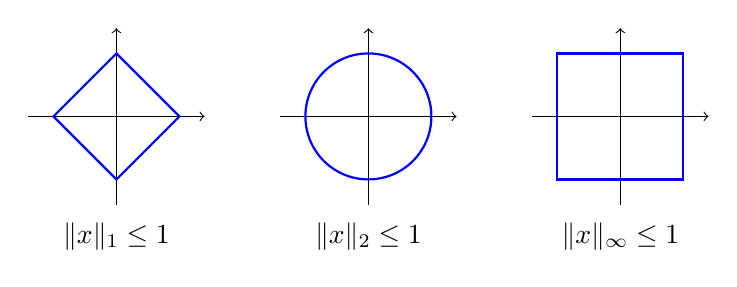
\begin{tikzpicture}[scale=.8]
\foreach \k/\lab in {0/1,4/2,8/\infty}{
\begin{scope}[xshift=\k cm]
\draw[->] (-1.4,0)--(1.4,0); \draw[->] (0,-1.4)--(0,1.4);
\node at (0,-1.9) {$\|x\|_{\lab}\leq1$};
\end{scope}}
\draw[blue,thick] (1,0)--(0,1)--(-1,0)--(0,-1)--cycle;
\draw[blue,thick] (4,0) circle (1);
\draw[blue,thick] (7,-1) rectangle (9,1);
\end{tikzpicture}
\end{center}
Different unit balls do not mean different convergent sequences. The
coordinate comparisons above already show this for the $1$-, $2$-, and
maximum norms.
The following proof follows the same pattern for any norm:
coordinate upper bound, continuity, compact sphere, positive minimum,
then homogeneous rescaling to obtain a lower bound.
\begin{theorem}[Equivalence of norms]
\label{thm:equivalent-norms}
If $V$ is finite dimensional and
\[
\norm{\cdot}_a,\qquad\norm{\cdot}_b
\]
are norms on $V$, then there are $c,C>0$ such that
\[
c\norm v_a\leq\norm v_b\leq C\norm v_a
\]
for every $v\in V$.  Thus the two norms have the same open sets, convergent
and Cauchy sequences, continuous maps, and compact subsets.
\end{theorem}
\begin{proof}
First bound a norm above in coordinates, then obtain a
uniform lower bound on the compact Euclidean sphere. If $V=\{0\}$ any
$c,C>0$ work. Otherwise choose a basis and identify $V$ with $\R^n$.
For any norm on $\R^n$,
\[
\norm{x}_b\leq\sum_{j=1}^{n}\abs{x_j}\norm{e_j}_b
\leq C\norm{x}_2
\]
by Cauchy--Schwarz.  Together with \cref{prop:reverse-triangle}, this gives
\[
\bigl\lvert\norm{x}_b-\norm{y}_b\bigr\rvert
\leq C\norm{x-y}_2,
\]
so $x\mapsto\norm{x}_b$ is Euclidean-continuous.  It has a positive minimum
$c$ on the Euclidean
unit sphere, which is compact by \cref{thm:heine-borel-rn};
\cref{thm:compact-extreme-value} supplies the attained minimum. It is
positive because every sphere point is nonzero. For $x\ne0$, the vector
$u=x/\norm{x}_2$ is on that sphere, so homogeneity gives
$\norm{x}_b=\norm{x}_2\norm{u}_b\geq c\norm{x}_2$; the same inequality
holds at zero. Apply these bounds to each given norm, writing
$c_a\norm{x}_2\leq\norm{x}_a\leq C_a\norm{x}_2$ and
$c_b\norm{x}_2\leq\norm{x}_b\leq C_b\norm{x}_2$. Then
\[
\frac{c_b}{C_a}\norm{x}_a\leq\norm{x}_b
\leq\frac{C_b}{c_a}\norm{x}_a.
\]
Denote the resulting constants by $c,C$. Their ball inclusions are
$B_a(x,\eps/C)\subseteq B_b(x,\eps)$ and
$B_b(x,c\eps)\subseteq B_a(x,\eps)$, so the open sets agree.
Applying the same inequalities to $x_j-x$ and $x_j-x_k$ proves the
convergence and Cauchy assertions. Continuity and compactness agree
because their definitions use only open sets.
\end{proof}

\begin{corollary}[Completeness in finite dimensions]
\label{cor:finite-dimensional-completeness}
Every finite-dimensional normed vector space is complete, and its compact
subsets are exactly its closed bounded subsets.
\end{corollary}
\begin{proof}
Coordinates reduce the assertion to Euclidean space, where completeness
follows coordinatewise from \cref{thm:real-cauchy-complete} and compactness
from \cref{thm:heine-borel-rn}; use \cref{thm:equivalent-norms}.
\end{proof}

Completeness ensures that Cauchy approximations have limits. Chapter~11
uses it to obtain fixed points and solve nonlinear equations.

\section{Operator Norms and Finite-Dimensional Estimates}

A derivative will be a linear map, and its approximation error must be
controlled in every direction at once. We first bound the output by a
constant times the input norm. The operator norm will then record the
smallest such constant and let us measure differences between linear maps.

\begin{proposition}[Finite-dimensional linear maps are Lipschitz]
\label{prop:linear-continuity}
Every linear map $L:V\to W$ between finite-dimensional normed spaces is Lipschitz, hence continuous.
\end{proposition}
\begin{proof}
A bound on the finitely many basis images controls every linear combination.
If $V=\{0\}$ there is nothing to prove. Otherwise choose a basis
$e_1,\ldots,e_n$ of $V$. For $v=\sum_i a_i e_i$ put
$\|v\|_c=\sum_i|a_i|$. Norm equivalence gives $\|v\|_c\leq K\|v\|_V$.
With $M=\max_i\|L(e_i)\|_W$, the triangle inequality gives
\[
\|Lv\|_W\leq\sum_i|a_i|\|L(e_i)\|_W
\leq M\|v\|_c\leq MK\|v\|_V.
\]
Apply this to $v=x-y$ to obtain $\|Lx-Ly\|_W\leq MK\|x-y\|_V$.
No target basis is needed. Finite dimensionality enters through the finite
basis and the norm-equivalence estimate.
\end{proof}
The following characterization does not require finite dimensionality; it
explains which linear maps admit an operator norm. A linear map between
normed spaces is called \textbf{bounded} if
$\|Lv\|_W\leq C\|v\|_V$ for some $C\geq0$ and every $v\in V$.

\begin{theorem}[Bounded linear maps]
\label{thm:bounded-linear-equivalences}
For a linear map $L:V\to W$ between normed spaces, the following are
equivalent:
\[
\begin{aligned}
&L\text{ is continuous};\qquad
L\text{ is continuous at }0;\\
&\exists C\geq0:\ \|Lv\|_W\leq C\|v\|_V\quad(v\in V);\qquad
L\text{ is Lipschitz}.
\end{aligned}
\]
In finite dimensions these conditions hold for every linear map by
\cref{prop:linear-continuity}.
\end{theorem}
\begin{proof}
Continuity implies continuity at zero. If $L$ is continuous at zero, choose
$\delta>0$ such that $\|u\|_V<\delta$ implies $\|Lu\|_W<1$. For
$v\ne0$, apply this to
$u=\delta v/(2\|v\|_V)$ and use linearity to obtain
\[
\|Lv\|_W<\frac{2}{\delta}\|v\|_V.
\]
Consequently the uniform weak inequality
\[
\|Lv\|_W\leq\frac{2}{\delta}\|v\|_V
\qquad(v\in V)
\]
also includes $v=0$. Such a bound applied to $v=x-y$ is the
Lipschitz estimate
$\|Lx-Ly\|_W\leq C\|x-y\|_V$, and every Lipschitz map is continuous.
\end{proof}

\begin{definition}[Operator norm]
For a bounded linear map $L:V\to W$, define
\[
\norm L_{\mathrm{op}}
=\sup\set{\norm{Lv}_W:\norm v_V\leq1}.
\]
Both norms matter; $\|L\|_{V\to W}$ makes their roles visible.
\end{definition}

\Needspace{18\baselineskip}
\begin{theorem}[Characterizations of the operator norm]
\label{thm:operator-norm-characterizations}
Let $V\ne\{0\}$ and let $L:V\to W$ be bounded and linear. Then
\[
\boxed{
\begin{aligned}
\|L\|_{\mathrm{op}}
&=\sup_{\|v\|_V\leq1}\|Lv\|_W
=\sup_{\|v\|_V=1}\|Lv\|_W\\
&=\sup_{v\ne0}\frac{\|Lv\|_W}{\|v\|_V}
=\sup_{x\ne y}\frac{\|Lx-Ly\|_W}{\|x-y\|_V}\\
&=\inf\left\{C\geq0:
\|Lv\|_W\leq C\|v\|_V\text{ for every }v\in V\right\}.
\end{aligned}}
\]
Thus the operator norm is the optimal Lipschitz constant of a linear map.
If $V$ is finite dimensional, then
\[
\|L\|_{\mathrm{op}}=\max_{\|v\|_V=1}\|Lv\|_W.
\]
\end{theorem}
\begin{proof}
For every $v\ne0$, normalize it by
\[
u=\frac{v}{\|v\|_V},\qquad \|u\|_V=1.
\]
Linearity gives
\[
\frac{\|Lv\|_W}{\|v\|_V}=\|Lu\|_W.
\]
This proves equality of the unit-sphere and nonzero-vector suprema. It also
shows that every vector in the closed unit ball contributes at most the
unit-sphere supremum, while the sphere is contained in that ball. Hence the
first three suprema agree and
\[
\|Lv\|_W\leq\|L\|_{\mathrm{op}}\|v\|_V.
\]
Conversely, every constant $C$ satisfying this inequality bounds the unit-ball
supremum, so $\|L\|_{\mathrm{op}}\leq C$. The operator norm itself is one
such bound, proving the infimum formula.

Since $Lx-Ly=L(x-y)$, every difference quotient is one of the nonzero-vector
ratios. Conversely every nonzero $v$ occurs as $x-y$ by taking $x=v$ and
$y=0$. This proves the Lipschitz formula and its optimality.

In finite dimensions the unit sphere is closed and bounded, hence compact by
\cref{cor:finite-dimensional-completeness}. The function
$v\mapsto\|Lv\|_W$ is continuous by
\cref{thm:bounded-linear-equivalences,prop:reverse-triangle}; therefore
\cref{thm:compact-extreme-value} turns its supremum into a maximum.
\end{proof}

An upper estimate proves only $\|L\|\leq C$; an input attaining $C$
proves equality. The coefficient bound $(\sum_{i,j}a_{ij}^2)^{1/2}$
is generally only an upper bound: for the Euclidean identity on $\R^2$
it is $\sqrt2$, whereas the operator norm is $1$.
\begin{proposition}[Operator-norm estimates]
\label{prop:operator-norm-estimates}
The operator norm is a norm on the vector space of bounded linear maps
$V\to W$. In finite dimensions every linear map is bounded, so it is a
norm on $\mathcal L(V,W)$. For bounded maps $L:V\to W$ and $S:W\to Z$,
\[
\|S\circ L\|_{\mathrm{op}}
\leq\|S\|_{\mathrm{op}}\|L\|_{\mathrm{op}}.
\]
\end{proposition}
\begin{proof}
Homogeneity and the triangle inequality follow pointwise and then by taking
suprema. If the norm is zero, the displayed bound gives $Lv=0$ for every
$v$, so $L=0$. Finally
$\|(S\circ L)v\|\leq\|S\|_{\mathrm{op}}\|L\|_{\mathrm{op}}\|v\|$;
take the supremum over $\|v\|\leq1$.
\end{proof}



The estimate $\norm{T(v)}\leq C\norm v$ says quantitatively that a linear
map cannot amplify a small input error without bound.  Every
finite-dimensional linear map has such a bound; this is the prototype for
the operator-norm estimates on derivatives used later.

\begin{example}[A diagonal operator norm]
For $L(x,y)=(3x,-2y)$ in Euclidean norm,
\[
\norm{L(x,y)}_2^2=9x^2+4y^2\leq9(x^2+y^2).
\]
Equality on $(1,0)$ proves $\norm L_{\mathrm{op}}=3$.
More generally a diagonal map has Euclidean operator norm
$\max_i|a_{ii}|$, by the same bound and a maximizing coordinate vector.
\end{example}
\begin{example}[An operator norm depends on the chosen lengths]
Let $T(x,y)=(x+2y,0)$. With the max norm on both spaces,
\[
\|T(x,y)\|_\infty=|x+2y|\leq3\|(x,y)\|_\infty.
\]
The max-unit vector $(1,1)$ attains $3$, so
$\|T\|_{\infty\to\infty}=3$. With the sum norm on both spaces,
\[
\|T(x,y)\|_1=|x+2y|\leq|x|+2|y|\leq2\|(x,y)\|_1.
\]
The sum-unit vector $(0,1)$ attains $2$, so $\|T\|_{1\to1}=2$.
The map is unchanged but the exact norms differ. An upper bound alone is
not automatically the exact operator norm: equality requires an input
attaining the bound, or inputs approaching it.
\end{example}
\begin{example}[An estimate transferred to a polynomial space]
On $P_2$ use the coefficient norm
$\|a+bt+ct^2\|_c=|a|+|b|+|c|$, and on $P_1$ use the analogous
norm. Differentiation satisfies
$\|D(a+bt+ct^2)\|_c=|b|+2|c|\leq2\|a+bt+ct^2\|_c$.
Equality at $t^2$ gives operator norm $2$. If the spaces instead use
the integral inner-product norms, this number need not remain $2$, but
norm equivalence still guarantees a finite bound. The intrinsic map has
not changed, while a numerical error-amplification constant depends on
how the two spaces measure error.
\end{example}

Composition means successive amplification: $L$ amplifies by at most
$\|L\|$, then $S$ by at most $\|S\|$. This explains the product bound.
In Chapter~11 the approximation $f(a+h)=f(a)+Df(a)h+o(\|h\|)$ uses
$\|Df(a)h\|\leq\|Df(a)\|_{\mathrm{op}}\|h\|$.
For $\lambda(h)=c\cdot h$ on Euclidean $\R^n$, with absolute value on
the scalar target, $\|\lambda\|_{\mathrm{op}}=\|c\|_2$: Cauchy--Schwarz
gives the upper bound and $h=c/\|c\|_2$ attains it when $c\ne0$.
The zero case is immediate. Chapter~11 will apply this to scalar derivatives.
For example $\lambda(x,y)=3x-4y$ has norm $5$, attained at $(3/5,-4/5)$.

\subsection{Series of vectors and operators}
A series $\sum_{k=0}^\infty v_k$ in a finite-dimensional normed space $V$
means the limit of its partial sums. Norm equivalence shows that convergence
is equivalent to convergence of every coordinate series in any basis.
If $\sum_k\|v_k\|<\infty$, the estimate
$\|\sum_{k=p}^qv_k\|\leq\sum_{k=p}^q\|v_k\|$ makes partial sums Cauchy;
finite-dimensional completeness supplies their limit. For a linear map
$L:V\to W$, continuity applied to partial sums gives
$L(\sum_kv_k)=\sum_kL(v_k)$. Scalar convergence tests need no redevelopment.
\begin{proposition}[Operator geometric series]\label{prop:neumann-series}
For $T\in\mathcal L(V)$ with $\|T\|_{\mathrm{op}}<1$,
\[
(I-T)^{-1}=\sum_{k=0}^\infty T^k
\]
with convergence in operator norm.
\end{proposition}
\begin{proof}
The space $\mathcal L(V)$ is finite dimensional (its basis coordinates
are the finitely many matrix entries). Since $\|T^k\|\leq\|T\|^k$
for $k\geq1$, absolute convergence follows from the scalar geometric series.
For $S_N=\sum_{k=0}^NT^k$, direct cancellation gives
$(I-T)S_N=S_N(I-T)=I-T^{N+1}$. Pass to the limit using the composition
estimate; both products equal $I$. This also covers the zero space.
\end{proof}
\section{Dual Spaces and Multilinear Maps}
\label{sec:dual-multilinear}
A scalar-valued derivative measures how a direction changes a scalar
output. This calls for a linear functional, rather than another direction.
\begin{definition}[Covectors and the dual space]\label{def:covector-dual}
A \textbf{linear functional}, or \textbf{covector}, on a real vector space
$V$ is a linear map $\lambda:V\to\R$. The \textbf{dual space} is
$V^*=\mathcal L(V,\R)$, with pointwise addition and scalar multiplication.
\[
v\in V\quad\text{(vector)},\qquad
\lambda\in V^*\quad\text{(covector)},\qquad
\lambda(v)\in\R\quad\text{(scalar)}.
\]
A vector represents a direction or displacement; a covector evaluates on a
vector and returns a scalar. Thus scalar-valued derivatives naturally
produce covectors.
\end{definition}
\begin{definition}[Kronecker delta and dual basis]\label{def:dual-basis}
The \textbf{Kronecker delta} is
\[
\delta^i_j=\begin{cases}1,&i=j,\\0,&i\ne j.\end{cases}
\]
Thus $(\delta^i_j)$ is the identity matrix written entrywise.
For an ordered basis $\mathcal B=(e_1,\ldots,e_n)$ of $V$, its
\textbf{dual basis} is the unique family
$\mathcal B^*=(e^1,\ldots,e^n)$ in $V^*$ satisfying
$e^i(e_j)=\delta^i_j$.
\end{definition}
Here are existence, uniqueness, and the reason it is a basis. Define
$e^i(\sum_j v^j e_j)=v^i$. Unique vector coordinates make this well defined;
coordinates of sums and scalar multiples show it is linear. Any covector
with the prescribed values on $e_j$ must have these same values on every
linear combination, proving uniqueness. For any $\lambda\in V^*$,
\[
\boxed{v=\sum_i e^i(v)e_i,\qquad
\lambda=\sum_i\lambda(e_i)e^i.}
\]
The second equality holds on each $e_j$, hence on every vector by linearity.
Evaluating a relation $\sum_i c_i e^i=0$ on $e_j$ gives $c_j=0$.
Thus the $e^i$ span $V^*$ independently, and $\dim V^*=n$.
The $e_i$ build vectors from coordinates; the $e^i$ extract coordinates.
Subscripts label vectors and superscripts label covectors, not powers.
Chapter~11 identifies the standard dual basis with coordinate differentials
$\dd x_i$ by differentiating coordinate projections.
For example, $\lambda=2e^1-e^2$ evaluates on $(3,4)$ as $2$.
Its coordinate row is $(2,-1)$, whereas a vector's coordinate column has
a different role. A column and a row represent these objects after bases
are chosen; they do not intrinsically identify a vector with a covector.
For scalar-valued $f$ in Chapter~11, $Df(a)\in V^*$.
Its Euclidean vector representative is $\nabla f(a)$, determined by
$Df(a)h=\nabla f(a)\cdot h$.

\begin{example}[Classical planes and covectors]\label{ex:affine-hyperplane}
For $0\ne\lambda\in V^*$, the equation $\lambda(x)=c$ defines an
\textbf{affine hyperplane}. Choose $p$ with $\lambda(p)=c$: if
$\lambda(v)\ne0$, take $p=cv/\lambda(v)$. Linearity gives
\[
\{x:\lambda(x)=c\}=p+\ker\lambda.
\]
The direction space is $\ker\lambda$, of codimension one by rank--nullity;
the affine set itself need not contain zero. In $\R^3$ this connects a
Cartesian equation $ax+by+cz=d$ with $p+\operatorname{span}(u,v)$.
For example, for $2x-y+3z=5$ take
\[
p=(1,0,1),\quad u=(1,2,0),\quad v=(0,3,1),\qquad
\lambda=2\,\dd x-\dd y+3\,\dd z.
\]
Here $\dd x,\dd y,\dd z$ denote the standard coordinate covectors, and
$\ker\lambda=\{(u_1,u_2,u_3):2u_1-u_2+3u_3=0\}$.
With the Euclidean inner product the normal is $n=(2,-1,3)$, since
$\lambda(w)=n\cdot w$. The covector is defined without an inner product;
its representing normal vector depends on that additional choice.
\end{example}
% Original vector figure for Version 3.9.0.
\begin{figure}[htbp]
\centering
\begin{tikzpicture}[font=\small,>=Stealth,line width=.65pt]
\filldraw[fill=gray!8,draw=gray] (-2,-1.3)--(.6,-1.3)--(1.8,-.6)--(-.8,-.6)--cycle;
\node[below] at (-.1,-1.3) {$\ker\lambda$};
\fill (0,-.9) circle(1.5pt) node[left] {$0$};
\filldraw[fill=blue!9,draw=blue!70!black] (-2,.2)--(.6,.2)--(1.8,.9)--(-.8,.9)--cycle;
\coordinate (p) at (0,.6);\fill (p) circle(2pt) node[below] {$p$};
\draw[->,blue!80!black,thick] (p)--(1,.6) node[right] {$u$};
\draw[->,blue!80!black,thick] (p)--(.65,.98) node[above right] {$v$};
\draw[->,red!75!black,thick] (p)--(0,2) node[above] {$n$};
\draw[dashed,gray] (0,-.9)--(p);
\node[right,align=left] at (2,.5) {$p+\ker\lambda$\\$\lambda(x)=c$};
\end{tikzpicture}
\caption{An affine plane and its parallel direction plane. The arrows $u,v$ span the direction space; a Euclidean normal $n$ represents the covector. Orthogonality is spatial, not an angle measured on this oblique drawing.}\label{fig:affine-hyperplane}
\end{figure}

\begin{example}[Finding a dual basis, rather than guessing it]
For $b_1=(1,1),b_2=(1,-1)$, seek $b^1(x,y)=ax+by$ satisfying
$a+b=1$ and $a-b=0$. Thus $b^1(x,y)=(x+y)/2$.
Similarly $b^2(x,y)=(x-y)/2$. Each extracts the coefficient of
its own basis vector: $(x,y)=b^1(x,y)b_1+b^2(x,y)b_2$.
For $\lambda(x,y)=3x-y$, its values on $b_1,b_2$ are $2,4$, so
$\lambda=2b^1+4b^2$. The coordinate row changes from $(3,-1)$ to
$(2,4)$ while the functional stays fixed.
\end{example}
The gradient is an inner-product representative, not the covector itself.
For example the functional $\lambda(x,y)=x$ is represented by $(1,0)$
for the usual dot product, but by $(1/2,0)$ for
$\langle u,v\rangle=2u_1v_1+u_2v_2$. Both pairings return $x$.
No such choice is needed to evaluate $\lambda$ or to pull it back.
\begin{definition}[Pullback of a covector]\label{def:covector-pullback}
For linear $T:V\to W$, define $T^*:W^*\to V^*$ by
$T^*(\lambda)=\lambda\circ T$. Vectors are sent forward by $T$;
covectors are pulled back by composition. This map is linear because
composition distributes over sums and scalar multiples of functionals.
\end{definition}
For $T(x,y)=(x+2y,3y)$ and $\lambda(u,v)=2u-v$, one obtains
$T^*\lambda(x,y)=2x+y$. In coordinates the row $(2,-1)$ is multiplied
on the right by the matrix of $T$.

\begin{definition}[Multilinear maps]
A map $A:V_1\times\cdots\times V_k\to W$ is $k$-multilinear if each
slot $r$ satisfies the following conditions, with all other inputs fixed:
\begin{align*}
A(\ldots,u+v,\ldots)&=A(\ldots,u,\ldots)+A(\ldots,v,\ldots),\\
A(\ldots,au,\ldots)&=aA(\ldots,u,\ldots).
\end{align*}
The vectors $u,v$ belong to $V_r$ and $a\in\R$. For $k=2$ the map is
called bilinear. A single scaling of the whole input tuple is not the
condition; one input varies at a time.
\end{definition}
Examples are $x\cdot y$, $x^{\mathsf T}Ay$ for a fixed matrix $A$, and
the signed-area expression $v_1w_2-v_2w_1$ in the plane. A bilinear map
is generally \emph{not} linear on the product vector space:
$B(2x,2y)=4B(x,y)$, whereas product-space linearity would require
$2B(x,y)$. Ordinary multiplication $B(x,y)=xy$ already demonstrates this.

Expanding one argument at a time shows that a multilinear map is determined
by its values on tuples of basis vectors. In the bilinear case,
\[
B\left(\sum_i x_ie_i,\sum_j y_jf_j\right)
=\sum_i\sum_j x_iy_jB(e_i,f_j).
\]
Repeating this for $k$ slots gives a sum of products of $k$ coordinates
times the corresponding basis-tuple value. If all $V_j$ and $W$ are
finite dimensional, this identifies the map space with a finite collection
of $W$-valued basis data, so the map space is finite dimensional. The
logical chain is: basis values determine the map, the finite expansion
gives a norm estimate, and the estimate gives continuity.
In finite-dimensional normed spaces every
multilinear map is bounded: coordinate bounds and the triangle inequality
give a constant $C$ such that
$\norm{A(v_1,\ldots,v_k)}\leq C\prod_j\norm{v_j}$.
For bilinear maps, for example, bound each $|x_i|$ and $|y_j|$ by fixed
multiples of $\norm x$ and $\norm y$ and sum the finitely many
$\norm{B(e_i,f_j)}$. This bound also proves continuity, by telescoping
the difference of two evaluations one slot at a time.

\begin{example}[Basis values and a complete bilinear estimate]
On $\R^2$, suppose $B(e_1,e_1)=1$, $B(e_1,e_2)=2$,
$B(e_2,e_1)=-1$, and $B(e_2,e_2)=3$. Then
\[
B(x,y)=x_1y_1+2x_1y_2-x_2y_1+3x_2y_2.
\]
The four basis values force this expression. Since every coordinate
magnitude is at most the Euclidean norm,
$|B(x,y)|\leq7\|x\|_2\|y\|_2$. This is an upper bound, not a
claim that $7$ is optimal. To compare nearby input pairs, write the
exact two-slot telescoping identity
\[
B(x,y)-B(x',y')=B(x-x',y)+B(x',y-y').
\]
Near a fixed pair the factors $\|y\|$ and $\|x'\|$ stay bounded,
so the displayed estimate proves continuity. For more slots replace
one argument at a time and add the resulting differences. We will use
this estimate for higher derivatives.
\end{example}

\begin{definition}[Alternating maps]
An alternating $k$-multilinear map $A:V^k\to W$ is one that vanishes
whenever two arguments are equal:
\[
v_i=v_j\text{ for some }i\ne j\quad\Longrightarrow\quad A(v_1,\ldots,v_k)=0.
\]
The repeated-argument-zero condition is
the definition; a sign rule will be a consequence.
\end{definition}
\Needspace{8\baselineskip}
\begin{proposition}[Alternation]
\label{prop:alternation}
Swapping two arguments of an alternating map changes its sign. An
alternating map vanishes on linearly dependent arguments.
\end{proposition}
\begin{proof}
Put $u+v$ in the two slots and expand the value $0$. The terms with two
$u$'s or two $v$'s vanish, leaving $A(\ldots,u,\ldots,v,\ldots)
+A(\ldots,v,\ldots,u,\ldots)=0$. For dependent arguments, express one
as a combination of the others; every term then repeats an argument.
A zero argument gives zero directly by linearity, including the one-slot case.
\end{proof}

\begin{proposition}[Norm-valued remainder rules]
\label{prop:norm-remainder-rules}
As $h\to0$, sums of $O(\norm h)$ terms remain $O(\norm h)$ and sums of
$o(\norm h)$ terms remain $o(\norm h)$. If $L$ is bounded linear and
$r(h)=o(\norm h)$, then $Lr(h)=o(\norm h)$. If
$k(h)=O(\norm h)$ and $r(k)=o(\norm k)$ with $r(0)=0$, then
$r(k(h))=o(\norm h)$, whenever the composition is defined near $0$.
For bounded bilinear $B$, if $u(h),v(h)=O(\norm h)$, then
$B(u(h),v(h))=O(\norm h^2)=o(\norm h)$.
\end{proposition}
\begin{proof}
Replace the symbols by norm inequalities, including the case
of a zero intermediate increment. Triangle inequalities prove the sum
rules. The bound $\norm{Lr(h)}\leq\norm L_{\mathrm{op}}\norm{r(h)}$
proves the linear rule after division by $\norm h$.
For composition, choose $C\geq1$ with $\norm{k(h)}\leq C\norm h$.
Given $\eps>0$, the estimate $\norm{r(k)}\leq(\eps/C)\norm k$
holds for sufficiently small nonzero $k$, and for $k=0$ because $r(0)=0$.
Since $k(h)\to0$, it gives $\norm{r(k(h))}\leq\eps\norm h$ eventually.
Finally the bilinear bound gives
$\norm{B(u(h),v(h))}\leq C_B C_u C_v\norm h^2$; division by
$\norm h$ makes this tend to zero.
\end{proof}
The condition $r(0)=0$ is essential if $k(h)$ sometimes vanishes; the
punctured little-o statement alone imposes no value at zero. Derivative
remainders have this value by their definition. These estimates justify
the product and chain-rule manipulations in Chapter~11.

\section{Determinants and Orientation}
\label{sec:determinants}
In $\R^2$, $v_1w_2-v_2w_1$ measures the signed area of the ordered
parallelogram spanned by $v,w$. Doubling one side doubles it; replacing
a side by a sum adds the signed contributions; equal sides give zero.
The standard ordered unit square has value $1$. These suggest three
properties of signed volume in higher dimensions: multilinearity,
alternation, and normalization on the standard basis. Volume magnitude
and orientation sign are related but distinct; Chapter~12 proves the
precise volume-scaling theorem.

\begin{definition}[Normalized determinant form]
A normalized determinant form on $\R^n$ is an alternating $n$-linear
scalar-valued map whose value on $(e_1,\ldots,e_n)$ is $1$.
\end{definition}
The sign-change lemma is \cref{prop:alternation}: putting $u+v$ in
two slots and expanding its four terms proves the minus sign for an
interchange. This lemma supplies the effect of a swap on a form; the
elementary parity facts supply how the signs of successive swaps combine.
It remains to show that the structural requirements are consistent and
determine exactly one form.

\subsection*{The permutation signs needed here}

Multilinear expansion will produce terms indexed by reorderings of basis
vectors. Alternation requires a sign for each reordering. Counting inverted
pairs gives a sign directly from the permutation, without choosing a
possibly nonunique sequence of swaps.

A permutation is a bijection of $\{1,\ldots,n\}$ to itself; $S_n$ is
their set, with $(\sigma\tau)(j)=\sigma(\tau(j))$. Define
\[
\operatorname{inv}(\sigma)=\#\{(i,j):i<j,\ \sigma(i)>\sigma(j)\},\qquad
\operatorname{sgn}(\sigma)=(-1)^{\operatorname{inv}(\sigma)}.
\]
\begin{proposition}[Sign rules]\label{prop:permutation-sign}
Swapping two entries reverses sign, and
\[
\operatorname{sgn}(\sigma\tau)=\operatorname{sgn}(\sigma)\operatorname{sgn}(\tau),
\qquad \operatorname{sgn}(\sigma^{-1})=\operatorname{sgn}(\sigma).
\]
\end{proposition}
\begin{proof}
Swapping adjacent entries changes only their mutual inversion: comparisons
with each outside entry have the same total before and after. Thus it
reverses sign. Swapping positions $p<q$ can be done by moving the first
entry right through $q-p$ adjacent swaps, then the other left through
$q-p-1$ swaps. The odd total $2(q-p)-1$ reverses sign.
Repeatedly swap an adjacent inverted pair. Each step reduces the inversion
number by one; a list with none is the increasing identity list. Reversing
these steps expresses $\tau$ by $\operatorname{inv}(\tau)$ adjacent swaps.
Apply the same position swaps to the list for $\sigma$. The final list is
$(\sigma(\tau(1)),\ldots,\sigma(\tau(n)))$, so its sign changes by
$(-1)^{\operatorname{inv}(\tau)}$. This proves multiplicativity.
Apply it to $\sigma\sigma^{-1}$ to prove the inverse identity.
\end{proof}

\begin{theorem}[The normalized determinant form]
\label{thm:determinant-form}
There is a unique alternating $n$-linear map
$\det:(\R^n)^n\to\R$ with $\det(e_1,\ldots,e_n)=1$.
More generally, every alternating $n$-linear form $F$ on $\R^n$ is
determined by its one value $c=F(e_1,\ldots,e_n)$ and satisfies $F=c\det$.
\end{theorem}
\begin{proof}
Expand basis coordinates one slot at a time. Alternation
removes repeated choices; the remaining basis tuples can be reordered
to the standard one. We separate uniqueness from existence.
Write $x_j=\sum_i a_{ij}e_i$.
The slot number $j$ specifies which input is being expanded. The index
$i$ specifies which standard basis vector occurs in that input. Thus
$a_{ij}$ lies in row $i$, column $j$ of the matrix of input columns.
The separate indices $i_1,i_2,\ldots$ below are independent choices:
$i_2$ is not constrained by the choice already made for $i_1$. Expanding the first slot gives
\[
F(x_1,x_2,\ldots,x_n)=\sum_{i_1=1}^n a_{i_1,1}F(e_{i_1},x_2,\ldots,x_n).
\]
For $n\geq2$, expand the second slot of \emph{each} resulting term:
\[
F(x_1,\ldots,x_n)=\sum_{i_1=1}^n\sum_{i_2=1}^n
a_{i_1,1}a_{i_2,2}F(e_{i_1},e_{i_2},x_3,\ldots,x_n).
\]
Continuing through all slots gives
\[
F(x_1,\ldots,x_n)=\sum_{i_1,\ldots,i_n=1}^n
a_{i_1,1}\cdots a_{i_n,n}F(e_{i_1},\ldots,e_{i_n}).
\]
Each term chooses one basis vector from each input, with the product of
the chosen coefficients. There are $n^n$ choices. Terms with repeated
indices vanish. In each remaining term every index occurs once, and a
sequence of swaps puts the arguments into $(e_1,\ldots,e_n)$, determining
its value from $c$. Thus two forms with the same $c$ agree on every tuple.
A multi-index $(i_1,\ldots,i_n)$ records one such choice for every
slot. If $i_r=i_s$, the basis tuple repeats a vector, so alternation
kills that whole term even if its coefficient is nonzero. Without
repetitions, $n$ choices from $n$ labels use every label exactly once:
these are exactly the $n!$ permutations. Multilinearity produces all
choices; alternation removes repeated choices; permutations are exactly
the choices that remain.

A surviving tuple defines the permutation $\sigma(j)=i_j$. Therefore
\[
F(e_{i_1},\ldots,e_{i_n})
=F(e_{\sigma(1)},\ldots,e_{\sigma(n)})
=\operatorname{sgn}(\sigma)F(e_1,\ldots,e_n).
\]
Reordering each surviving tuple contributes its sign, so necessarily
\[
F(x_1,\ldots,x_n)=c\sum_{\sigma\in S_n}\operatorname{sgn}(\sigma)
\prod_{j=1}^n a_{\sigma(j),j}.
\]
For existence define the determinant by this Leibniz sum with $c=1$.
The constructed
expression is linear in each column of coordinates. When two inputs agree,
say columns $r,s$, pair the permutations by
\[
\sigma\longleftrightarrow\sigma\circ(r\ s).
\]
Applying this pairing twice returns $\sigma$, and it has no fixed point
because $\sigma(r)\ne\sigma(s)$. Equal columns give explicitly
\[
a_{\sigma(r),r}a_{\sigma(s),s}
=a_{\sigma(r),s}a_{\sigma(s),r},\qquad
\operatorname{sgn}(\sigma\circ(r\ s))=-\operatorname{sgn}(\sigma).
\]
All remaining factors are unchanged. Each pair therefore sums to zero. Thus the expression is alternating. On the standard
basis only the identity choice remains and has value $1$.
This proves existence. The same uniqueness argument applied to $F$ and
$c\det$ proves the final assertion, including $c=0$.
\end{proof}
\begin{remark}[A fuller permutation discussion]
The treatment here is deliberately streamlined toward the determinant and
is self-contained. Appendix~\ref{app:determinants} develops cycles,
transpositions, adjacent swaps, inversion counting, parity, and permutation
matrices more slowly. Readers wanting concrete practice may read that
supplementary material before continuing.
\end{remark}

\begin{remark}[Why this proof has so many indices]
This first complete multilinear expansion is unusually index-heavy because
every input is simultaneously expressed in a basis. Later arguments may
say ``expand by multilinearity'' after identifying the slots being expanded;
they usually work directly with the given vectors and do not need this full
bookkeeping. The underlying operation is always the same distribution of
one sum at a time.
\end{remark}
\begin{example}[From 27 choices to six]
For $n=3$, expand in terms
$a_{i1}a_{j2}a_{k3}F(e_i,e_j,e_k)$ for $1\leq i,j,k\leq3$.
The term $(1,1,2)$ vanishes. The choices $(1,2,3)$ and $(2,1,3)$
contribute $a_{11}a_{22}a_{33}c$ and $-a_{21}a_{12}a_{33}c$.
Of the $27$ formal terms, only the six orderings of $(1,2,3)$ can survive;
some of these may still have zero coefficients. The calculation uses
multilinearity and alternation alone.
\end{example}
For a square matrix $A$ with columns $A_1,\ldots,A_n$, define
$\det A=\det(A_1,\ldots,A_n)$. The preceding proof adapts the
slot-by-slot argument in the author's algebra notes, Theorem~5.12.3.

\begin{theorem}[Determinant laws]
\label{thm:determinant-properties}
Swapping columns negates the determinant, scaling a column scales it by
the same factor, and adding a multiple of another column leaves it unchanged.
Dependent columns give zero. Moreover
\[
\det I_n=1,\qquad\det(AB)=\det A\det B,\qquad
\det A\ne0\ \Longleftrightarrow\ A\text{ is invertible}.
\]
An upper or lower triangular matrix has determinant $\prod_i a_{ii}$.
\end{theorem}
\begin{proof}
Use alternation for column operations and uniqueness for
composition. Scaling is multilinearity; swaps and dependent columns were
proved in \cref{prop:alternation}. Adding $cA_i$ to a different column
adds a determinant with two equal columns, which is zero.
To measure what a fixed map $A$ does to every parallelepiped, feed
its transformed edge vectors into the volume form. Define
\[
F(v_1,\ldots,v_n)=\det(Av_1,\ldots,Av_n).
\]
For any slot, $A(av+bw)=aAv+bAw$ followed by determinant multilinearity
proves linearity there; equal inputs have equal images, proving alternation.
Its value at the standard basis is $\det A$. The normalized determinant
theorem therefore compares the two alternating forms $F$ and
$(\det A)\det$, which have the same value on that basis, and gives
\[
\det(Av_1,\ldots,Av_n)=(\det A)\det(v_1,\ldots,v_n).
\]
Matrix multiplication gives $AB=[AB_1\ \cdots\ AB_n]$, so
\[
\begin{aligned}
\det(AB)&=\det(AB_1,\ldots,AB_n)\\
&=(\det A)\det(B_1,\ldots,B_n)=(\det A)(\det B).
\end{aligned}
\]
If $A$ is invertible, $1=\det(AA^{-1})=\det A\det A^{-1}$.
If it is not, its columns are dependent by the basis and bijectivity
criteria, so its determinant is zero.
For upper triangular $A$, the first column is $a_{11}e_1$.
In the expansion of column two only $a_{22}e_2$ can survive, since the
$e_1$ choice repeats. For $n\geq2$ the first two stages are
\[
\begin{aligned}
\det A&=a_{11}\det(e_1,a_{12}e_1+a_{22}e_2,A_3,\ldots,A_n)\\
&=a_{11}a_{12}\det(e_1,e_1,A_3,\ldots,A_n)
+a_{11}a_{22}\det(e_1,e_2,A_3,\ldots,A_n)\\
&=a_{11}a_{22}\det(e_1,e_2,A_3,\ldots,A_n).
\end{aligned}
\]
At stage $j$, the choices $e_1,\ldots,e_{j-1}$ all repeat a previous
input; only $a_{jj}e_j$ survives. Induction yields
$\det A=(\prod_j a_{jj})\det(e_1,\ldots,e_n)=\prod_j a_{jj}$.
The case $n=1$ is just scaling. For lower triangular matrices run this argument
from the last column to the first.
\end{proof}

\begin{proposition}[Rank and nonzero minors]\label{prop:rank-minors}
An $r\times r$ \textbf{minor} of an $m\times n$ matrix $A$ is the
determinant of the square submatrix selected by $r$ rows and $r$ columns,
in their original order. For $0\leq r\leq\min(m,n)$,
\[
\operatorname{rank}A\geq r
\quad\Longleftrightarrow\quad
\text{some $r\times r$ minor is nonzero}.
\]
Thus the rank is the largest size of a nonzero minor, with the empty
$0\times0$ determinant taken to be $1$.
\end{proposition}
\begin{proof}
The assertion for $r=0$ follows from the empty-determinant convention.
If the rank is at least $r>0$, choose $r$ independent columns and form
the corresponding $m\times r$ matrix $B$. Its rows span $\R^r$:
otherwise a basis of their span has $s<r$ elements, and the map taking
a vector to its scalar products with these $s$ rows has a nonzero kernel
by \cref{thm:rank-nullity}. A nonzero vector in that kernel is annihilated
by every row of $B$, contrary to the independence of its columns.
Choose $r$ independent rows of $B$. The resulting square matrix has
zero kernel, since its rows span $\R^r$, and hence is invertible.
By \cref{thm:determinant-properties} its determinant is nonzero.
Conversely, a nonzero $r\times r$ minor gives an invertible submatrix.
Any relation among the corresponding columns of $A$, restricted to the
selected rows, therefore has all coefficients zero. Those columns are
independent, so $\operatorname{rank}A\geq r$.
\end{proof}

\subsection*{The coordinate formula follows from the structure}
The determinant proof now reads as the forced \textbf{Leibniz formula}:
\[
\det A=\sum_{\sigma\in S_n}\operatorname{sgn}(\sigma)
\prod_{j=1}^n a_{\sigma(j),j}.
\]
Multilinearity produces all choices; alternation removes repeated choices;
permutations are exactly the choices that remain. Each product uses one
entry from each column and each row. For
$\left(\begin{matrix}a&b&c\\d&e&f\\g&h&i\end{matrix}\right)$
the six terms are
\[
aei+bfg+cdh-ceg-bdi-afh.
\]

\Needspace{18\baselineskip}
\begin{example}[The six Leibniz terms]
In the table, the list is $(\sigma(1),\sigma(2),\sigma(3))$.
It selects one row in column one, one in column two, and one in column
three. Use the matrix
\[
A=\begin{pmatrix}a&b&c\\d&e&f\\g&h&i\end{pmatrix}.
\]
\begin{center}
\begin{tabular}{cclcc}
list & parity/sign & selected positions & product & contribution\\\hline
$123$ & even/$+$ & $(1,1),(2,2),(3,3)$ & $aei$ & $+aei$\\
$132$ & odd/$-$ & $(1,1),(3,2),(2,3)$ & $ahf$ & $-ahf$\\
$213$ & odd/$-$ & $(2,1),(1,2),(3,3)$ & $dbi$ & $-dbi$\\
$231$ & even/$+$ & $(2,1),(3,2),(1,3)$ & $dhc$ & $+dhc$\\
$312$ & even/$+$ & $(3,1),(1,2),(2,3)$ & $gbf$ & $+gbf$\\
$321$ & odd/$-$ & $(3,1),(2,2),(1,3)$ & $gec$ & $-gec$
\end{tabular}
\end{center}
For $\left(\begin{matrix}1&2&3\\2&5&8\\1&3&6\end{matrix}\right)$
the six contributions in this order are $30,-24,-24,18,16,-15$.
Their sum is $1$. Only for three-by-three matrices does this short
six-term mnemonic apply; a four-by-four determinant has $24$ terms.
\end{example}
\begin{proposition}[Transpose and intrinsic determinant]
\label{prop:transpose-intrinsic-det}
The transpose $A^{\mathsf T}$, obtained by exchanging rows and columns,
has the same determinant as $A$. For an endomorphism $T:V\to V$,
$\det[T]_{\mathcal B}$ is independent of the basis $\mathcal B$;
we may therefore denote this scalar by $\det T$.
\end{proposition}
\begin{proof}
The reindexing $i=\sigma(j)$ gives
\[
\begin{aligned}
\det(A^{\mathsf T})
&=\sum_{\sigma\in S_n}\operatorname{sgn}(\sigma)\prod_j a_{j,\sigma(j)}\\
&=\sum_{\sigma\in S_n}\operatorname{sgn}(\sigma^{-1})
\prod_i a_{\sigma^{-1}(i),i}=\det A.
\end{aligned}
\]
Inversion is a bijection of $S_n$ preserving sign, so the last sum is
exactly the Leibniz sum. If $P$ expresses the new basis in the old one,
the new matrix is $P^{-1}[T]_{\mathcal B}P$. Therefore
\[
\det(P^{-1}[T]_{\mathcal B}P)
=(\det P)^{-1}\det[T]_{\mathcal B}\det P=\det[T]_{\mathcal B}.
\]
This proves that the scalar is independent of coordinates.
\end{proof}
Transpose invariance gives all the column rules for rows as well.
In particular, interchanging two rows changes the determinant's sign,
multiplying a row by $c$ multiplies the determinant by $c$, and adding
$c$ times a different row leaves it unchanged. For the last assertion,
row multilinearity splits the new determinant into the original one and
$c$ times a determinant with two equal rows; the latter vanishes.
These are consequences of the determinant's construction and transpose
invariance, so row reduction can now be used to compute it.

For maps between different spaces a determinant requires choices of volume
normalizations; a scalar independent of both bases is not asserted.
Appendix~\ref{app:tensors}, \cref{thm:top-exterior-determinant}, gives a
retrospective fourth characterization: the induced action on the top
exterior power multiplies by this same scalar. Its four-viewpoint synthesis
connects normalized alternation, Leibniz, recursive Laplace expansion, and
top exterior action without replacing the proofs here.

\subsection*{Minors, cofactors, and efficient computation}
The structural laws are best for theory. Jacobians also require actual
numbers, and cofactor expansion reduces a determinant to smaller ones.
\begin{definition}[Minors and cofactors]
For $A\in M_n(\R)$, let $M_{ij}(A)$ be the determinant obtained by
deleting row $i$ and column $j$, preserving the remaining order.
The \textbf{cofactor} is $C_{ij}(A)=(-1)^{i+j}M_{ij}(A)$.
The empty $0$-by-$0$ determinant is $1$, so these conventions cover $n=1$.
\end{definition}
\begin{theorem}[Laplace expansion]
\label{thm:laplace-expansion}
Along any fixed column $j$ or fixed row $i$, respectively,
\[
\det A=\sum_{i=1}^n a_{ij}C_{ij}(A),\qquad
\det A=\sum_{j=1}^n a_{ij}C_{ij}(A).
\]
\end{theorem}
\begin{proof}
Expand a column in the standard basis, and identify the
coefficient of each entry by moving that basis vector to the corner.
Multilinearity in column $j$ gives
\[
\det A=\sum_i a_{ij}\det(A_1,\ldots,e_i,\ldots,A_n).
\]
Move this column to the first position using $j-1$ swaps, then move row
$i$ to the first position using $i-1$ swaps. The resulting first column
is $e_1$; the remaining rows and columns have their original relative order.
The matrix now has block form
\[
\begin{pmatrix}1&*\\0&B\end{pmatrix},
\]
where $B$ is the deleted-row, deleted-column matrix. Write its other
columns as $b_\ell e_1+\iota(B_\ell)$, where
$\iota:\R^{n-1}\to\R^n$ inserts an initial zero. Expanding those columns,
every $e_1$ choice repeats the first argument, so
\[
\det\begin{pmatrix}1&*\\0&B\end{pmatrix}
=\det(e_1,\iota(B_1),\ldots,\iota(B_{n-1})).
\]
The map $H(z_1,\ldots,z_{n-1})=
\det(e_1,\iota(z_1),\ldots,\iota(z_{n-1}))$ is alternating multilinear
and takes value $\det(e_1,e_2,\ldots,e_n)=1$ on the standard basis.
The normalized determinant theorem in dimension $n-1$ therefore gives
$H(B_1,\ldots,B_{n-1})=\det B=M_{ij}$; for $n=1$ this uses the empty
determinant convention.
Undoing the swaps gives $(-1)^{i+j-2}M_{ij}=C_{ij}$.
This proves column expansion; applying it to $A^{\mathsf T}$ proves row
expansion, since deleting its row $j$ and column $i$ transposes the minor.
\end{proof}

\begin{example}[Choose the zeros first]
For
\[
A=\begin{pmatrix}2&0&1\\3&0&4\\5&6&7\end{pmatrix},
\]
column two has only one nonzero entry. Expanding there gives
\[
\det A=6(-1)^{3+2}\det\begin{pmatrix}2&1\\3&4\end{pmatrix}
=-6(8-3)=-30.
\]
As a check, row one gives
$2(0\cdot7-4\cdot6)+(3\cdot6-0\cdot5)=-48+18=-30$,
requiring two minors instead of one.
For an even greater saving take
\[
D=\begin{pmatrix}1&2&3&4\\0&0&5&0\\2&1&0&3\\4&0&1&2\end{pmatrix}.
\]
Row two leaves a single minor:
\[
\begin{aligned}
\det D&=-5\det\begin{pmatrix}1&2&4\\2&1&3\\4&0&2\end{pmatrix}\\
&=-5\{1(2)-2(4-12)+4(0-4)\}=-10.
\end{aligned}
\]
Expanding the original first row would require four $3$-by-$3$ minors.
\end{example}
A determinant may be expanded along \emph{any row or any column}.
For hand computation normally choose the one with the most zeros, since
each zero entry removes a term. Cofactors are useful for small matrices,
sparse rows or columns, and recursive proofs. For a dense matrix, row
reduction to triangular form often takes fewer operations. The determinant
of a triangular matrix is its diagonal product: in the Leibniz formula
only the identity permutation can contribute. Track every swap and row
scaling; row additions require no correction factor.
\begin{example}[Triangularize without changing the determinant]
The coefficient matrix of our three-variable system reduces by row additions:
\[
\begin{pmatrix}1&1&1\\2&3&1\\1&2&3\end{pmatrix}
\longrightarrow\begin{pmatrix}1&1&1\\0&1&-1\\0&1&2\end{pmatrix}
\longrightarrow\begin{pmatrix}1&1&1\\0&1&-1\\0&0&3\end{pmatrix}.
\]
Its determinant is $1\cdot1\cdot3=3$. This also confirms invertibility.
If one scales the last row by $1/3$ to obtain reduced form, the new
determinant is $1$; recovering the original requires the factor $3$.
\end{example}
The geometric transformations below supply the structural factorization
needed for volume.

The determinant exists algebraically without order; its \emph{sign} uses
the ordered real field. Over $\R$, $|\det|$ records volume magnitude,
while sign distinguishes the two orientations. These facts lead to the
following definition using the coordinate changes already constructed.


In the plane, an ordered coordinate pair can be counterclockwise or
clockwise; in three dimensions this is the familiar distinction between
right-handed and left-handed coordinates.  In arbitrary finite dimension,
the sign of a change-of-basis determinant is the algebraic version of this
handedness.  Orientation matters because scalar volume forgets the sign via
$\abs{\det}$, while oriented integration and Stokes' theorem retain it.

\begin{definition}[Orientation]\label{def:orientation}
For $n\geq1$, two ordered bases of an $n$-dimensional real vector space are
\textbf{equivalently oriented} if the change-of-coordinate matrix between
them has positive determinant.  An \textbf{orientation} is one of the two
equivalence classes of ordered bases.  The class of the standard basis is the
standard orientation of $\R^n$.
\end{definition}

In \(\R^2\), the ordered basis
\[
(e_1,e_2)
\]
has the standard orientation, whereas
\[
(e_2,e_1)
\]
has the opposite orientation because the change-of-basis determinant is
\(-1\). The basis \((e_1+e_2,e_2)\) has the standard orientation because
its change-of-basis determinant is positive.

\begin{proposition}[Orientation]
\label{prop:orientation-well-defined}
Equivalent orientation is an equivalence relation.  The sign of the
determinant of an invertible map between oriented spaces does not depend on
the positively oriented bases chosen.
\end{proposition}
\begin{proof}
Fix one ordered basis. Every other basis has either positive or negative
transition determinant relative to it. Multiplicativity shows bases of the
same sign are equivalent, and bases of opposite sign are not. Both signs
occur by negating the first basis vector, so there are exactly two classes.
The identity has determinant $1$, inverses of positive-determinant matrices
have positive determinant, and products of such matrices have positive
determinant.  A change to another positively oriented basis multiplies the
matrix of a map on the left or right by a positive-determinant matrix, so
multiplicativity preserves its sign.
\end{proof}




\begin{lemma}[Geometric factorization]\label{lem:elementary-factorization}
Every invertible $L:\R^n\to\R^n$ is a composition of coordinate
permutations, nonzero coordinate scalings, and shears
$(x_1,\ldots,x_n)\mapsto(x_1,\ldots,x_i+cx_j,\ldots,x_n)$, $i\ne j$.
Their determinants are respectively the permutation sign, the scale, and $1$.
\end{lemma}
\begin{proof}
Fix one basis direction, separate it from the others, and
repeat on the remaining space. The determinant laws give the stated values;
each transformation has an inverse of the same type.
Since $Le_1\ne0$, a target permutation $P$ puts a nonzero component first.
A target scaling $C$ makes that component one; target shears $R$ subtract
the remaining components times the first coordinate. Set $A=R\circ C\circ P$,
so $ALe_1=e_1$. For $j>1$ write $ALe_j=a_je_1+v_j$, with
$v_j\in E=\operatorname{span}(e_2,\ldots,e_n)$.
Now use a map on the \emph{source}: let $Be_1=e_1$ and
$Be_j=e_j-a_je_1$. It is a composition of source shears. Thus
\[
(A\circ L\circ B)e_1=e_1,\qquad
(A\circ L\circ B)e_j=AL(e_j-a_je_1)=v_j.
\]
Consequently $A\circ L\circ B=I_{\R e_1}\oplus L'$ with
$L':E\to E$ invertible: a vector in its kernel would be in the kernel
of the full invertible composite, and equal dimensions give surjectivity.
Induct on $n$, starting with a single nonzero scaling for $n=1$.
Extend each factor of $L'$ to fix $e_1$. Finally the exact order is
\[
L=A^{-1}\circ(I_{\R e_1}\oplus L')\circ B^{-1},\qquad
A^{-1}=P^{-1}\circ C^{-1}\circ R^{-1}.
\]
The rightmost factor acts first. This undoes the source and target changes
on their respective sides and completes the factorization.
\end{proof}

\begin{example}[Stretch, shear, reflection]
The maps $(x,y)\mapsto(3x,y)$, $(x,y)\mapsto(x+2y,y)$, and
$(x,y)\mapsto(-x,y)$ have determinants $3,1,-1$. The first stretches a
unit square, the second tilts its sides into a parallelogram, and the third
reflects it. The determinant sign records orientation; its absolute value
will be proved to give area scaling in Chapter~\ref{ch:multivariable-integration}.
\end{example}

Figure~\ref{fig:determinant-orientation} separates unsigned area from
the orientation encoded by the determinant sign.
\begin{figure}[htbp]
\centering
\begin{tikzpicture}[font=\small,>=Stealth]
\foreach \shift in {0,5.4}{
\begin{scope}[xshift=\shift cm]
\filldraw[fill=blue!8,draw=gray] (0,0)--(2,0)--(2.7,1.5)--(.7,1.5)--cycle;
\draw[->,thick,blue] (0,0)--(2,0) node[below] {$a$};
\draw[->,thick,orange!80!black] (0,0)--(.7,1.5) node[above left] {$b$};
\end{scope}}
\draw[->,thick] (.75,.2) arc[start angle=15,end angle=62,radius=.75];
\node at (1.3,-.8) {$(a,b):\ \det(a,b)=3$};
\begin{scope}[xshift=5.4cm]
\draw[->,thick] (.35,.68) arc[start angle=62,end angle=15,radius=.75];
\node at (1.3,-.8) {$(b,a):\ \det(b,a)=-3$};
\end{scope}
\end{tikzpicture}
\caption{Swapping the ordered edges reverses orientation while preserving
area. Here $a=(2,0)$ and $b=(0.7,1.5)$; both parallelograms have area $3$.}
\label{fig:determinant-orientation}
\end{figure}

\FloatBarrier

\section{Perspective and Transition}
Before continuing, check that you can move between a linear map and its
matrix, multiply a matrix by a vector, and compute composition both ways.
Use $\|h\|$ to quantify an input error and explain how compactness turns
local estimates into uniform ones. Distinguish $\det L$, $|\det L|$, and
the sign of $\det L$: they answer related but different questions.
\begin{exercise}
For $L(x,y)=(2x-y,y)$ and $S(u,v)=(u,u+v)$, compute $SL$ as maps and
matrices. Bound $\|Lh\|_2$ by a constant times $\|h\|_2$, and determine
whether each map preserves orientation.
\end{exercise}



The derivative in Chapter~11 will be a linear map between finite-dimensional
normed spaces.  The equivalence of norms makes differentiability independent
of a coordinate norm.  Compactness supplies finite local control, while
determinants and orientation distinguish the two local senses of direction
needed in change of variables and Stokes' theorem.

\section*{Exercises}
\addcontentsline{toc}{section}{Exercises}

\begin{exercise}
Prove that every open ball in a metric space is open and every singleton is
closed.
\end{exercise}

\begin{exercise}
Prove that, for $E\subseteq X$,
\[
\partial E=\overline E\cap\overline{X\setminus E}.
\]
\end{exercise}

\begin{exercise}
Which of the sets
\[
[0,1/2),\qquad (0,1/2),\qquad [0,1/2]
\]
are open in the subspace $[0,1]\subseteq\R$?
\end{exercise}

\begin{exercise}
Prove directly from epsilon--delta definitions that a composition of
continuous maps between metric spaces is continuous.
\end{exercise}

\begin{exercise}
For $f(t)=(t^2,\sin t)$, use coordinate continuity to prove continuity
into $\R^2$. Explain why an estimate for the max metric also controls
Euclidean continuity.
\end{exercise}


\begin{exercise}
Use \cref{thm:metric-compact-sequential} to prove that a compact metric space
is complete.
\end{exercise}

\begin{exercise}
Which of the punctured plane, two disjoint open disks, and a closed
triangle are connected? Give paths or a separation as appropriate.
\end{exercise}

\begin{exercise}
Show that the open unit ball in $\R^n$ is not compact.
\end{exercise}

\begin{exercise}
Extend $(1,1,0),(0,1,1)$ to a basis of $\R^3$ using standard basis
vectors. Identify a generator that can be replaced when inserting each
given vector into the standard spanning list.
\end{exercise}

\begin{exercise}
For
\[
T(x,y,z)=(x+2y-z,2x+4y-2z),
\]
find bases of the kernel and image, and verify rank--nullity. Explain why
the explicit target-lift argument for the earlier surjective example cannot
work for an arbitrary target here.
\end{exercise}

\begin{exercise}
Let \(T:V\to V\) be a linear endomorphism of a finite-dimensional real vector
space and suppose that
\[
T^2=T
\]
Show that
\[
\ker T\cap T(V)=\set{0},
\]
and that every \(v\in V\) can be written uniquely in the form
\[
v=u+w,
\qquad
u\in\ker T,\quad w\in T(V).
\]
\end{exercise}

\begin{exercise}
Give maps between finite-dimensional spaces that are injective but not
surjective, and surjective but not injective.
\end{exercise}

\begin{exercise}
For
\[
\norm{x}_1=\sum_{j=1}^{n}\abs{x_j},
\qquad
\norm{x}_\infty=\max_{1\leq j\leq n}\abs{x_j},
\]
prove
\[
\norm{x}_\infty\leq\norm{x}_2\leq\norm{x}_1
\leq\sqrt n\norm{x}_2.
\]
\end{exercise}

\begin{exercise}
Give an incomplete normed vector space, for example by considering
polynomials on $[0,1]$ with the supremum norm.
\end{exercise}

\begin{exercise}
Suppose square matrices $A,B$ satisfy $AB=I$. First use linear bijectivity
to prove $BA=I$, then determine $\det B$ from $\det A$. Explain why the
first implication can fail for rectangular matrices, and give an example.
\end{exercise}

\begin{exercise}
Show that
\[
(x_1,\ldots,x_n)\longmapsto(-x_1,x_2,\ldots,x_n)
\]
reverses the standard orientation of $\R^n$.
\end{exercise}


\begin{exercise}
In $P_2$, decide whether $(1+t,t+t^2,1-t^2)$ is independent and find
a basis of its span. Give a polynomial outside that span.
\end{exercise}
\begin{exercise}
Let $\mathcal B=((1,1),(1,-1))$ and let $T:\R^2\to\R^3$ satisfy
$T(1,1)=(1,2,0)$, $T(1,-1)=(0,1,3)$. Find its matrix from
$\mathcal B$ to the standard basis. Compute $T(3,1)$ first by expressing
the input in $\mathcal B$ and then by the corresponding column sum.
\end{exercise}
\begin{exercise}
For $T(x,y)=(x+2y,y)$ and $S(u,v)=(u-v,2u)$, compute the matrix
of $S\circ T$ and explain each column using basis images. Compare $T\circ S$.
\end{exercise}
\begin{exercise}
For $\mathcal B=((1,1),(0,1))$ and $\mathcal C=((1,0),(1,1))$,
find both change-of-coordinate matrices. Transform the standard matrix of
$T(x,y)=(x-y,2y)$ to $[T]_{\mathcal C\leftarrow\mathcal B}$ and
verify its two columns directly. Then compute $[T]_{\mathcal B}$.
\end{exercise}
\begin{exercise}
For $\lambda=3e^1-2e^2$ in the standard dual basis and $T(x,y)=(x+y,2x)$,
compute $\lambda(2,1)$ and $T^*\lambda$. Distinguish the input vector,
the covector, and their coordinate column and row.
\end{exercise}
\begin{exercise}
Show $B(x,y)=x_1y_2+x_2y_1$ is bilinear and symmetric but not alternating.
Show it is not linear as a function on $\R^2\times\R^2$.
\end{exercise}
\begin{exercise}
Compute the determinant of
$\left(\begin{matrix}1&2&3\\2&5&8\\1&3&6\end{matrix}\right)$
using row additions and a triangular matrix. Record which operations
preserve the determinant.
\end{exercise}
\begin{exercise}
Compute $\det\left(\begin{matrix}2&0&3\\1&4&5\\0&0&6\end{matrix}\right)$
by two different cofactor expansions. Which row or column gives the
shortest calculation, and why?
\end{exercise}
\begin{exercise}
If $A(t)$ is a continuous square-matrix-valued function on an interval
and every $A(t)$ is invertible, prove that $\det A(t)$ has constant sign.
State exactly where continuity, connectedness, and invertibility are used.
\end{exercise}

\begin{exercise}
For $E=\{1/n:n\geq1\}\cup\{2\}$ in $\R$, compute interior, closure,
boundary, isolated points, and accumulation points. Repeat with ambient
space $\overline E$, identifying which answers change.
\end{exercise}
\begin{exercise}
On $P_1$ with $\langle p,q\rangle=\int_0^1pq$, compute
$\|1-t\|$ and $\langle1+t,1-t\rangle$. Verify Cauchy--Schwarz for
these two polynomials. Does the coordinate sum norm arise from this pairing?
\end{exercise}
\begin{exercise}
Find the dual basis of $((1,0,1),(0,1,1),(0,0,1))$ in $\R^3$.
Express $2e^1-e^2+3e^3$ (using the standard dual basis) in that basis and check its value on
$(1,2,3)$ using both descriptions.
\end{exercise}
\begin{exercise}
For $T(x,y)=(x+y,x-y)$ find its operator norm from the sum norm to
the max norm, then from the max norm to the sum norm. Give an upper
bound and a maximizing input in each case.
\end{exercise}
\begin{exercise}
A student identifies the matrix of the identity in two different bases
with $I$. Supply a concrete counterexample and explain when the claim is
valid. Then explain why $[T]_{\mathcal B'}=P^{-1}[T]_{\mathcal B}P$
preserves the determinant but need not preserve any particular entry.
\end{exercise}

\begin{exercise}
Reconstruct the proof that a compact subset of a Hausdorff space is closed.
Label the step using Hausdorff separation, the finite selection using
compactness, and the step that would fail for an infinite intersection.
Explain why boundedness alone supplies none of that finite selection.
\end{exercise}
\begin{exercise}
Negate metric continuity at $a$ with all quantifiers displayed. Construct a
sequence witnessing the failure, and explain why its output error uses one
fixed positive number, not a number depending on the sequence index.
\end{exercise}
\begin{exercise}
For subspaces $U_1,U_2,U_3$, prove that uniqueness of a representation in
$U_1+U_2+U_3$ is equivalent to the zero-relation criterion. Test both the
criterion and pairwise intersections on three distinct lines in $\R^2$.
\end{exercise}

\begin{exercise}
Keep $U=\{z=x+y\}\subset\R^3$ but replace the complementary line in
\cref{ex:positive-direct-sum} by $W_t=\operatorname{span}(1,0,t)$.
For which real $t$ is $\R^3=U\oplus W_t$? In those cases construct both
component maps. At the exceptional value, identify separately what fails
for existence and for uniqueness.
\end{exercise}
\begin{exercise}
Let $\mathcal C=((1,1),(1,-1))$, and suppose the matrices of $S,T:\R^2\to\R^2$
from the standard basis to $\mathcal C$ are
$A=\left(\begin{matrix}0&1\\2&-1\end{matrix}\right)$ and
$B=\left(\begin{matrix}1&-2\\0&3\end{matrix}\right)$.
Construct $2S-T$ from its basis images and compare its matrix with $2A-B$.
Explain why adding a matrix with a different target basis would not be valid
until its output coordinates had been converted.
\end{exercise}
